\documentclass[12pt,oneside,a4paper]{book}

%\usepackage{lmodern}
%\usepackage{naslovna}

\usepackage{etex}
\usepackage{xcolor}
\usepackage[pdftex]{graphicx}

\usepackage{draftwatermark}
\usepackage{minted}
\usepackage[sc]{mathpazo}
\usepackage{mathrsfs}
\usepackage{CJKutf8}
\usepackage[nomain,acronym,xindy,toc,nonumberlist,automake]{glossaries}
\usepackage{dingbat}
\usepackage{pmboxdraw}
\usepackage{float}
\usepackage[nottoc]{tocbibind}
\usepackage{titlesec}
\usepackage{lastpage}

\usepackage[unicode,linkcolor=black,colorlinks=true,citecolor=black,filecolor=black]{hyperref}

\usepackage{rotating}
\usepackage{epsfig}
\usepackage{epstopdf}
\usepackage[T1]{fontenc}
\usepackage[utf8]{inputenc}
\usepackage{cmap}
\usepackage[croatian]{babel}
\usepackage{mathptmx}
\usepackage{amscd}
\usepackage{amssymb}
\usepackage{amsmath}
\usepackage{amsfonts}
\usepackage[left=2.5cm,right=2.5cm,top=2.5cm,bottom=2.5cm]{geometry}
\usepackage{setspace} 
\usepackage{hhline}
\usepackage{enumerate}
\usepackage{delarray}
\usepackage{array}  
\usepackage{tabularx} 
\usepackage{multirow}  
\usepackage[bf,font=small]{caption}
\usepackage[labelfont=small,font=small]{subcaption}
\usepackage{wasysym}
\usepackage{subeqnarray}
\usepackage{pdflscape} % setting page into landscape view
\usepackage{enumitem} % for itemize lists
\usepackage[toc,page]{appendix}
\newcommand{\HRule}{\rule{\linewidth}{0.5mm}}
\usepackage{makeidx}
\usepackage{nomencl}
\usepackage{listings}
\lstset{basicstyle=\ttfamily,breaklines=true}
\usepackage{courier}
% Podesavanje izgleda zaglavlja i podnozja strana
\usepackage{fancyhdr} 
\usepackage[square, numbers, sort]{natbib} 

\fancypagestyle{plain}{%
  \fancyhf{}% Clear header/footer
  \fancyfoot[OR]{{\thepage}}%
  \fancyfoot[EL]{{\thepage}}%
  \renewcommand{\headrulewidth}{0pt}%
}
           
\makeglossaries
%           
\usemintedstyle{emacs}
\setminted{mathescape,
           linenos,
           frame=lines,
           fontsize=\footnotesize,
           baselinestretch=1,
           framesep=2mm,
           breaklines,
           breakautoindent=false,
           breaksymbolleft=\raisebox{0.8ex}{
               \small\reflectbox{\carriagereturn}},
           breaksymbolindentleft=0pt,
           breaksymbolsepleft=0pt,
           breaksymbolright=\small\carriagereturn,
           breaksymbolindentright=0pt,
           breaksymbolsepright=0pt}
           
\setminted[text]{frame=none}
           
%\titleformat{\chapter}
%{\normalfont\huge\sffamily}{\thechapter}{1em}{\textbf}
%
%\titleformat{\section}
%{\normalfont\large\sffamily}{\thesection}{1em}{}
%
%\titleformat{\subsection}
%{\normalfont\large\sffamily}{\thesubsection}{1em}{}
%\linespread{1.5}
%
%\renewcommand{\abstractname}{Abstract}
%\renewcommand{\contentsname}{Sadržaj}
%\renewcommand{\figurename}{Prikaz}
%\renewcommand{\tablename}{Tabela}
%\renewcommand{\chaptername}{}
%\renewcommand{\bibname}{Literatura}
%\renewcommand\lstlistlistingname{Indeks listinga}
%\renewcommand\listfigurename{Indeks prikaza}
%\renewcommand\listtablename{Indeks tabela}
%\renewcommand\appendixname{Dodatak}
%\renewcommand\appendixpagename{Dodaci}
%\renewcommand\appendixtocname{Dodatak}
\renewcommand{\glossaryname}{Indeks pojmova}
\renewcommand{\acronymname}{Indeks pojmova} 

\newcommand\blankpage{%
    \null
    \thispagestyle{empty}%
    \addtocounter{page}{-1}%
    \newpage}

%\SetWatermarkText{}
%\SetWatermarkScale{0.8}

%\newglossaryentry{LAPP}
{name={LAPP}, description={Logit višekomponentna aplikacijska platforma}}

\newglossaryentry{UI}
{name={UI}, description={Android komponente LAPP platforme}}

\newglossaryentry{LAPI}
{name={LAPI}, description={Logit API, Python serverska aplikacija, komponenta LAPP platforme}}

\newglossaryentry{ATTN}
{name={ATTN}, description={repozitorij potpisanih prisustva spremljen na LAPI}}

\newglossaryentry{CERT}
{name={CERT}, description={javni dio korisničkog kriptografskog ključa}}

\newglossaryentry{SSO}
{name={SSO}, description={\textit{(en. Single Sign On)} - politika autentifikacije korištenjem jedinstvenog repozitorija}}

\newglossaryentry{KEYS}
{name={KEYS}, description={jedinstveni set korisničkih RSA ključeva dužine 2048 bita}}

\newglossaryentry{DEVICE}
{name={DEVICE}, description={korisnički Android uređaj}}

\newglossaryentry{SPIM}
{name={SPIM}, description={\textit{(en. SPacetIME)} - lokacijski dokaz (JSON objekat, struktura podatka)}}

\newglossaryentry{HCE}
{name={HCE}, description={\textit{(en. Host card emulation)} softverska arhitektura koja omogućava virtualnu emulacija elektronskog identiteta}}

\newglossaryentry{M}
{name={M}, description={\textit{(en. master)} - Android UI komponenta pokrenuta na uređaju koji bilježi prisustvo}}

\newglossaryentry{S}
{name={S}, description={\textit{(en. slave)} - Android komponenta koja se izvršava u pozadini na uređaju čije se prisustvo bilježi}}

\newglossaryentry{BUMP}
{name={BUMP}, description={približavanje mobilnih uređaja, otvara jednosmjerni komunikacijski kanal u smijeru od slave (S) prema master (M) uređaju}}

\newglossaryentry{ISO14443A}
{name={ISO/IEC 14443 Tip A}, description={standard fizičkog sloja NFC komunikacijskog protokola}}

\newglossaryentry{NFC Forum Tag}
{name={NFC Forum Tag}, description={standardizovani format NFC taga}}

\newglossaryentry{NDEF}
{name={NDEF}, description={vrsta standardizovanog paketa korištena za NFC komunikaciju između uređaja}}

\newglossaryentry{NDEFMSG}
{name={NDEFMSG}, description={NDEF poruka koja sadrži vremensko-lokacijski dokaz potpisan od strane korisnika}}

%\begin{document}
%	\maketitle
%  	\begin{center}
    \textsc{\LARGE Izjava o autorstvu}
\end{center}
\vfill
\paragraph*{}
Ja, \textbf{Malik (Zijad) Koljenović}, student Elektrotehničkog fakulteta, Univerziteta u Sarajevu, pod punom moralnom, materijalnom i krivičnom odgovornošću \textbf{izjavljujem} da je ovaj rad i pripadajući programski kod, pod naslovom \textsc{``Aplikacija za evidentiranje prisustva''} u potpunosti rezultat vlastitog istraživanja, gdje su korišteni sadržaji drugih autora (tekst, ilustracije, tabele etc.) jasno označeni pozivanjem na izvor.

\vfill

\noindent
\begin{flushright}
    \hspace{0.5cm} \makebox[2in]{\hrulefill} \\
    \textsc{Malik Koljenović, 984/2015}
\end{flushright}
\clearpage
%	\blankpage
%	\afterpage{\blankpage}
\paragraph*{Abstract}
This thesis addresses the problem of large scale electronic attendance taking in university setting by presenting an Android based attendance taking application, based on immutable and non repudiable location proofs backed by RSA cryptography, utilizing NFC and HCE for ease of use, emulating NFC Forum Tag Type 4 it is also compatible with existing reader infrastructures. It also presents a general overview of the utilized techologies and select implementation details.

\paragraph*{Apstrakt}
Ova teza tretira problem masovnog elektronskog bilježenja prisustva u univerzitetskom okruženju izradom prijedloga aplikacija bazirane na Android platformi korištenjem neizmjenjivih i neporecivih vremensko-lokacijskih dokaza osiguranih korištenjem RSA kriptografije, te NFC i HCE tehnologija u cilju jednostavnosti upotrebe; emulirajući NFC Forum Tag Tip 4 kompatibilna je sa postojećim infrastrukturama čitača. Dat je i opšti pregled korištenih tehnologija i izdvojenih implementacijskih detalja.

\paragraph*{MSC Primary 68P25; Secondary 94A60;}
\paragraph*{Keywords:} NFC - near-field communication, HCE - host card emulation, security, Android, attendance, RSA, cryptography, NDEF, NTAG, geolocation, location proofs
%   	\tableofcontents
%	\listoffigures
%	\listoftables
%   \glsaddall
%	\printglossaries
%	\chapter{Uvod}
Prodor digitalnih računara i komunikacijskih tehnologija u sve sfere ljudskog života i djelovanja, te dramatično povećanje broja korisnika interneta u posljednjoj deceniji nametnulo je mnoštvo novih društvenih i tehničkih izazova. Društveni izazovi najbolje su uočljivi kroz višedecenijsku debatu o privatnosti i vlasništvu nad ličnim podacima, samim time zadiru duboko u diskusiju o ljudskim pravima i identitetu sa jedne i često suprostavljenim komercijalnim interesima sa druge strane. Ukoliko se u tom kontekstu posmatra aktuelna EU uredba o zaštiti podataka\cite{gdpr} (\textit{en. GDPR}) postaje jasno da su digitalna tehnologija i komunikacije postale integralni dio društvene i emocionalno-psihološke realnosti\cite{Searle1995}, do te mjere da se digitalni tragovi smatraju dijelom nepovredivog identiteta osobe. Iz navedenog je jasno da se radi o institucionalizaciji jedne potpuno nove društveno-tehnološke paradigme unutar pravnih okvira Europske unije.

\paragraph*{}
Sa tehničke strane, dostignuća na poljima kriptografije, teorije mreža i novih komunikacijskih tehnologija, te njihova široka prihvaćenost otvorila su mogućnosti izrade računarskih sistema spremnih da odgovore na novonastale društvene izazove u okviru opisane nove paradigme. Pomenuti računarski sistemi kao dodatno izvršno okruženje imaju društveno-pravnu realnost te se u tim okvirima izvršavaju masovno, dobrovoljno, distribuirano i interaktivno\cite{Cahill2003} van centralizovanog računarskog izvršnog okruženja u smislu Von Neumannove arhitekture. Opisani sistemi mogu se okarakterisati kao sistemi potpomaganja (\textit{en. assist}), npr. kriptografski računarski sistem u domenu autentifikacije i autorizacija u novoj paradigmi postmatra se kao sistem računarski-potpomognutog povjerenja, ekvivalentno višem nivou apstrakcije.

\paragraph*{}
Registri u kontekstu društvenih institucija su elementarni mehanizam sistema povjerenja, sigurnosne karakteristike takvih institucionalnih registara stoga čine osnov istraživačkog interesa u domenu institucionalne sigurnosi. Napredni elektronski registri izrađeni korištenjem kriptografskih tehnika i savremenih komunikacijskih protokola za prikupljanje i obradu podataka omogućavaju poboljšanje njihovih sigurnosnih osobina, otvarajući nove načine primjene i stvarajući uslove za viši nivo društvenog razvoja i institucionalne efikasnosti, uz to pružaju i adekvatan odgovor na novonastale društvene izazove. Stoga, ukoliko se obezbijede i ispoštuju preduslovi izrade sigurnog sistema\cite{iso2013iso}, evidenciju prisustva u kontekstu naprednog elektronskog registara treba posmatrati i kao vremensko-prostorni dokaz određenog događaja, ovaj rad usmjeren je na izradu jednog takvog sistema računarski-potpomognutog povjerenja u obliku institucionalnog registra elektonske evidencije prisustva.
%	\chapter{Postavka problema}
Projektni zadatak ovog završnog rada je izrada aplikacije na Android platformi sa pripadajućom udaljenom komponentom, koje u cjelini treba da omoguće evidentiranje prisustva nastavnim aktivnostima na Elektrotehničkom fakultetu u Sarajevu. U skladu sa zadatim funkcionalnim zahtjevima, a iz razloga olakšanog korištenja i praktičnosti upotrebe neophodno je iskoristiti beskontaktne komunikacijske mogućnosti savremenih mobilnih telefona u vidu NFC komunikacijskog protokola.
\paragraph*{}
Također neophodno je osigurati korisnike aplikacije od mogućih zloupotreba korištenjem dostupnih kriptografskih metoda i tehnologija, te stvoriti neophodne uslove za sticanje povjerenja u širi sistem bilježenja prisustva putem neporecivosti i neizmjenjivosti prethodno unesenih podataka. Poželjna mogućnost je jednostavna integracija sa postojećim sistemima, prvenstveno onim autentifikacijskim i autorizacijskim, te planiranje arhitekture za buduća proširenja u vidu omogućavanja integracije sa infrastrukturnim hardverskim čitačima i TAG karticama.
\paragraph*{}
Potrebno je dokumentovati proces izrade i opisati korištene tehnologije, sa posebnim osvrtom na korištene kriptografske metode i tehnologije, te identifikovati otvorena pitanja na polju elektronskih registara prisustva, mogućnosti i izazove koje oni predstavljaju uz rješenja koja navedena aplikacija nudi u datom kontekstu.
%	\chapter{Kriptografske osnove rješenja}
Enkripcija, tj. skriveno pisanje, izvorni je cilj kriptografije\cite{ferguson2011cryptography}, mogućnost tajne komunikacije intrigirala je čovječanstvo tokom poznate historije, te je razvijeno mnoštvo načina da se taj cilj i ostvari, od primitivnih supstitucijskih metoda, pa sve do moderne formalno utemeljene kriptografije\cite{singh2000code}. Kako namjena rješenja u okviru ovog rada diktira, primarni fokus ovog poglavlja biti će međutim stavljen na dodatne mogućnosti moderne kriptografije koje su posebno došle do izražaja razvojem kriptografije javnog ključa i to autentifikaciju entiteta, te utvrđivanje autentičnosti i integriteta poruke.

\section{Hash funkcije}
Kriptografske hash funkcije igraju ključnu ulogu u savremenoj kriptografiji, njihova osnovna namjena je preslikavanje domena X u uži kodomen Y. Najčešće se koriste u sklopu utvrđivanja integriteta podataka i autentifikacije poruka. Kao ulaz hash funkcije primaju niz bita a kao izlaz vraćaju rezultirajuće preslikavanje koje nazivamo hash-kod, hash-vrijednost ili jednostavno \textbf{hash}\cite{katz1996handbook}, koji je i sam niz bita ali u praksi se gotovo uvijek ispisuje u heksadecimalnom zapisu, npr. \texttt{B0E2B76996D3A488CEFDA9C4B83ECE1E3E49121A}.

\paragraph*{}
Preciznije hash funkcija \textit{h} preslikava niz konačne dužine \textit{n} bita, za domen \textit{D} i kodomen \textit{R} tako da \(h: D \to R\) i \(|D|>|R|\), ovakvo preslikavanje je \textit{many-to-one} i implicira postojanje \textit{kolizija}, tj. različitih parova ulaza sa identičnim izlazom, ovo je nepoželjna ali i neizbježna osobina hash funkcija te se u praktičnim implementacija pokušava minimizirati njen efekat. Osnovna ideja je da hash vrijednost služi kao kraća reprezentativna slika ili digitalni otisak izvornog objekta i koristi se kao da je jedinstveno identifikabilna sa izvornim objektom.

\paragraph*{}
U okviru ovog rada posebno je zanimljiv slučaj korištenja hash funkcija zajedno sa šemama digitalnog potpisivanja u cilju utvrđivanje integriteta podatkovne strukture, gdje se poruka obično prvo hashuje i rezultirajuća hash vrijednost kao reprezent originalne poruke potpisuje korisničkim privatnim ključem. Prema opisanoj definiciji hash funkcija može uzeti mnoštvo oblika, stoga je za bilo kakvu ozbiljniju diskusiju o hash funkcijam potrebno napraviti klasifikaciju njenih različitih oblika koje u zavisnosti od domena primjene uzimaju različite osobine i nameću dodatne zahtjeve i ograničenja, time dajući jasniju sliku o hash funkcijama uopšte. Dvije osnovne osobine svake hash funkcije su:

\begin{itemize}
    \item \textit{kompresija} - funkcija \textit{h} preslikava ulaz \textit{x} proizvoljne konačne dužine \textit{t} niza bita u izlaz \textit{h(x)} fiksne dužine \textit{n} bita
    \item \textit{jednostavnost izračuna} - za datu funkciju \textit{h}, i ulaz \textit{x}, \textit{h(x)} je jednostavna i brza za izračun.
\end{itemize}

\paragraph*{}
Sve hash funkcije zadovoljavaju dvije pobrojane osobine, ali to svojstvo nije dovoljno za njihovu kriptografsku primjenu za koju je neophodno osigurati dodatne garancije, stoga se nameće podjela na nekriptografske i kriptografske hash funkcije, koje dodatno moraju zadovoljiti i najmanje jedan od dva niženavedena uvjeta:

\begin{itemize}
    \item \textit{jednosmjernost} - osigurava da je izračunski teško za datu izlaznu hash vrijednost \textit{y} pronaći izvornu vrijednost parametra \textit{x} hash funkcije \textit{h(x)},
    \item \textit{otpornost na kolizije} - pronalazak dvije iste izlazne hash vrijednosti za dva različita ulazna parametra \textit{x} izračunski je teško i nepraktično, što obično znači da bi za pronalazak kolizije uzevši najbrže trenutno zamislive računare trebalo više vremena nego je proteklo od postanka univerzuma do danas, što se može smatrati razumnom garancijom, koju je kako se je do sada pokazalo praktično teško ispoštovati.
\end{itemize}

\paragraph*{}
Uzevši u obzir sve opisane karakteristike jasno je da broj praktičnih implementacija kriptografskih hash funkcija koje pružaju neophodne garancije relativno mali, no postoje funkcije koje pružaju dovoljno dobre garancije za svakodnevnu praktičnu primjenu, od kojih su najpoznatije SHA, MD i BLAKE familije hash funkcija, u okviru ovog rade korištena je SHA-256 hash funkcija.

\begin{figure}[H]
    \centering
    
\includegraphics[width=1.0\textwidth]{material/hash_dia}
    \caption{Primjena hash funkcije na dva različita ulazna parametra daje \textbf{različitu i jedinstvenu} izlaznu hash vrijednost za dati ulazni parametar}
    \label{fig:hash_dia}
\end{figure}

\paragraph*{}
Ilustrativno na slici \ref{fig:hash_dia} dat je prikaz rada SHA-1 hash funkcije za vrijednosti "HAPPYCAT" i "ANGRYCAT", gje je jednostavno uočljiva različita izlazna hash vrijednost, dodatno navedene vrijednosti bi trebale biti jedinstvene za date ulaze, tj. ne bi smjela postojati neka druga vrijednost osim navedene koja bi dala istu hash vrijednost kao rezultat. SHA-1 funkcija uvijek daje rezultat fiksne dužine 40 bajta. Sa sigurnosnog aspekta relevantno je spomenuti još i to da postoje tabele koje sadrže prethodno izračunate hash vrijednosti za mnoge ulazne parametre i različite funkcije, kao i pretraživače po hash vrijednostima što djelimično narušava garanciju jednosmjernosti, takve tabele nazivaju se \textit{rainbow} tabelama.

\section{Kriptografija javnog ključa}
\textit{Simetrična kriptografija} zahtjeva razmjenu tajnog ključa prije ostvarivanja sigurnog komunikacijskog kanala između dva ili više učesnika, iako vrlo pouzdan metod, često je teško provodiv u praksi, pogotovo u slučajevima ad-hoc i masovne decentralizovane komunikacije nalik internetu, neophodno je da učesnici ili sami izvrše međusobnu razmjenu tajnih ključeva koje će naknadno koristiti ili da jedan autoritativni entitet u kojeg se ima povjerenje to uradi umjesto njih tako što će generisati i distribuirati ključeve svim učesnicima u komunikaciji, očite slabosti ovog modela su da zahtjeva povjerenje i postojanje funkcionalnog sigurnog kanala za razmjenu tajnih ključeva - što često nije slučaj. Asimetrična kriptografija ili kriptografija javnog ključa razvijena je sa ciljem prevazilaženja navedenih nedostataka od strane britanske službe GCHQ početkom sedamdesetih godina XX stoljeća, javnosti je naknadno predstavljena kroz radove Merklea\cite{merkle1978secure}, Diffiea i Hellmana\cite{diffie1976new}, a nešto kasnije u obliku danas opštepoznate praktične implementacije RSA kriptosistema Rivesta, Shamira i Adelmana\cite{rivest1978method}, koji dodatno uvodi i pojam elektronskog potipisa, kao i njegove komercijalne namjene.

\paragraph*{}
Kriptosistemi javnog ključa uvode ideju dva različita ali povezana ključa, jedan - javni samo za enkripciju i jedan - privatni samo za dekripciju, a kako nije moguće saznati jedan ključ iz drugog korisnik je slobodan javno objaviti svoj ključ za enkripciju, tako da ukoliko npr. Alisa želi poslati tajnu poruku Bobu, dovoljno je da posjeduje Bobov sada \textit{javni enkripcijski ključ} i da ga iskoristi da njime šifruje poruku. Kada Bob primi takvu poruku iskoristiti će svoj \textit{tajni privatni ključ} i dešifrovati Alisinu poruku, kompletna interakcija i sastavni elementi prikazani su na slici \ref{fig:alice_bob_enc}.

\begin{figure}[H]
    \centering
    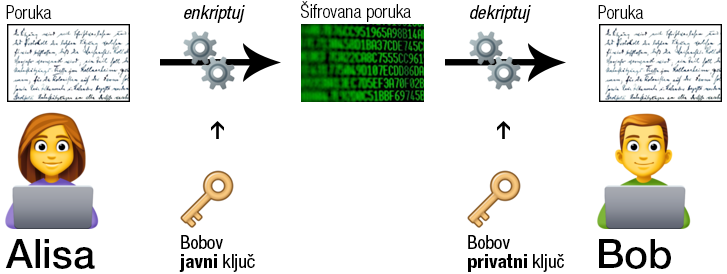
\includegraphics[width=1.0\textwidth]{material/bob_alice_enc}
    \caption{Tajna komunikacija unutar javnog kriptosistema}
    \label{fig:alice_bob_enc}
\end{figure}

\paragraph*{}
Kriptografija javnog ključa također se naziva i \textit{asimetričnom kriptografijom}, ona ne osigurava samo tajnost komunikacije kao u opisanom slučaju, nego se može koristiti i za potvrdu autentičnosti. Za takav scenario dovoljno je da Bob svojim privatnim ključem \textit{potpiše} željenu poruku ili datotetu i Alisa će biti u mogućnosti da provjeri da je ta poruka autentično kreirana od strane Boba, za tu namjenu potrebno je da Alisa posjeduje Bobov javni ključ od ranije ili da ga dobavi iz nekog povjerljivog izvora jer mora biti sigurna da neko lažno ne podmetne svoj ključ kao Bobov, više o ovoj namjeni asimetričnih kriptosistema biti će dato u zasebnom poglavlju u nastavku, no za sada je bitno imati je na umu. Spomenuti proces potpisivanja sastoji se od par kriptografskih operacija, vrlo sličnih kriptovanju poruke, no kako u ovom slučaju nije potrebno prenijeti kompletan sadržaj nego samo omogućiti verifikaciju, proces je moguće učiniti efikasnijim tako što će se poruka prije obrade privatnim ključem prethodno provući kroz neku od hash funkcija, koja će ga znatno smanjiti i ubrzati sam proces.

\subsection{Sigurnosni ciljevi}
Sigurnosni ciljevi kriptografije javnog ključa pored povjerljivosti, kao primarne funkcije, kako je već i pomenuto, uključuju i mogućnosti za provjeru integriteta i autentičnosti poruke, autentifikacija entiteta, te osiguravanje neporecivosti izvršene akcije\cite{buchmann2013introduction}, ovakav jedinstven i širok skup funkcionalnosti kriptografiji javnog ključa daje fundamentalni značaj u modernim digitalnim komunikacijama i internet poslovanju, stoga su osnovne karakteristike svakog od navedenih ciljeva ukratko opisane u nastavku.

\subsubsection*{Povjerljivost i privatnost}
Povjerljivost je osnovni sigurnosni cilj kriptografije i odnosi se na osobinu da tajni podaci neće biti dostupni neautorizovanim osobama. Povjerljivost omogućava privatnost i međusobno su usko povezane. Privatnost označava sposobnost očuvanja vlastitih podataka tajnim za sve one koji nisu eksplicitno autorizovani za njihov pregled i predstavlja osnovno ljudsko pravo garantovano članom 12 Univerzalne deklaracije o ljudskim pravima\cite{assembly1948universal}:

\begin{quote}
\textit{"Niko ne smije biti podvrgnut samovoljnom miješanju u njegovu privatnost, obitelj, dom ili dopisivanje, niti napadima na njegovu čast i ugled. Svako ima pravo na zakonsku zaštitu protiv takvog miješanja ili napada."}
\end{quote}

\paragraph*{}
Mnoštvo je primjera važnosti povjerljivosti i privatnosti u savremenoj eri opšteprisutne digitalizacije i internet poslovanja, nažalost narušavanje ovih temeljnih vrijednosti postalo je gotovo normalna i svakodnevna pojava bilo da se radi o krađi osjetljivih podataka i digitalnih dobara od strane malicioznih agenata ili prisluškivanju od strane korporativnih i vladinih agencija koje vrše masovno špijuniranje na globalnom nivout prikupljanjem privatnih podataka putem raznorodnih programa\cite{wleaks}.

\subsubsection*{Autentifikacija entiteta}
Autentifikacija se odnosi na proces utvrđivanja stvarnog identiteta, navedeni identitet može se odnositi na osobu, kompaniju ili bilo koji drugi koncept koji se od drugog razlikuje po sebi svojstvenim osobinama. Za isti proces može se približno precizno koristiti i termin identifikacija. Poznavanje identiteta u okviru digitalnog okruženje često je neophodno za ispravno funkcionisanje programskog rješenja i pravilnu raspodjelu autorizacija, kao i za relacije povjerenja između različitih kategorija korisnika. Često se za ovu namjenu koriste korisnička imena i lozinke kao najprostiji vid implementacije, no mnogo su pouzdaniji namjenski izrađeni repozitoriji identiteta u vidu specifičnih rješenja ili infrastrukture javnih ključeva (\textit{PKI - public key infrastructure}), koji omogućavaju mnogo sigurniju autentifikaciju, bolje provođenje dobrih sigurnosnih praksi, širi spektar primjene i bolju integraciju. Aplikacija izrađena u okviru ovog rada sadrži namjenski izrađen pokazni repozitorij identiteta i javnih ključeva u vidu Logit API implementacije.

\subsubsection*{Integritet i autentičnost poruke}
Integritet se odnosi na garanciju da podaci nisu mijenjani nakon što ih je izvorni autor sačinio, mnoštvo je bitnih aktivnosti gdje je upravo ovakva garancija od iznimne važnosti. Koncept integriteta dodatno se proširuje kroz pojam autentičnosti poruke, gdje se zahtjeva i mogućnost utvrđivanja njenog izvorišta, te njegova autentifikacija. Ove aktivnosti izvode se putem digitalnog potpisivanja i vjerodostojnih repozitorija koji sadrže provjerene identitete entiteta koji se autoriziraju, najčešće u vidu već opisanih PKI.

\paragraph*{}
Kao primjer možemo uzeti svakodnevno poznate korisničke scenarije, svaki računarski program ili nadogradnja kada se distribuira krajnjim korisnicima može biti naknadno izmjenjen u cilju izvršavanja određenih zlonamjernih aktivnosti koje mogu naštetiti korisniku, da bi se ovo izbjeglo većina savremenih operativnih sistema podržava određeni način provjere integriteta softvera prilikom instalacije na korisničkom računaru i autentičnost identiteta njenog izvorišta, ovakve provjere posebno su bitne u sigurnosno osjetljivim okruženjima i djalatnostima gdje bi pokretanje zlonamjernog koda moglo ugroziti živote ili uzrokovati veliku materijalnu štetu, primjeri takvih sistema su računari u zdravstvu i kontrolni sistemi javnih infrastruktura, poput aerodroma, električne ili vodovodne mreže, no nikako ne treba zanemariti i kućne korisnike koji su itekako izloženi raznim vrstama sigurnosnih prijetnji. Za namjene utvrđivanja integriteta i autentifikacije izvorišta programskih rješenja održavaju se repozitoriji sa identitetima softverskih razvojnih kuća i njihovim ključevima.

\paragraph*{}
Dodatno utvrđivanje integriteta poruke i autentifikacija učesnika se koristi u okviru aplikacije za bilježenje prisustva studenata predložene u okviru ovog rada na način da se potpisano vrijeme i lokacija svih studentskih uređaja potpisuje predavačkim ključevima unutar jedinstvene sesije (npr. nastavnog časa) koju po zaključenju nije moguće naknadno mijenjati bez narušavanja integriteta navedene sesije. Identitet svih učesnika i autentičnost njihovih potpisa provjerava se korištenjem namjenskog repozitorija na Logit API.

\subsubsection*{Neporecivost}
Neporecivost je osobina podataka koja sprječava poduzimača određene aktivnosti da istu porekne nakon njenog okončanja, npr. slanje poruke, novčana transakcija ili prisustvo predavanju. Kod primjera prisustva, radi se o nemogućnosti studenta da nakon što digitalno prijavi svoje prisustvo na predavanju unutar predložene Logit NFC aplikacije naknadno to prisustvo porekne jer postoji jedinstveni digitalno potpisan trag koji to dokazuje, za čvrst dokaz neophodno je osigurati i jaku povezanost korisnika i nosioca identiteta, u ovom slučaju mobilnog uređaja, za ovakve namjene posebno su pogodne višefaktore metode identifikacije koje uključuju i biometrijske osobine.

\section{RSA kriptosistem}
Rivest, Shamir i Adelman\cite{rivest1978method} predložili su kriptosistem koji može osigurati osobine privatnosti i potpisivanja poruka ekvivalentne ili bolje od onih kakve posjeduje papirna pošta. Njihov sistem baziran je na konceptu sistema javnog ključa kakav su ranije predložili Diffie i Hellman\cite{diffie1976new}. Sveukupna procedura sastoji se od procesa enkripcije \textit{E}, procesa dekripcije \textit{D} i poruke \textit{M}, te za takav sistem vrijedi:

\begin{enumerate}
  \item dešifrovanje kriptovane forme poruke \textit{M} daje \textit{M}, \[D(E(M)) = M\]
  \item i \textit{E} i \textit{D} su jednostavne za izračun,
  \item javno obznanjujući \textit{E} korisnik ne otkriva jednostavan način za izračun \textit{D}. Praktično ovo znači da samo on može dekriptovati poruke kriptovane pomoću \textit{E}
  \item ukoliko je poruka \textit{M} prvo dešifrovana a onda šifrovana, rezultat je \textit{M}, \[E(D(M)) = M\]
\end{enumerate}

\paragraph*{}
Enkripcijska (ili dekripcijska) procedura se sastoji od \textit{opšte metode} i \textit{enkripcijskog ključa}. Opšta metoda, pod kontrolom ključa, šifruje poruku \textit{M} i rezultira šifrovanom porukom \textit{C (en. ciphertext)}. Svako može koristiti istu opštu metodu, sigurnost date procedure počiva na sigurnosti ključa. Otkrivanje enkripcijskog algoritma tada znači i otkrivanje (\textit{javnog}) ključa.

\paragraph*{}
Kada korisnik otkrije \textit{E}, on otkriva vrlo neefikasan način izračuna \textit{D(C)} testiranjem svih mogućih poruka \textit{M} sve dok se ne nađe ona koja zadovoljava \(E(M) = C\). Ukoliko je osobina (3) zadovoljena broj takvih poruka nije praktičan za izračun.

\paragraph*{}
Funkcija \textit{E} ukoliko zadovoljava osobine (1)-(3) predstavlja tzv. \textit{"jednosmjernu funkciju sa stupicom"}, a ukoliko zadovoljava i (4) onda je \textit{"jednosmjerna permutacija sa stupicom"}. Diffie i Hellman\cite{diffie1976new} uveli su koncepte jednosmjernih funkcija sa stupicom ali nisu dali implementaciju. Ove funkcije nazivaju se jednosmjernim jer ih je jednostavno izračunati u jednom smijeru ali bi trebalo biti vrlo teško u suprotnom, dok su "sa stupicom" jer su njihovi inverzi jednostavni za izračun ukoliko je poznata određena informacija, u slučaju šifrovanja je to privatni ključ. Ovakva funkcija koja također zadovoljava i (4) mora biti permutacija: svaka poruka je ciphertekst neke druge poruke i svaki ciphertekst je dozvoljena poruka. Zadovoljenje osobine (4) neophodno je za implementaciju potpisivanja.

\subsection{Ključevi i komunikacija} \label{subs:keygen}
Da bi kreirali vlastite privatne i javne ključeve učesnici moraju svaki za sebe i nasumično odabrati dva velika prosta broja \textit{p} i \textit{q} takva da nije vjerovatno da računar može izvršiti cjelobrojnu faktorizaciju \(n = p * q\), danas se minimalno preporučuju brojevi slične veličine koji daju proizvod reda 2048 bita kao sigurni do 2030. godine\cite{kaliski2003twirl}. Proizvod \textit{n} postaje dijelom javnog ključa, dok se pojedinačni faktori moraju čuvati u tajnosti zbog njihovog korištenja u derivaciji privatnog ključa.

\paragraph*{}
Korisnici također moraju izabrati i cjelobrojnu vrijednost \textit{e} takvu da, \[1 < e < \phi(n) = (p - 1)(q - 1) \wedge \gcd(e, (p - 1)(q - 1) = 1.\] Obratite pažnju da je e uvijek neparno jer je \((p - 1)(q - 1)\) parno. Dalje korisnik računa cjelobrojnu vrijednost \textit{d}, \[1 < d < (p - 1)(q - 1) \wedge de \equiv 1\bmod(p - 1)(q - 1).\] Korisnikov javni ključ sada je par \textit{(n, e)}, dok je njegov privatni ključ \textit{d}. Broj n naziva se \textit{RSA modulus}, \textit{e} je \textit{enkripcijski eksponent}, a \textit{d - dekripcijski eksponent}\cite{buchmann2013introduction}.

\paragraph*{}
Ponovno se može poslužiti primjerom Boba i Alise opisanim ranije, sada se može reči da kada je Bob korištenjem opisane procedure generisao neophodne vrijednosti ključeva i poslao Alisi svoj javni ključ, tj. vrijednosti \textit{(n, e)}, koje će ona iskoristiti za šifrovanje proizvoljne poruke \textit{m}, što tada možemo izraziti kao \[c = m^e\bmod n.\] Kada Bob primi Alisinu šifrovanu poruku \textit{c} iskoristiti će tajnu vrijednost \textit{d} i dešifrovati poruku \[m = c^d\bmod n.\]

\subsection{Digitalni potpis}
Digitalni potpis osigurava mehanizam provjere integriteta i u kombinaciji sa adekvantnom infrastrukturom - autentičnost izvorišta poruke. Ukoliko Bob želi potpisati određeni dokument, on korištenjem svog privatnog ključa izračunava jedinstveni niz bita, koji Alisi garantuje da će korištenjem Bobovog prethodno dobavljenog javnog ključa moći verifikovati da navedeni dokument nije izmjenjen u putu do nje, kao i da je Bob originalni potpisnik dokumenta, navedena interakcija prikazana je na slici \ref{fig:alice_bob_sig}, dodatno Bob u budućnosti ne može poreči da je potpisao navedeni dokument, što osigurava još jednu vrlo bitnu funkcionalnost cjelokupnog sigurnosnog sistema. Ovakav sistem predstavlja temelj na kojem je izgrađen siguran internet i digitalna ekonomija te je duboko utkan u osnovne protokole poput TLS, SSH, PGP etc.

\begin{figure}[H]
    \centering
    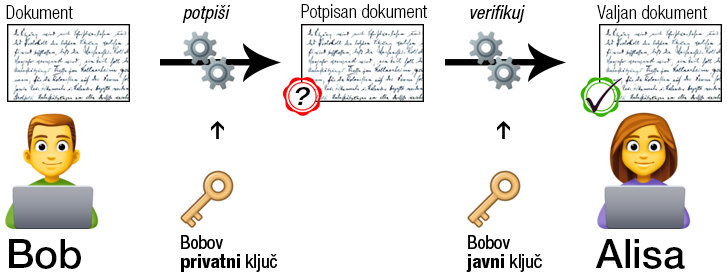
\includegraphics[width=1.0\textwidth]{material/bob_alice_sig}
    \caption{Verifikacija integriteta i autentičnosti uz garancija neporecivosti u okviru javnog kriptosistema}
    \label{fig:alice_bob_sig}
\end{figure}

\paragraph*{}
RSA šema najčešće je korišten algoritam digitalnog potpisivanja. Generacija ključeva funkcionira na istom principu kao i u primjeru šifrovanja poruke opisanom u poglavlj \ref{subs:keygen}. Svaki digitalni potpis zavisan je od poruke kao i od potpisnika, u protivnom bilo bi moguće da isti potpisnik koristi jedan potpis za više dokumenata, što ovdje nije slučaj. Da bi se uspješno implementiralo digitalno potpisivanje, kriptosistem mora zadovoljavati osobine spomenute jednosmjerne permutacije sa stupicom, budući da će dekripcijski algoritam biti primjenjivan na izvorni - nešifrovan dokument.

\paragraph*{}
Opisani primjer razmjene potpisanog dokumenta ili poruke \textit{M} između Alise i Boba može se unutar RSA kriptosistema preciznije prikazati kao: \[S = D_{B}(M),\] gdje je \textit{S} digitalno potpisana poruka a \(D_{B}\) Bobova funkcija za dešifrovanje korištenjem privatnog ključa. Kako je već napomenuto primjena funkcije za dešifrovanje na nešifrovanu poruku ima smisla u slučaju da kriptosistem zadovoljava potrebne uvjete. Ukoliko je dodatno potrebno osigurati i tajnost potpisane poruke Bob je može naknadno šifrirati Alisivnim javnim ključem, u tom slučaju Alisa po prijemu prvo vrši dešifrovanje svojim privatnim ključem da bi dobila Bobovu izvornu potpisanu poruku \textit{S}, korištenjem Bobovog javnog ključa Alisa sada "šifruje" potpisanu poruku \[M = E_{B}(S)\] time dolazeći u posjed uređenog para \textit{(M, S)} sa osobinama sličnim onima koje ima originalni fizički potpisan dokument.

\paragraph*{}
Sama praktična implementacija potpisivanja razlikuje se međutim od opisane procedure u tome da se u praksi ne vrši potpisivanje cjelokupne izvorn poruke, nego se nad njom prvobitno korištenjem hash funkcije otporne na kolizije izračunava jedinstvena hash vrijednost, pa Bob tako umjesto poruke potpisuje dobijenu hash vrijednost svojim privatnim ključem, dok na drugom kraju Alisa ponavlja proces izračunavanja hash vrijednosti koristeći Bobovu izvornu poruku, njegov javni ključ i istu hash funkciju, te dobijeni hash poredi sa Bobovim hashom, u slučaju poklapanja vrijednosti Alisa može biti sigurna u valjanost digitalnog potpisa. Jedina funkcionalna razlika ovakvog pristupa je da se koncept poruke ili dokumenta, odvaja od samog digitalnog potpisa, što olakšava rad i osigurava dodatne sigurnosne i upotrebne prednosti.

\paragraph*{}
Praktična implementacija može se formalno opisati kao primjena hash funkcije \textit{h} tako da potpis \textit{s} niza karaktera poruke \(m \in \lbrace 0,1\rbrace ^n\) glasi \[s = h(m)^d\bmod n.\] \textit{d} je u prikazanom slučaju Bobov \textit{dekripcijski eksponent}. Da bi Alisa verifikovala zaprimljeni potpis \textit{s} koristi Bobov javni ključ \textit{(n, e)} i izračunavanjem hash vrijednost \textit{h(m)} poruke \textit{m} i vrši provjeru \[h(m) = s^e\bmod n.\] Potpis je valjan ako i samo ako važi data jednakost. Za potrebe Logit sistema korištena je SHA-256 hash funkcija u kombinaciji sa RSA potpisom.

\pagebreak[4]

\section{PKI - infrastruktura javnog ključa}
Iako kriptografija javnog ključa ne zahtjeva razmjenu tajnih ključeva da bi se ostvarila povjerljiva komunikacij, vrlo je bitan aspek upravljanja ključevima, kako javnim tako i privatnim. Namjena infrastrukture javnog ključa \textit{en. PKI - private key infrastructure} je upravo to, efikasno i sigurno upravljanje javnim i privatnim ključevima tokom njihovog životnog ciklusa.

\subsection{Životni ciklus ključeva}
Životni ciklus počinje od samog generisanja, koje je opisano u poglavlju \ref{subs:keygen}, nakon čega slijedi upotrebni vijek tokom kojeg se privatni ključevi koriste za potpisivanje ili dešifrovanje primljenih poruka. Korisnici također imaju pristup javnim ključevima drugih korisnika, te ključeve koriste za šifrovanje ili verifikaciju potpisanih dokumenata. U završnoj fazi ključevi izlaze iz upotrebe bilo kroz proces zastarjevanja ili neki drugi događaj. Svaki od navedenih faza u životnom ciklusu para ključeva mora imati određene procedure da bi se osiguralo provođenje dobrih praksi u njihovom upravljanju.

\subsubsection{Generisanje i pohrana}
Prvi korak je osiguravanje pouzdanog okruženja za generisanje sigurnog para ključeva, najbolje je da tu aktivnost izvode sami korisnici, jer u tom slučaju privatni ključ ne bi trebao biti dostupan nijednoj trećoj strani, no to često nije slučaj, budući da korisničko okruženje može biti kompromitovano ili na neki drugi način neadekvatno za tu namjenu, stoga se mora pribjeći generisanju ključeva u okruženju neke povjerljive treće strane za koju se može biti sigurno da ključeve neće zloupotrijebiti. Pored navedenog i samo skladištenje ključeva, pogotovo privatnih, pruža mnoge sigurnosne izazove. Uzimajući u obzir nabrojano jasno je da navedenim problemima treba pristupiti planski i krajnje ozbiljno jer u protivnom sigurnost kompletnog sistema može biti kompromitovana od samog početka. Logit aplikacija privatne ključeve pohranjuje isključivo unutar Android repozitorija ključeva na korisničkom uređaju, za koji postoje garancije da nije moguće ostvariti pristup korištenjem bilo koje druge aplikacije.

\subsubsection{Upotrebni vijek}
Tokom upotrebne faze životnog vijeka osnovna funkcionalnost je obezbjediti siguran pristup korisničkim javnim ključevima. Pored toga da bi se mogle pružiti adekvatne garancije autentifikacije i potvrde autentičnosti neophodno je utvrditi i provesti jasne procedure koje će osigurati jasnu povezanost entiteta/osoba sa ključevima, u protivnom može doći do krađe identiteta i lažnog predstavljanja. Logit API vršit funkciju repozitorija javnih ključeva za korisnike sistema i povezuje korisnike sa njihovim ključevima, osigurana je osnovna provjera identiteta putem korisničke prijave na fakultetski ZAMGER sistem.

\subsubsection{Kraj životnog ciklusa}
Dodatno potrebno je utvrditi jasne procedure za kraj životnog vijeka i pohranu starih ključeva, kod Logit API repozitorija ne postoji vremenski ograničen vijek trajanja para ključeva, no pri svakoj novoj instalaciji aplikacije ili zamjeni uređaja, stari par ključeva se arhivira a novogenerisani ključevi se koriste kao sigurnosno relevantni. Pored navedenih funkcionalnosti Logit API se koristi i kao repozitorij potpisanih dokumenata, u ovom slučaju, prisutava predavanjima, no to izlazi iz okvira domena PKI i može se smatrati dodatno funkcionalnošću.

\subsection{Hijerarhija povjerenja}
Za praktičnu upotrebu kriptografije javnog ključa neophodno je da korisnici vjeruju u autentičnost dostupnih javnih ključeva. Stoga su pored prostog direktnog modela povjerenja sa dva učesnika koji razmjenjuju sopstvene javne ključeve uspostavljene raznovrsne hijerarhije povjerljivih učesnika koje omogućavaju formiranje složene mreže koja i sama kao svoju osnovu koristi digitalni potpis i dostupne kriptografske metode.

\begin{figure}[H]
    \centering
    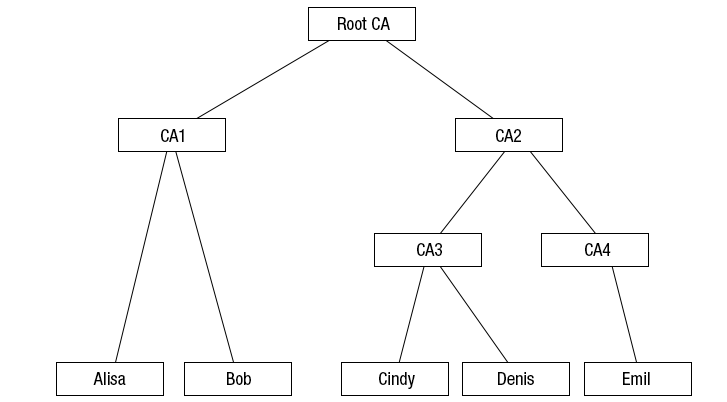
\includegraphics[width=1.0\textwidth]{material/pki}
    \caption{Primjer hijerarhijske infrastrukture javnog ključa}
    \label{fig:pki}
\end{figure}

\paragraph*{}
Primjer jedne složene hijerarhije povjerenja prikazan je na slici \ref{fig:pki}, u ovakvom modelu javne ključeve svih nižih učesnika potvrđuje CA \textit{(en. certification authority)}, koji ujedno na adekvatan način vrši i verifikaciju autentičnosti. Većina ovakvih hijerarhijskih PKI arhitektura uređena je u skladu sa standardom X.509. U ovakvom okruženju može da učestvuje više nivoa posrednih CA \textit{(en. intermediate CA)} i obično je uređeno u strukturu drveta sa listovima, gdje se u korjenu nalazi CA \textit{(en. root CA)} kojeg svi posredni CA uzimaju kao pouzdanog i koji sam potpisuje svoj certifikat. Na dnu strukture drveta nalaze se krajnji korisnici kriptosistema. Da bi se ostvarila relacija povjerenja između dva korisnika, nije neophodno da oni dijele isti posredni CA, dovoljan uslov je da se može napraviti veza prema jednom CA u kojeg oba korisnika imaju povjerenje da bi pomenuta relacija bila zadovoljena.

\paragraph*{}
Primjer jedne relacije povjerenja iz priložene hijerarhije može se formirati između korisnika Alisa i Emil, gdje se da jasno utvrditi \textit{certifikacijska putanja} koja za oba korisnika seže do korjenskog Root CA, ilustrativno za Alisu i Emila važi: \[Alisa \to CA1 \to Root CA\] \[Emil \to CA4 \to CA2 \to Root CA\] dubina certifikacijske putanje također može da igra ulogu u zavisnosti od različitih zahtjeva, u nekim slučajevima duže putanje, poput Emilove se mogu smatrati nepouzdanim za određene namjene, u svakom slučaju poželjno je korištenje što bližih međusovnih putanja.

\paragraph*{}
Logit API posjeduje svoj set ključeva kojim potpisuje sve zaprimljene korisničke sesije prisustva. Da bi se upotpunio model povjerenja neophodno je da se LAPI ceritikat potvrdi od strane institucije koja implementira navedeni sistem, u ovom slučaju Elektrotehničkog fakulteta, koja je dalja poveznica na vanjski korjenski CA i omogućava izgradnju šireg sistema povjerenja gdje više institucija koje koriste isti sistem može ostvariti posredne relacije povjerenja. Važno je istaknuti također da korisnici registracijom bivaju uključeni u LAPI repozitorij, što se može smatrati ekvivalentom certifikata, dodatno korisnici međusobno potvrđuju prisustvo a samim tim ostvaruju vezu međusobnog povjerenja, jer aktivnost prikupljanja potpisa inherentno utvrđuje međusobnu identifikaciju korisnika. Prikaz takvog modela dat je na slici \ref{fig:logit_pki}.

\begin{figure}[H]
    \centering
    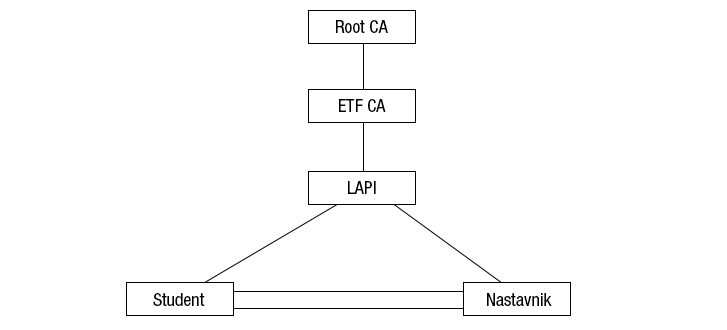
\includegraphics[width=1.0\textwidth]{material/logit_pki}
    \caption{Prikaz Logit PKI hijerarhije}
    \label{fig:logit_pki}
\end{figure}

\subsection{Certifikati}
Bitan aspekt PKI je obezbjeđivanje potvrde autentičnosti za javne ključeve, jedan od načina da se to ostvari su svakako certifikati, tj. strukture koje povezuju javne ključeve sa entitetima ili osobama, najčešće su pohranjeni na PKI koji se brinu da osiguravaju što jaču garanciju relacije između entiteta i javnog ključa. U cilju iskoristivosti neophodno je da certifikati obezbjede određeni nivo tehničkih i domenski relevantnih podataka, u većini slučajeva to su:

\begin{itemize}
    \item ime ili naziv entiteta za čiji javni ključ je vezan
    \item javni ključ entiteta
    \item korišteni kriptografski algoritam
    \item serijski broj
    \item period važenja
    \item naziv izdavača certifikata, koji je ujedno i potpisnik
    \item namjena i ograničenja korištenja javnog ključa
\end{itemize}

\paragraph*{}
Sam sadržaj certifikata u većini slučajeva je standardiziran, danas najčešće standardom X.509, gdje se i izdati certifikat naziva prema standardu X.509 certifikat, primjer jednog takvog certifikata dat je na slici \ref{img:etf_cert_gen}, navedene su osnovne informacije o certifikatu i opšte informacije pobrojane iznad, dodatno na slici \ref{img:etf_cert_tree} prikazana je certifikacijska putanja datog certifikata. Pored navedenih informacija certifikat obično sadrži mnoštvo i drugih informacija, budući da standard dopušta proširivanje da bi obuhvatio širok domen primjene. Bitno je još napomenuti da zbog vrlo široke primjene u različitim programskim rješenjima postoji mnoštvo različitih formata zapisivanja i razmjene samih certifikata, te je često neophodno konvertovati certifikate u jedan od odgovarajućih formata.

\paragraph*{}
X.509 certifikati koriste ASN.1 \textit{(en. abstract syntax notation version 1)} kao jezik za izvornu specifikaciju osobina certifikata, pomoću navedenog jezika moguće je izraziti mnoštvo kompleksnih struktura za opis osobina certifikata, jedan od mnoštva načina da se navedena specifikacija zapiše je DER \textit{(en. distinguished encoding rules)}, koja je dalje bazirana na BER pravilima za zapisivanje \textit{(en. basic encoding rules)}, navedene strukture predstavljaju svojevrsnu hijerarhiju deskriptivnih jezika i meta-jezika sličnu relaciji SGML, HTML.

\begin{figure}[H]
    \centering
    \begin{subfigure}{.5\textwidth}
        \centering
        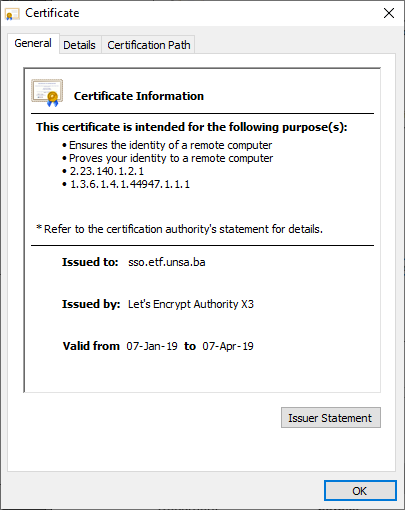
\includegraphics[width=1\textwidth]{material/etf_cert_gen}
        \caption{opšte karakteristike}
        \label{img:etf_cert_gen}
    \end{subfigure}%
    \begin{subfigure}{.5\textwidth}
        \centering
        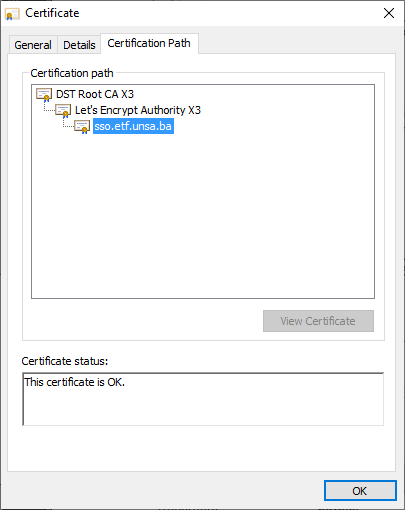
\includegraphics[width=1\textwidth]{material/etf_cert_tree}
        \caption{lanac povjerenja}
        \label{img:etf_cert_tree}
    \end{subfigure}
    \caption{Osobine certifikata}%
    \label{img:etf_cert}
\end{figure}

\paragraph*{}
Logit aplikacija interno koristi namjenski i nestandardni format certifikata, no sve LAPI i korisničke certifikate moguće je pretvoriti u bilo koji od standardnih formata i tako ostvariti interakciju sa ostalim sistemima ukoliko se za to ukaže potreba. Dovoljno je na Logit API strani implementirati novu URI lokaciju koja bi vraćala certifikate u standardizovanom formatu.
%	\chapter{Prijedlog rješenja}
U skladu sa datim zahtjevima predložena je izrada aplikacijske platforme pod nazivom Logit (
\gls{LAPP}), opisane u nastavku, sa detaljnim tehničkim detaljima u narednim poglavljima. Uzimajući u obzir data ograničenja, te funkcionalne i nefunkcionalne zahtjeve određeno je da se korisnička aplikacija izradi na Android platformi sa podrškom za Android API nivo počevši od nivoa 19 (4.4 KitKat), to je najniži nivo koji omogućava korištenja naprednih NFC i kriptografskih funkcionalnosti te osigurava dobru pokrivenost potencijalne korisničke baze sa ukupnom adopcijom od preko 90\% za navedenu ili višu verziju\cite{droidstats}. Za uspješan rad aplikacije neophodno je da korisnički uređaj podržava i NFC funkcionalnosti, prema prognozama analitičke kuće IHS Technology, do 2020. godine svaki treći uređaj imati će podršku za NFC.\cite{nfcforecast}

\section{Logički model rješenja}
Priloženi dijagrami interakcije osnovnih funkcionalnosti Logit platforme i pripadajući opis imaju za cilj stvoriti opštu sliku sistema, te tako olakšati praćenje tehničkog modela rješenja datog u nastavku. Tehnički model opisuje dosta detaljniju sliku funkcioniranja sistema i može služiti kao svojevrstan uvod u kod platforme.

\subsection*{Registracija korisnika}
\begin{figure}[H]
    \centering
    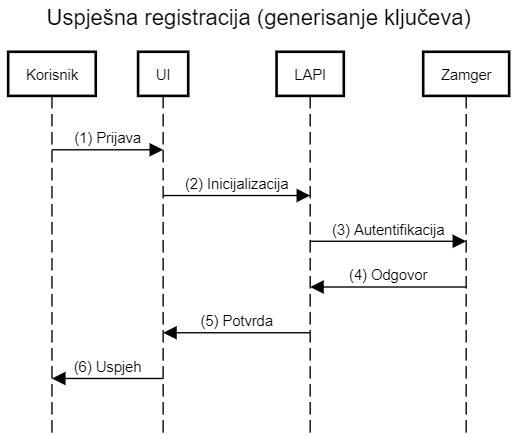
\includegraphics[width=0.7\textwidth]{material/dia/01_registracija}
    \caption{Dijagram interakcije - uspješna registracija i generisanje ključeva}
\end{figure}
\paragraph*{}
Nakon uspješne instalacije aplikacije na korisnički Android uređaj (DEVICE) potrebno je obaviti proces registracije koji se izvršava u dva bitna koraka. Prvi korak sastoji se od unosa već postojećih autentifikacijskih podataka za ZAMGER sistem Elektrotehničkog fakulteta, korisnik se korištenjem datih podataka posredstvom LAPI servisa autentificira na ZAMGER sistemu, bitno je napomenuti da Logit platforma ne sprema korisničku lozinku ZAMGER sistema, navedeni podaci se koriste isključivo za povezivanje postojećeg identiteta i novogenerisanog para korisničkih RSA ključeva (KEYS), što je ujedno i drugi korak u procesu registracije na Logit platformu.

\paragraph*{}
U slučaju uspješnje autentifikacije, korisnika se obavještava o završenoj registraciji te se preusmjerava na glavni ekran za bilježenje prisustva. Generisani javni ključ (CERT) i identifikacioni podaci korisnika spremaju se u LAPI direktorij korisničkih certifikata.

\subsection*{Bilježenje prisustva studenta}
Bilježenje prisustva studenata od strane predmetnog nastavnika izvodi se u Master (M) modu funkcionisanja aplikacije, aplikacija se pri samom pokretanju i nakon uspješno obavljene registracija automatski stavlja u takav mod operacije i u njemu ostaje sve dok je upaljen ekran korisničkog uređaja (DEVICE) i Logit aplikacija (UI) se izvršava u prednjem planu \textit{(en. foreground)}, navedene zahtjeve diktira sama Android platforma.

\begin{figure}[H]
    \centering
    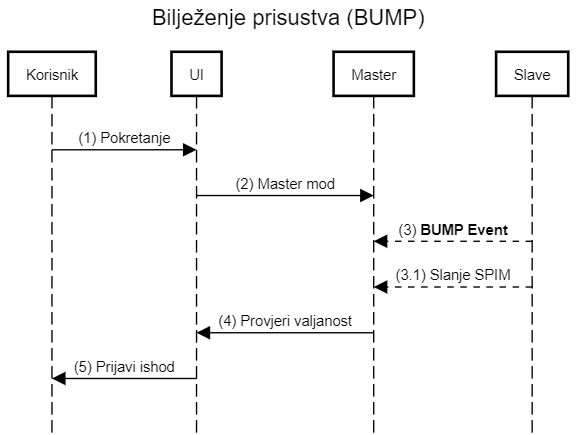
\includegraphics[width=0.7\textwidth]{material/dia/02_bump}
    \caption{Dijagram interakcije - bilježenje prisustva studenata (Master BUMP)}
\end{figure}
\paragraph*{}
Ukoliko su ispunjeni prethodno pobrojani zahtjevi, dovoljno je da student sa podešenom Logit aplikacijom na svom uređaju prinese slave (S) uređaj master (M) uređaju i da njegovo prisustvo bude zabilježeno i prikazano na ekranu M uređaja. Samu interakciju (BUMP) inicira studentski S uređaj. Prilikom ovog BUMP događaja dolazi do razmjene kriptografski potpisanih podataka o vremenu i lokaciji (SPIM) sa S na M, gdje M vrši validaciju primljenih podataka poredeći studentsko vrijeme i lokaciju sa vremenom i lokacijom na M uređaju, gdje se prisustvo odbija ukoliko se ustanovi pokušaj lažiranja podataka.

\subsection*{Prijava prisustva}
\begin{figure}[H]
    \centering
    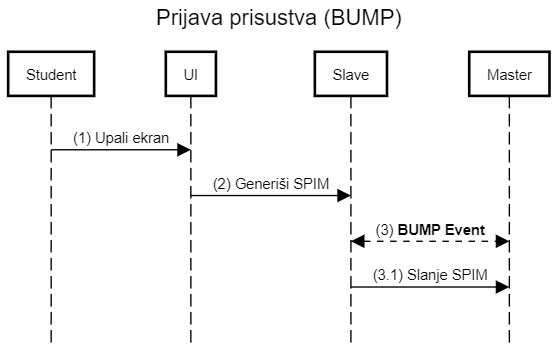
\includegraphics[width=0.7\textwidth]{material/dia/03_prijava}
    \caption{Dijagram interakcije - prijava prisustva studenta (Slave BUMP)}
\end{figure}

\paragraph*{}
Studentski S uređaj i M uređaj nastavnog osoblja podešavaju se na isti način opisan iznad, jedina praktična razlika javlja se prilikom korištenja, gdje je za S uređaj čije se prisustvo bilježi dovoljno upaliti ekran uređaja da bi se mogla ostvariti BUMP interakcija prislanjanjem S na M. Ovo je moguće jer se NFC HCE emulator Logit aplikacije izvršava u pozadini Android sistema.

\subsection*{Pohranjivanje potpisa sesije na LAPI}
Svako bilježenje prisustva unutar Logit Android UI odvija se unutar sesije (SESS) koja se automatski započinje prilikom prvog uspješno zabilježenog prisustva i traje sve dok korisnik ne izvrši pohranu navedene sesije na LAPI servis. Klikom na SYNC dugme prikupljeni podaci šalju se LAPI servisu, provjeravaju se jedinstveni potpisi studenata te potpis ukupne sesije od strane M uređaja, ukoliko se ne pronađu nepravilnosti navedeni podaci se pohranjuju u LAPI repozitorij potpisa, takvi podaci kriptografski su osigurani od naknadne izmjene.

\begin{figure}[H]
    \centering
    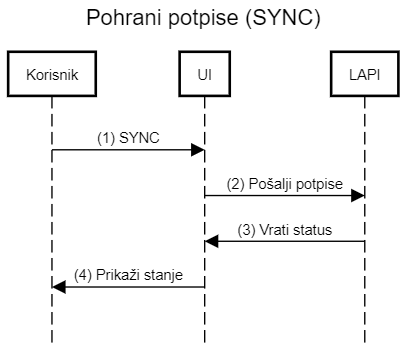
\includegraphics[width=0.6\textwidth]{material/dia/04_sync}
    \caption{Dijagram interakcije - pohranjivanje potpisa na LAPI (SYNC)}
\end{figure}
\paragraph*{}
Potpisi pohranjeni u LAPI repozitoriju mogu dalje biti korišteni u integrisanim aplikacijskim rješenjima koja zahtijevaju ovakvu vrstu podataka pomoću ponuđenog LAPI REST interfejsa, te se mogu smatrati relevantnim i sigurnim dokazom prisustva.

\section{Tehnički model rješenja}
Uvodi se dodatno pojam lokacijskog dokaza\cite{locproof} koji u širem smislu u kontekstu podređenog korisnika (en. slave), obuhvata kriptografski potpisan korisnički identitet, korisnički uređaj, vrijeme i GPS lokacijske podatke korisničkog uređaja. Za svrhu osiguranja jedinstvenosti identiteta i vjerodostojnosti potvrde lokacijskih dokaza odabrano je korištenje RSA asimetrične enkripcije, gdje se pri uspješnoj autentifikaciji generiše jedinstveni set ključeva za korisnički uređaj, privatnom dijelu ključa nije moguće pristupiti izvan aplikacije (SEC1), niti je moguće eksportovati ključ (SEC2), a u određenom vremenskom period može postojati samo jedan valjan set ključeva za jednog korisnika jer se raniji ključevi ne uzimaju u obzir ukoliko postoji noviji set (SEC3), sprječavajući tako replikaciju identiteta na više uređaja.

\paragraph*{}
Pored Android komponente aplikacije (UI) izrađena je i serverska aplikacija u programskom jeziku Python (LAPI), čija je namjena posredovanje u komunikaciji sa autentifikacijskim agentom (ZAMGER), te pohranjivanja i održavanje javnih korisničkih kriptografskih ključeva (CERT) i njihovo povezivanje sa autentifikacijskim podacima korisnika, pored toga služi i kao repozitorij za potpisana prisustva (ATTN). Na ovu komponentu se može gledati kao na integrisani namjenski repozitorij korisničkih certifikata i domenski repozitorij neporecivih i neizmjenjivih lokacijskih dokaza (SPIM).

\paragraph*{}
Budući da na Elektrotehničkom fakultetu u Sarajevu postoji SSO (en. Single-Sign On) politika autentifikacije, u serverskoj komponenti (LAPI) je implementiran autentifikacijski posrednik koji prilikom prvog pokretanja aplikacije prijavljuje korisnika koristeći postojeće pristupne podatke, tom prilikom u slučaju uspješne prijave generiše se i jedinstveni set RSA ključeva dužine 2048 bita (KEYS), koji se pohranjuju na korisničkom uređaju (DEVICE), a javni dio, tj. certifikat (CERT) se pohranjuje i u repozitorij ključeva (LAPI) sa poveznicom na korisnički identitet, kasnije se ti certifikati koriste za provjeru valjanosti potpisa lokacijskih dokaza (SPIM).

\paragraph*{}
Da bi se osigurala jednostavnost korištenja aplikacije odabrana je implementacija HCE emulacijskog načina rada NFC komunikatora koji omogućava korisniku da izvrši komunikaciju sa drugim uređajem bez potrebe da pokreće aplikacijski prozor na svom uređaju, dovoljno je da upali ekran svoj uređaja i prinese ga master (M) uređaju koji prikuplja potpise, u ovom slučaju drugoj instanci Logit aplikacije na kojoj je pokrenuta aktivnost za prikupljanje potpisa (LAPP).

\paragraph*{}
Približavanjem mobilnih uređaja (BUMP) otvara se jednosmjerni komunikacijski kanal u smijeru od slave (S) prema master (M) uređaju korištenjem ISO/IEC 14443 Tip A komunikacijskog protokola pri čemu se emulira NFC Forum Tag tipa 4 i putem NDEF Aplikacije prenosi jedna NDEF poruka (NDEFMSG) koja sadrži vremensko-lokacijski dokaz potpisan od strane korisnika, nadalje u tekstu označen kao SPIM (en. spime)\cite{bruces}.

\paragraph*{}
Po primitku poruke nadređeni uređaj (en. master) koji osluškuje da mu se pridruže podređeni uređaji (en. slave) i ima pokrenutu Logit aplikaciju, tu poruku sprema u lokalni repozitorij potpisa ukoliko ona zadovolja uslove da očitana slave GPS lokacija nije udaljena više od 50 metara od očitane master GPS lokacije (VK1 - validacijski kriterij \#1), te da podešena razlika satova master i slave uređaja nije veća od 300 sekundi (VK2), bez da nad SPIM objektom vrši ikakve izmjene, ukoliko SPIM objekat ne zadovoljava date validacijske kriterije odbija se i ispisuje se odgovarajuća poruka na master ekranu. Moguće je naknadno klikom na validacijsko dugme (ACTVAL) u korisničkom interfejsu izvršiti provjeru svih prikupljenih potpisa tokom jedne sesije (SESS), tom prilikom se, ukoliko postoji mrežna veza; svi potpisi pošalju Logit serveru (LAPI) na provjeru i vraća se stanje valjanosti potpisa za sve proslijeđene SPIM objekte.

\paragraph*{}
Ukoliko master (M) želi da pohrani SPIM objekte iz jedne sesije (SESS) na Logit server (LAPI), klikom na sinhronizacijsko dugme u interfejsu (ACTSYNC), on vrši dodatno potpisivanje svakog SPIM objekta svojom komponentom privatnog ključa (MPRK), tako što potpiše hash (SHA256) vrijednost SPIM objekta (AID) sa dodatim svojim jedinstvenim master korisničkim imenom (MUSER) i jedinstvenim identifikatorom sesije (SID) i dodatno generiše SHA256 vrijednosti tih potvrda (CID), nakon čega objedinjuje sve CID vrijednosti i dodatno ih potpisuje svojim MPRK, sve te vrijednosti šalje Logit server (LAPI) na pohranjivanje, ovakvom procedurom se obezbjeđuje neporecivost i neizmjenjivost SPIM i SESS objekata, jer onemogućava izmjene pojedinačnih SPIM objekata, te brisanje ili dodavanje objekata u finaliziranoj sesiju (SESS) od strane malicioznih aktera bez da naruši integritet SHA256 vrijednosti.

\paragraph*{}
Uzmimajući u obzir bitnost rješenja i visoku vjerovatnoću svakodnevne primjene kod ciljane korisničke grupe, te izazove koje takav slučaj korištenja predstvalja omogućena je i direktna e-mail komunikacija za prijavu grešaka ili slanje prijedloga sa glavnog korisničkog interfejsa (ACTBUG). Kako se radi o slojevitom i kompleksnom softverskom rješenju za više detalja referirati se na izvorni kod priložen u dodatku.

\begin{figure}[H]
    \centering
    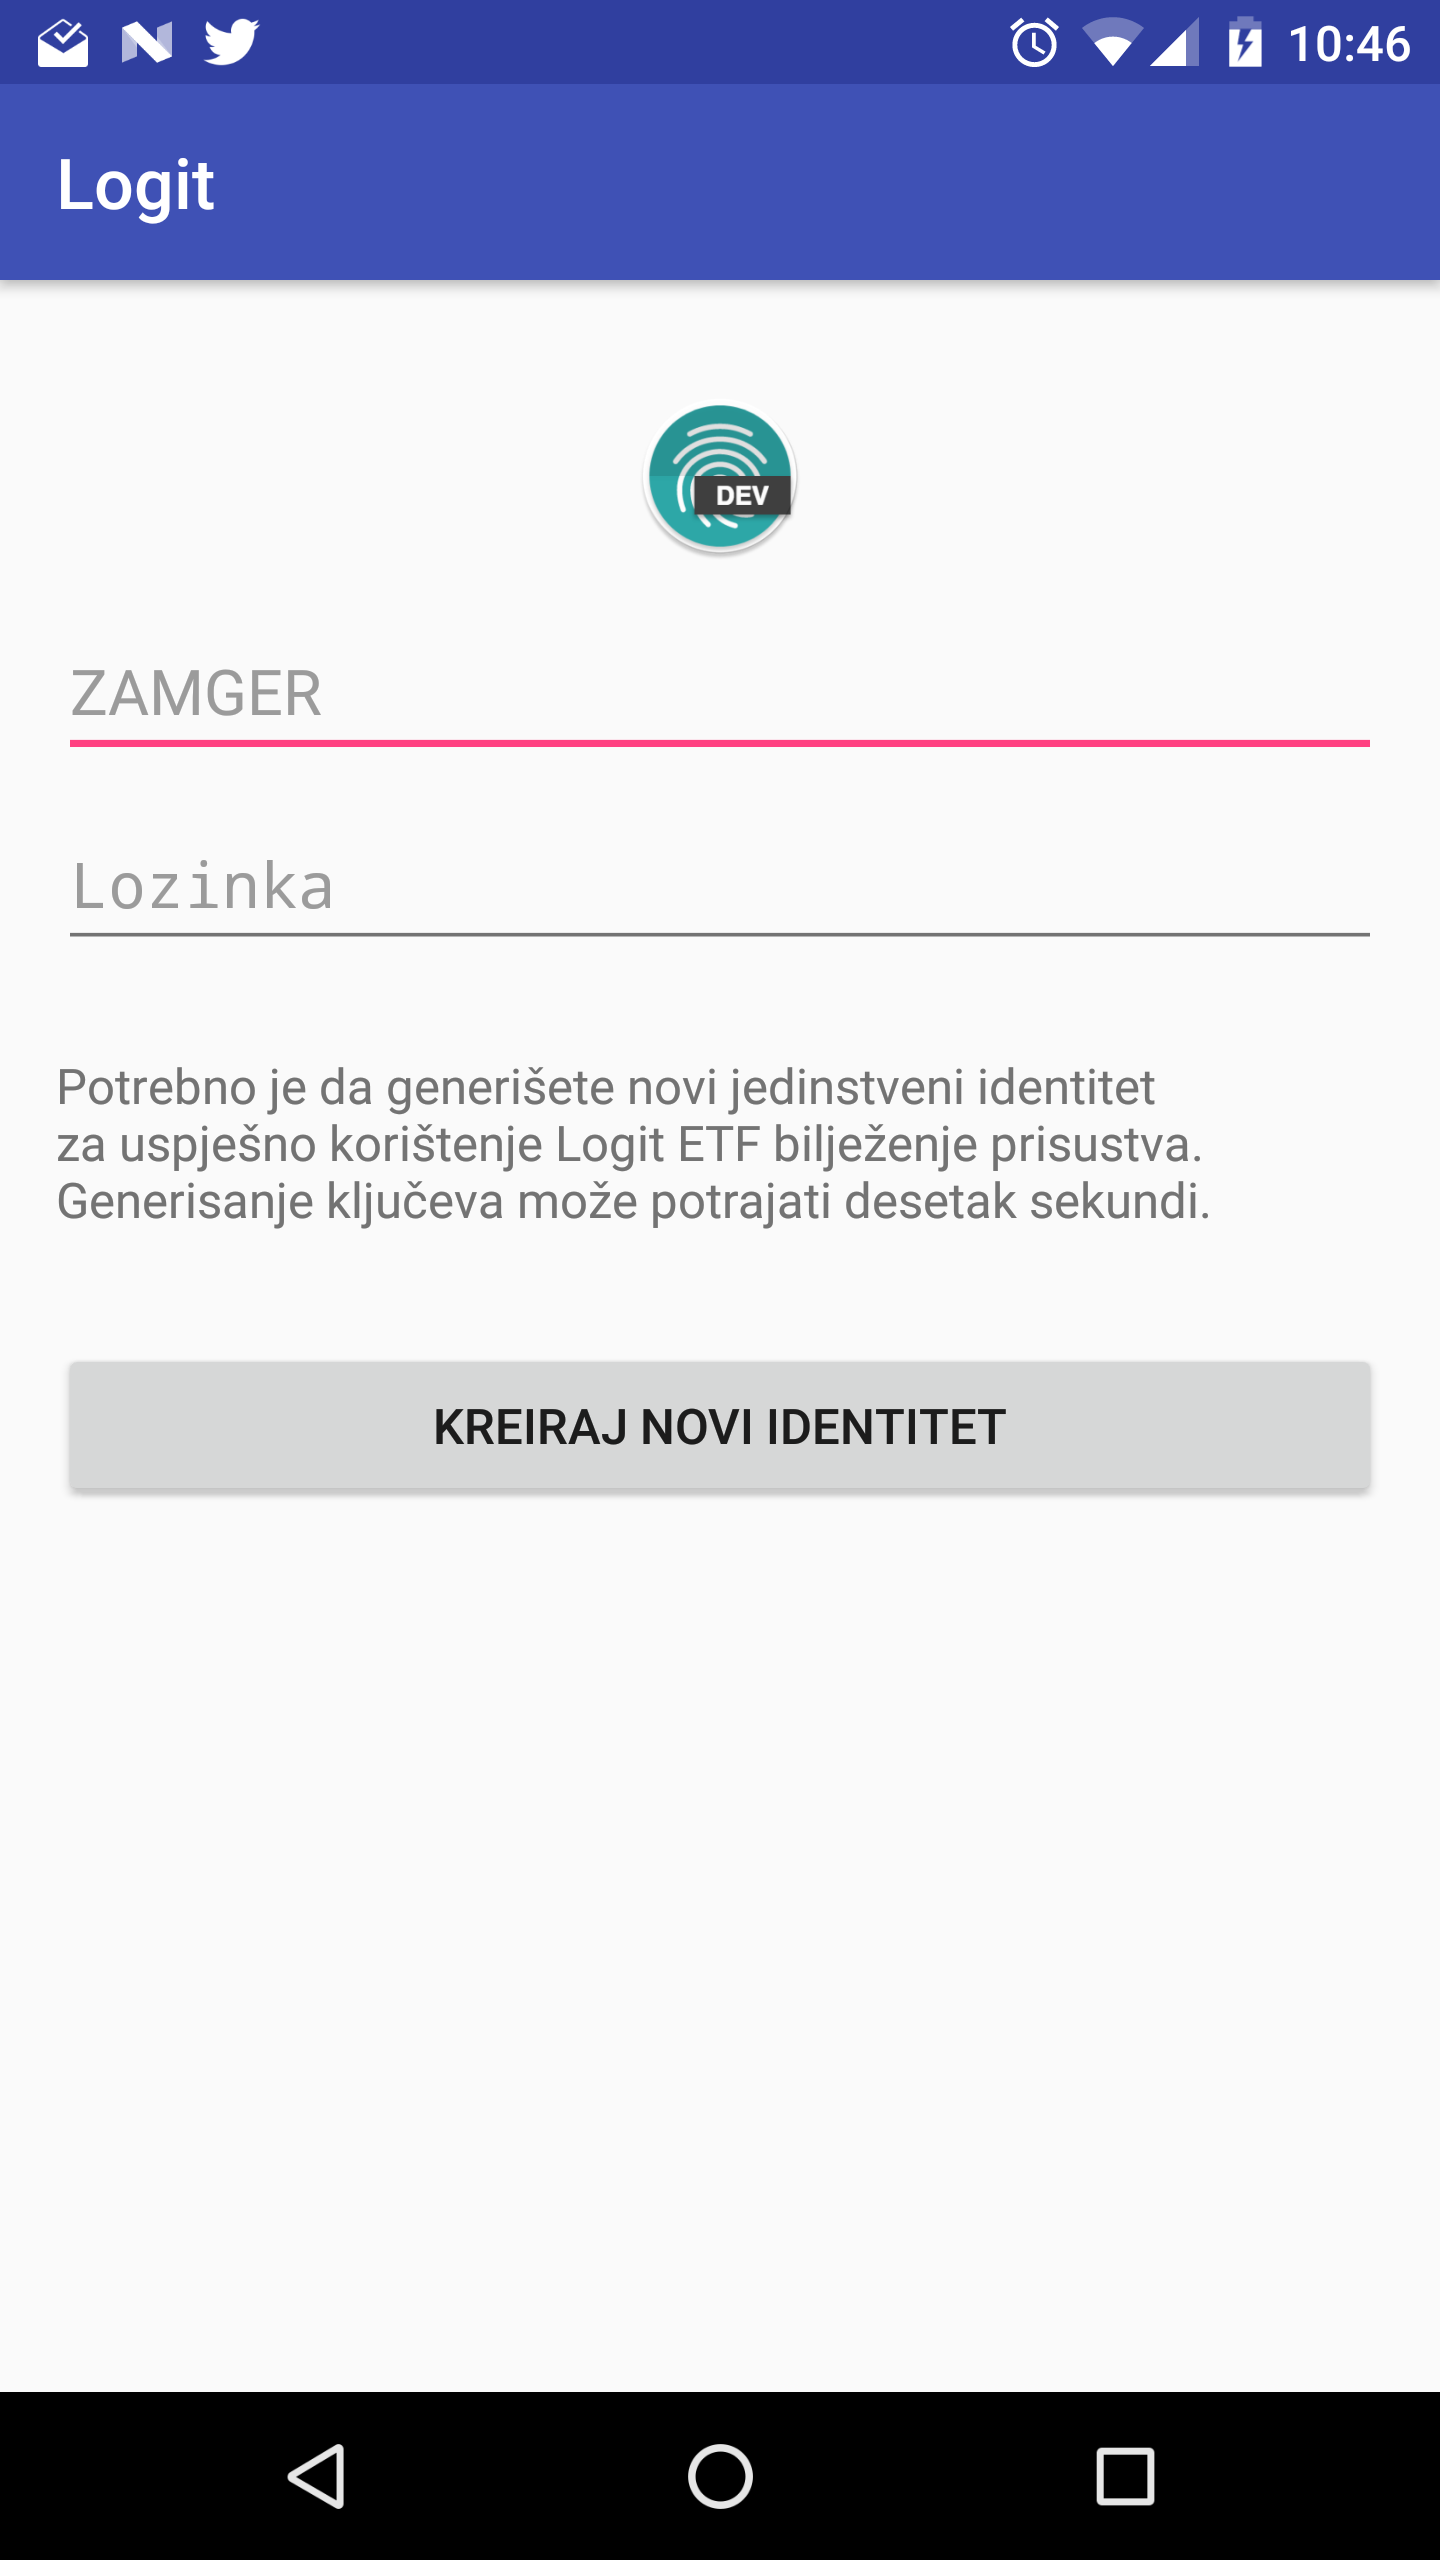
\includegraphics[width=0.45\textwidth]{material/00-login}
    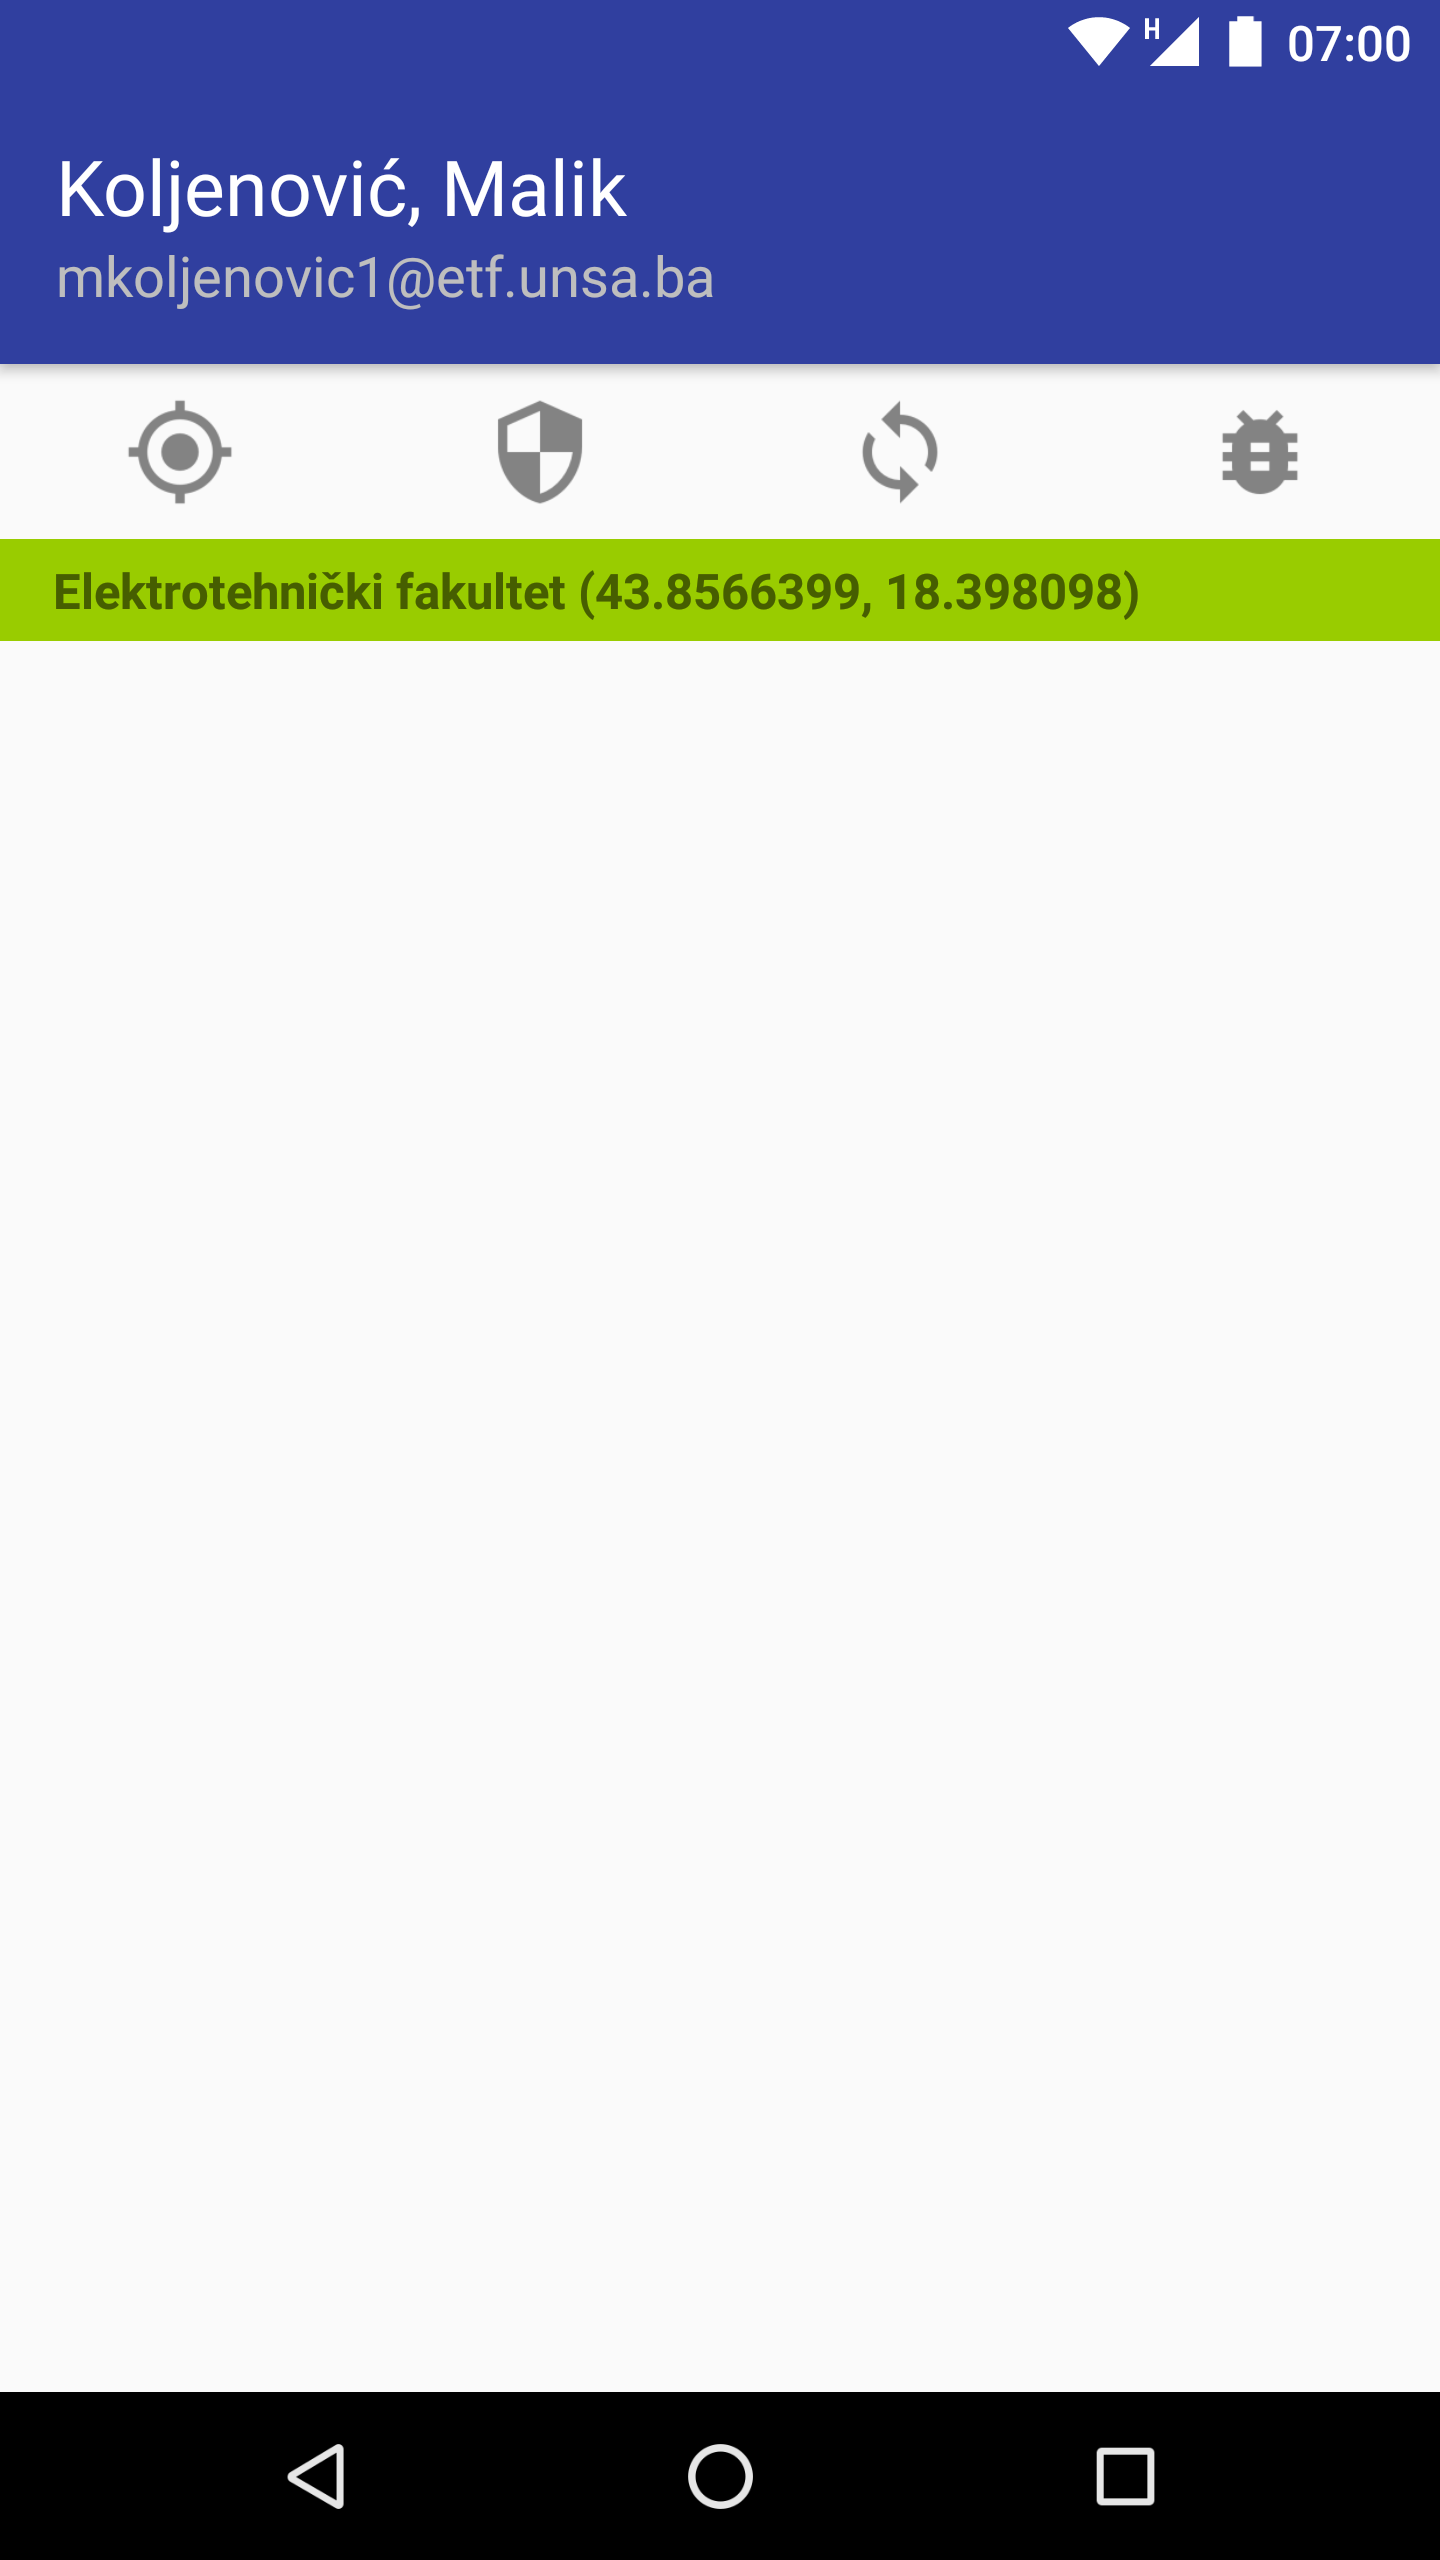
\includegraphics[width=0.45\textwidth]{material/01-attendance}
    \caption{Logit UI Android prikaz korisničkog interfejsa}
\end{figure}
%	\chapter{Pregled korištenih tehnologija} \label{chapter:tech}

\section{NFC \textit{(en. near-field communication)}}
NFC skup protokola omogućava uspostavu komunikacijskog kanala između dva uređaja koji se nalaze u neposrednoj blizini jedan drugog (1-4 cm) i razmjenu podataka između njih\cite{NFCProtocol}. Komunikacija se odvija na način da MASTER uređaj osluškuje signal na prijemniku i u slučaju detektovanje SLAVE signala uređaja pošiljaoca, propisanog istim standardom zaprima podatke i vrši obradu nad njima, komunikacija se u većini slučajeva odvija jednosmjerno kratkim standardiziranim porukama (NDEF), no moguće je ostvariti i half-duplex komunikaciju između uređaja, kao i razmjenu nestandardnih poruka, u kojem slučaju se sam korisnik mora pobrinuti za implementaciju kompletnog komunikacijskog protokola. Potpuni detalji implementacija dati su u referencama relevantnih standarda u nastavku tehničkog pregleda, odličnu sintezu detalja i implementacije daju Igoe, Coleman i Jepson\cite{Igoe2014}.
\subsection{NXP NTAG216}
U cilju zadovoljenja postavljenih funkcionalnih zahtjeva bilo je neophodno odabrati NFC Tag platformu koja će odrediti relevantne standarde pohrane binarnih podataka na uređajima kao i pripadajuće komunikacijske protokole, također dodatno su postavljeni zahtjevi ekonomičnosti implementacije i kompatibilnosti sa postojećim čitačima. Uzimajući u obzir nabrojane kriterije odabrana je platforma NTAG216 proizvođača NXP Semiconductors\cite{NTAG216} bazirana na NFC Forum Tag tipu 2 i ISO/IEC14443 Tip A specifikaciji\cite{NFCTag2}\cite{ISO14443}. 

\paragraph*{}
Mogućnosti navedene platforme dostatne su za ispunjenje navedenih funkcionalnih uslova, a pružaju i neke dodatne sigurnosne mehanizme - poput neizmjenjivog jedinstvenog serijskog broja svakog taga (Tag UID) potpisanog kriptografskim ključem proizvođača, navedena funkcionalnost nije implementirana u predstavljenom rješenju jer se bazira na zaštićenoj NXP tehnologiji i nije kompatibilna sa HCE emulacijom, no umnogome može doprinijeti ukupnoj sigurnosti fizičkih Tag čipova u slučaju produkcijske implementacije rješenja. U nastavku je data proizvođačka lista izdvojenih funkcionalnosti NTAG216:

\begin{itemize}[noitemsep]
    \item 7-bajtni UID programiran od strane proizvođača za svaki tag
    \item mogućnost jednokratnog programiranja i zaključavanja taga za dalje izmjene
    \item mogućnost read-only zaključavanja taga
    \item potpis originalnosti baziran na kriptografiji eliptičnih krivih
    \item zaštita memorijskih operacija 32-bitnom lozinkom
\end{itemize}

\paragraph*{}
Proces emulacije taga svodi se na što vjerniju reprezentaciju memorijskog prostora fizičkog uređaja u skadu sa relevantnim standardima, a opcionalno i dodatnih nestandardnih funkcionalnosti u vidu komunikacijskog protokola za korištenje naprednih funkcionalnosti date platforme. Kao minimum neophodan za standardnu komunikaciju NDEF porukama potrebno je emulirati generičko zaglavlje u obliku \textit{CC - capability container} i potpun zapis same NDEF poruke unutar korisničkog memorijskog prostora, potpun prikaz organizacije memorije NTAG216 platforme dat je na slici \ref{fig:ntag_mem}\cite{NTAG216}. Za emulaciju nestandardnih dijelova, poput zaštite čitanja korisničkog memorijskog prostora lozinkom ili emulaciju serijskog broja, za svaku različitu platformu neophodno je implementirati komunikacijski protokol u skladu sa proizvođačkom specifikacijom.

\begin{figure}[H]
    \centering
    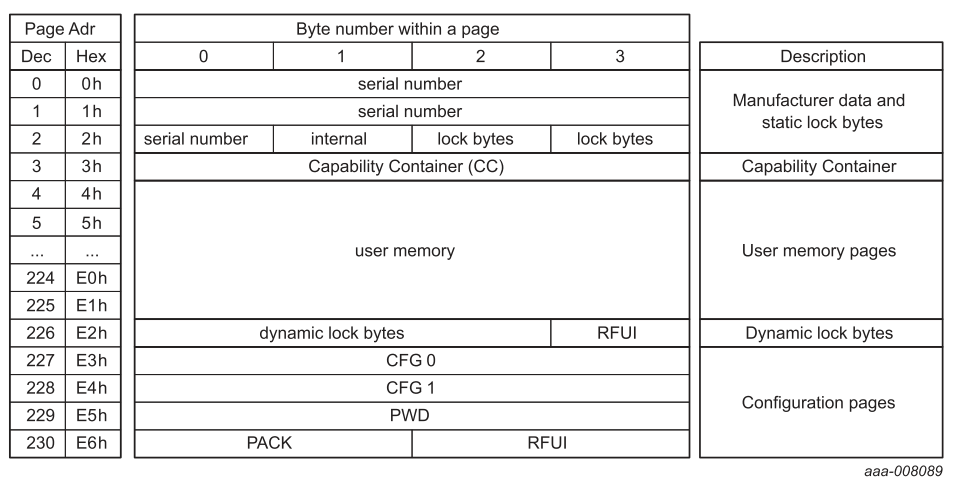
\includegraphics[width=1\textwidth]{material/ntag216-memory}
    \caption{NTAG216 organizacija memorije}
    \label{fig:ntag_mem}
\end{figure}

\subsection{NDEF \textit{(en. NFC Data Exchange Format)}}
NDEF specifikacija definiše \textbf{format enkapsulacije poruke} za razmjenu informacija između dva NFC uređaja. NDEF je lagan binarni format poruke i može se koristiti za enkapsulaciju jednog ili više aplikacijski-definisanih tereta \textit{(en. payload)} raznih vrsta i veličina unutar jedne NDEF poruke. Svaki teret opisan je od strane tipa, dužine i opcionalnog identifikatora. Identifikatori tipa mogu biti URI, MIME media tipovi, ili NFC-specifični tipovi. NDEF je striktno \textbf{format} poruke i ne poznaje pojam konekcije ili logičkog kola.\cite{NDEF}

\paragraph*{}
Neki od ciljeva koje NDEF nastoji da ispuni:
\begin{itemize}[noitemsep]
    \item enkapsulacija dokumenata i binarnih objekata, slika etc.
    \item enkapsulacija podataka nepoznate dužine, npr. stream-a podataka
    \item agregacija srodnih sadržaja unutar jedne poruke
    \item kompaktna enkapsulacija malih datagrama
\end{itemize}

\subsection{HCE \textit{(en. Host card emulation)}}
HCE je metod emuliranja virtuelnog identifikacijskog modula korisnika, u osnovi to je način zaobilaska hardverskih ograničenja (\textit{en. hack, workaround}) koja onemogućavaju direktan pristup SIM (\textit{en. Subscriber Identification Module}) modulu kod mobilnih telefonskih uređaja\cite{elenkov_2012}, ovakvo rješenje vuče korijene iz ekonomske realnosti sektora mobilnih komunikacija i kartičnog plaćanja, koja se najpreciznije može okarakterisati kao oligopol, naime Google je nastojao integrisati SIM karticu unutar Android operativnog sistema u vidu eSE (\textit{en. embedded Secure Element}) korištenjem već postojeće SIM kartice operatera a u svrhu razvoja Google Wallet rješenja, no to nije odgovaralo operaterima i odbili su suradnju, nakon toga Google iznalazi alternativne načine rješenja problema poput HCE\cite{randomoracle_2014}.

\paragraph*{}
HCE na Android OS radi, kako i naziv govori u CE (\textit{en. Card Emulation}) SLAVE modu, gdje se na svaki BUMP sa NFC čitačem odašilju pripremljeni podaci. Podaci koji se pri tome šalju moraju pratiti standard kartice koju žele emulirati i najčešće se vrši prijenos dokumenta ili datagrama unutar jednog ili više NDEF paketa. Logit koristi pristup prijenosa JSON formatiranog SPIM objekta \texttt{plain/text} unutar jednog NDEF paketa. Radi se o konceptu sa mnoštvom implementacijskih detalja, više detalja dostupno je u službenoj dokumentaciji\cite{androidhce_2018}, dok su izvrstan logički prikaz sa primjerima dali Coskun, Oz, Ozdenizci\cite{coskunAndroid}\cite{coskunNFC}, kao i Elenkov\cite{Elenkov2015} u znatno ažurnijem izdanju.

\section{Ostalo}
Dodatno koristi se Android arhitektura za dobavljanje geolokacije\cite{geoa} uz reverzno geokodiranje od strane OpenStreetMap Nominatim projekta\cite{nominatim}. Za potpisivanje i enkripciju korisničkih podataka koristi se RSA\cite{rivest1978method} kriptografija sa 2048 bit ključem. LAPI je Python flask API, kompletan listing koda dostupan je na GitHub u repozitorijima \texttt{koljenovic/logit} i \texttt{koljenovic/logit-node}.
%	\chapter{Izdvojeni detalji implementacije}
Detalji izdvojeni u ovom poglavlju ključni su za razumijevanje sigurnosnog modela aplikacije, sa tog aspekta posebno su zanimljiva dva objekta, \texttt{Attendance} i \texttt{Session}, koji u osnovi predstavljaju proširene kriptografski potpisane SPIM i SESS objekte.

\section{Podatkovni i kriptografski primitivi}
\subsection{SPIM paket}
Spim u širem smislu predstavlja vremensko-lokacijski objekat (\textit{en. SPace-tIMe}), koji korištenjem kriptografske obrade poprima karakteristike lokacijskog dokaza. Izvor za formiranje SPIM objekta sastoji se iz korisničkog imena studenta, geografske širine, geografske dužine i trenutnog vremena na studentovom mobilnom uređaju. Ovako komponovan objekat predstavlja implementaciju lokacijskog dokaza u užem smislu i koristi se dalje kao osnovni podatkovni primitiv za dalju kriptografsku obradu.

\inputminted{text}{material/logit_tag.txt}

\paragraph*{}
Navedene vrijednosti stringova korisničkog imena studenta, geografske širine, geografske dužine i trenutnog vremena se lančaju u jedan string izloženim redoslijedom i takav string se potpisuje korištenjem RSA kriptografije, tako potpisan paket u obliku JSON objekta (prikazan u listingu iznad) šalje se na profesorski master uređaj, gdje se dodaju podaci sesije, u vidu jedinstvenog identifikatora sesije (SID), te se potpisano studentsko prisustvo obilježava jedinstvenim heksadecimalnim identifikatorom AID izvedenim iz potpisa prisustva putem SHA256 hash funkcije, navedene vrijednosti, SID i AID se lančaju u jedan binarni string i potpisuju od strane profesora (CONFSIG), naknadno se na iz SHA256 hash vrijednosti CONFSIG profesorskog potpisa formira finalni identifikator potvrde prisustva CID, time se završava kriptografsko osiguravanje valjanosti prisustva u smislu SPIM objekta.

\begin{figure}[H]
    \centering
    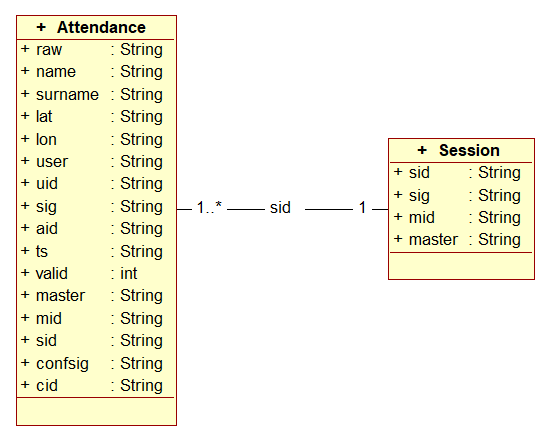
\includegraphics[width=0.6\textwidth]{material/classmodel}
    \caption{Dijagram klasa SPIM i SESS objekata}
\end{figure}
\begin{description}[align=right,labelwidth=2cm,noitemsep]
    \item [raw] serijalizirana string JSON verzija objekta
    \item [name] ime studenta
    \item [surname] prezime studenta
    \item [lat] geografska širina student
    \item [lon] geografska dužina student
    \item [user] ZAMGER korisničko ime studenta
    \item [uid] User ID - SHA2 hex hash javnog ključa studenta
    \item [sig] hex potpis SPIM-a (user:lat:lot:ts)
    \item [aid] Attendance ID - hex SHA2 hash \texttt{sig} potpisa
    \item [ts] vrijeme na studentovom uređaju
    \item [valid] validation cache
    \item [master] ZAMGER korisničko ime profesora
    \item [mid] Master ID - SHA2 hex hash javnog ključa profesora
    \item [sid] Session ID - identifikator profesorove sesije
    \item [confsig] Master Conf. profesorov hex potpis (sid:aid)
    \item [cid] Confirmation ID - SHA2 hex hash confsig-a
\end{description}

\paragraph*{}
Fizički predstavljen opisani SPIM objekat manji je od 1 KB te je pored brzog NFC isl. elektronskog transfera moguće izvršiti prenos alternativnim metodama, kao posebno pogodna čini se QR kod reprezentacija\cite{soon2008qr} i prenos, koja može biti vrlo korisna u slučaju da nijedan od uređaja ne posjeduje NFC modem. Navedeni modus nije implementiran u aplikaciji i dat je kao sugestija zaobilaženja hardverskih ograničenja, primjer QR oblika ranije datog SPIM objekta prikazan je na slici \ref{img:qr}.

\paragraph*{}
Dati QR prikaz je čitljiv ali je vidno uočljiva gustina zapisa koja može predstavljati problem u slučaju lošije kvalitete medija prikaza, u tom slučaju, kompletan SPIM paket moguće je značajno smanjiti zamjenom korištenog RSA kriptosistema za kriptosistem baziran na eliptičnim krivim, budući da su ključevi korišteni u tom slučajnu znatno kraći\cite{atmelecc}, dužina navedenog potpisa bila bi smanjena sa 512 na minimalno 71 bajt\cite{cheneau2009ecc} navedeni pristup nije prihvaćen u okviru ovog rada zbog povećanja kompleksnosti pokaznog sistema, no praktična implementacija moguća je bez većih programskih izmjena.

\begin{figure}[H]
    \centering
    \begin{subfigure}{.5\textwidth}
        \centering
        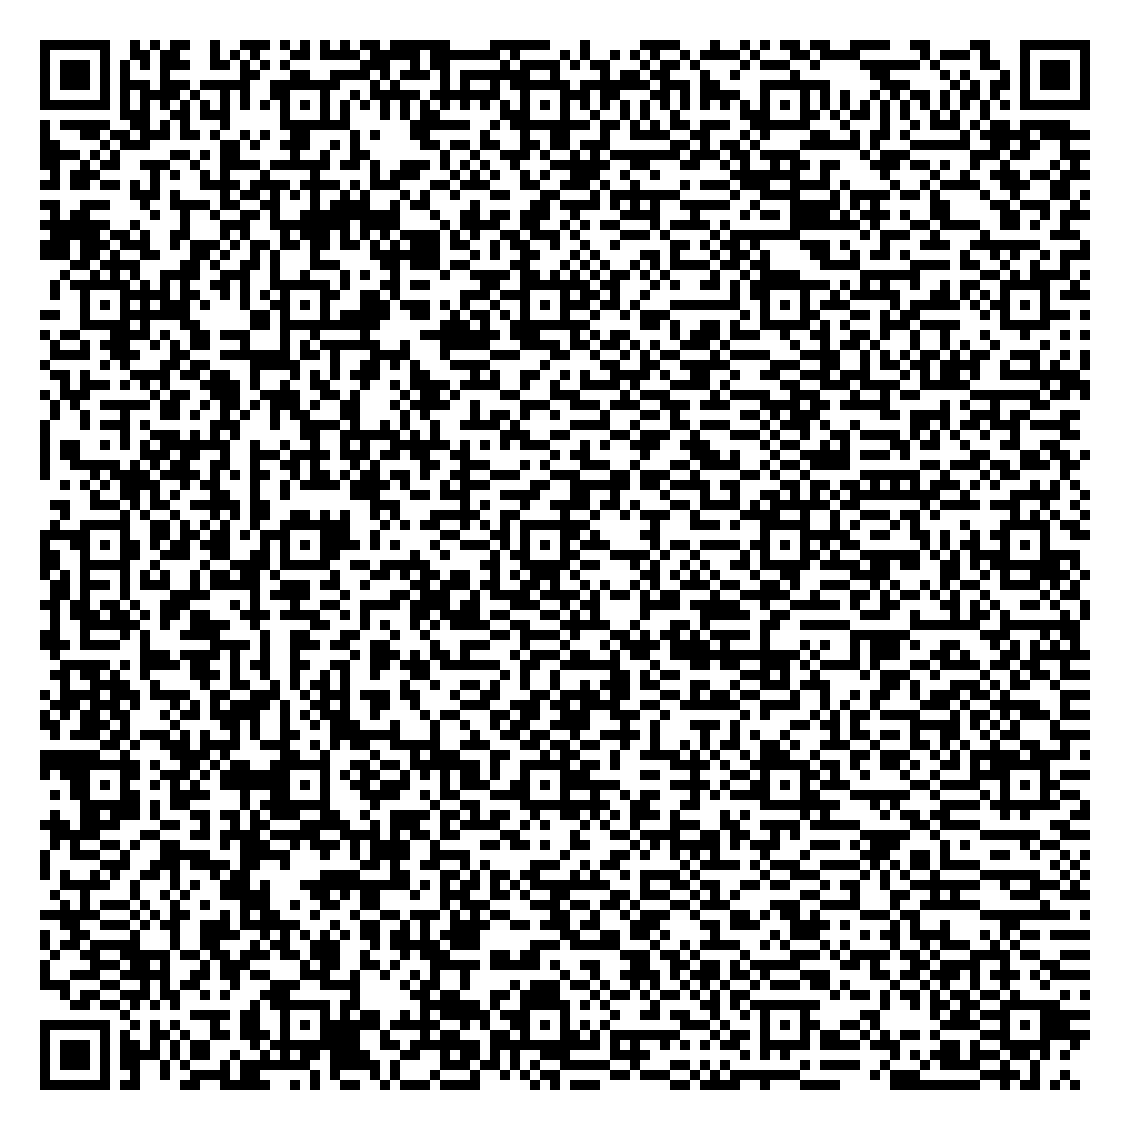
\includegraphics[width=.8\textwidth]{material/logit_qr}
        \caption{oblik korištenjem RSA potpisa}
        \label{img:qr_rsa}
    \end{subfigure}%
    \begin{subfigure}{.5\textwidth}
        \centering
        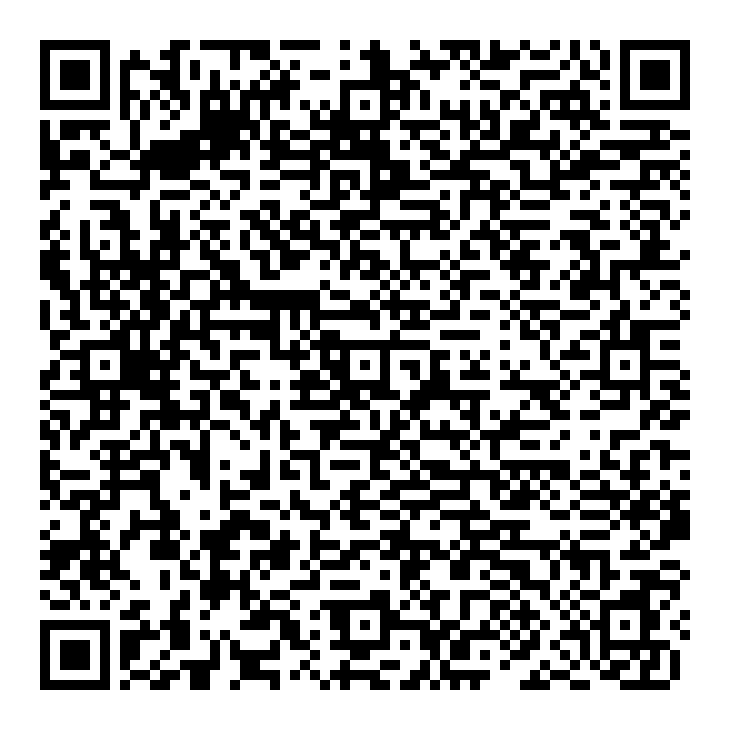
\includegraphics[width=.8\textwidth]{material/logit_qr_ec}
        \caption{oblik korištenjem ECC potpisa}
        \label{img:qr_ecc}
    \end{subfigure}
    \caption{QR oblik SPIM objekta}%
    \label{img:qr}
\end{figure}

\subsection{SESS paket}
Dodatno se za SESS objekat prilikom finaliziranja sesije na LAPI serveru vrši prikupljanje svih CID potpisa koji pripadaju datoj sesiji, te se CID vrijednosti ulančane hronološkim redoslijedom potpisuju LAPI ključem koji se nalazi samo na LAPI hardverskom uređaju, stoga je sigurnost LAPI servera od ključne važnosti za sigurnost ukupnog sistema. Ovako potvrđena sesija ne može biti naknadno mijenjana, lažirana ili porečena izvan LAPI izvršnog okruženja.

\cleardoublepage
\section{Pregled implementacije}
\subsection{MainActivity}
Nakon prvobitnog pokretanja aplikacije a za daljnje uspješno korištenje neophodno je izvršiti autentifikaciju korisnika putem nekog već postoječeg korisničkog repozitorija, te generisati pripadajući virtualizirani sigurni element. Navedene aktivnosti izvršavaju se unutar \texttt{MainActivity} glavnog početnog prozora Logit aplikacije, prikaz relevantnog dijela koda za generisanje virtualiziranog sigurnog elementa dat je u listingu ispod.

\begin{minted}{python}
    KeyPairGenerator kpg = KeyPairGenerator.getInstance(
            "RSA", "AndroidKeyStore");
    Calendar start = Calendar.getInstance();
    Calendar end = Calendar.getInstance();
    end.add(Calendar.YEAR, 1);

    KeyPairGeneratorSpec spec =
            new KeyPairGeneratorSpec.Builder(this).setAlias("etf_logit_" + ts)
                    .setKeySize(2048)
                    .setSubject(new X500Principal("CN=users.etf.ba"))
                    .setSerialNumber(BigInteger.valueOf(tsLong))
                    .setStartDate(start.getTime()).setEndDate(end.getTime()).build();

    kpg.initialize(spec);

    KeyPair kp = kpg.generateKeyPair();

    KeyStore ks = KeyStore.getInstance("AndroidKeyStore");
    ks.load(null);
\end{minted}

\paragraph*{}
Sigurnosni element generisan kao u primjeru iznad dalje se pohranjuje na korisničkom uređaju, gdje privatni dio nikada ne napušta uređaj i dostupan je isključivo Logit aplikaciji putem Android KeyStore providera. Javni dio se koristi kao dio identifikatora korisnika, te se dodatno pohranjuje i na Logit API korisnički repozitorij za potrebe identifikacije i verifikacije potpisa lokacijskog paketa.

\subsection{LogitAPDUService}
Ekstenzija Androidovog native interfejsa \texttt{HostApduService} koji za instaliranu aplikaciju sa \texttt{android.permission.BIND\_NFC\_SERVICE} permisijom vrši pokretanje HCE emulatora prilikom svakog starta operativnog sistema, emulator se u ovom slučaju ponaša kao generički NFC NTAG sa korisnički programiranom memorijom u obliku NDEF poruke koja prenosi jedinstveni potpisan studentski lokacijski dokaz. Navedena servisna komponenta aplikacije aktivna je svaki put dok je i ekran uređaja aktivan ili dok korisnik sam ne zaustavi pripadajući servis. Navedene funkcionalnosti postižu se uključivanjem dijela koda datog u nastavku unutar \texttt{<application>} direktive manifest fajla.

\begin{minted}{python}
    <service
        android:name=".LogitApduService"
        android:permission="android.permission.BIND_NFC_SERVICE">
        <intent-filter>
            <action android:name="android.nfc.cardemulation.action.HOST_APDU_SERVICE" />

            <category android:name="android.intent.category.DEFAULT" />
        </intent-filter>

        <meta-data
            android:name="android.nfc.cardemulation.host_apdu_service"
            android:resource="@xml/apduservice" />
    </service>
\end{minted}

\paragraph*{}
Nadalje \texttt{LogitAPDUService} sadrži logiku za ispravno konstruisanje i formatiranje NDEF paketa\cite{tindef} lokacijskog dokaza i njegovo potpisivanje, te ostalu neophodnu kriptografsku obradu. U nastavku će biti dat prikaz kompletnog servisa sa komentarima relevantnih dijelova.

\begin{minted}{python}
    final static int APDU_INS = 1;
    final static int APDU_P1 = 2;
    final static int APDU_P2 = 3;
    final static int APDU_SELECT_LC = 4;
    final static int APDU_READ_LE = 4;
    final static int FILEID_CC = 0xe103;
    final static int FILEID_NDEF = 0xe104;
    final static byte INS_SELECT = (byte) 0xa4;
    final static byte INS_READ = (byte) 0xb0;
    final static byte INS_UPDATE = (byte) 0xd6;
    final static byte P1_SELECT_BY_NAME = (byte) 0x04;
    final static byte P1_SELECT_BY_ID = (byte) 0x00;
    final static int DATA_OFFSET = 5;

    final static byte[] DATA_SELECT_NDEF = {(byte) 0xd2, (byte) 0x76, (byte) 0x00, (byte) 0x00, (byte) 0x85, (byte) 0x01, (byte) 0x01};
    final static byte[] RET_COMPLETE = {(byte) 0x90, (byte) 0x00};
    final static byte[] RET_NONDEF = {(byte) 0x6a, (byte) 0x82};
    final static byte[] FILE_CC = {
            (byte) 0x00, (byte) 0x0f,       // CCLEN - CC container size
            (byte) 0x20,                    // Mapping version
            (byte) 0x04, (byte) 0xff,       // MLe - max. read size
            (byte) 0x08, (byte) 0xff,       // MLc - max. update size

            // TLV Block (NDEF File Control)
            (byte) 0x04,                    // Tag - Block type
            (byte) 0x06,                    // Length
            (byte) 0xe1, (byte) 0x04,       // File identifier
            (byte) 0x04, (byte) 0xff,       // Max. NDEF file size
            (byte) 0x00,                    // R permission
            (byte) 0x00,                    // W permission
    };
\end{minted}

\paragraph*{}
Deklariše konstantne vrijednosti brojnih dijelova neophodnih za kontrukciju standardne NDEF poruke, između ostalog capability fajl koji predstavlja svojevrsno zaglavlje NDEF paketa.

\paragraph*{}
Metoda generateSignature instancira lokacijske servise i vrši konstukciju paketa lokacijskog dokaza kao i kriptografskih primitiva neophodnih za potpisivanje istog. Za konstrukciju lokacijskog dokaza neophodno je pribaviti trenutno vrijeme uređaja, to je prikazano u narednom dijelu koda.

\begin{minted}{python}
    Long tsLong = System.currentTimeMillis() / 1000;
    String ts = tsLong.toString();
    byte[] signature;
\end{minted}

\paragraph*{}
Nakon toga vršti se instanciranje i učitavanja Android KeyStore objekta koji sadrži korisnički par ključeva neophodnih za potpisivanje lokacijskog paketa.

\begin{minted}{python}
    KeyStore ks = KeyStore.getInstance("AndroidKeyStore");
    ks.load(null);
    KeyStore.ProtectionParameter pp = new KeyStore.PasswordProtection(null);
\end{minted}

\paragraph*{}
Nadalje iz \texttt{KeyStore} objekta učitava se najažurniji virtualizirani sigurnosni element.

\begin{minted}{python}
    Enumeration<String> aliases = ks.aliases();
    String alias = aliases.nextElement();
    Entry entry = ks.getEntry(alias, pp);
\end{minted}

\paragraph*{}
Zbog potrebe za što kompaktnijim prenosom podataka za sve vrijednosti gdje je to moguće generišu se hash preslikavanja koja se kasnije koriste za verifikaciju i pohranjivanje. Za potrebe generisanja hash vrijednosti instancirase SHA-256 \texttt{MessageDigest} objekat.

\begin{minted}{python}
    MessageDigest md = MessageDigest.getInstance("SHA-256");
\end{minted}

\paragraph*{}
Iz virtualiziranog sigurnog elementa dalje učitavamo korisnički certifikat sa javnim ključem, te za potrebe verifikacije identiteta heksadecimalnu reprezentaciju njegove hash vrijednosti pripremamo za uključenje u paket lokacijskog dokaza.

\begin{minted}{python}
    Certificate c = ks.getCertificate(alias);
    byte [] pubKey = c.getPublicKey().getEncoded();
    md.update(pubKey, 0, pubKey.length);
    byte [] pubKeyHash = md.digest();
    String pubKeyHashString = LogitApplication.toHext(pubKeyHash);
\end{minted}

\paragraph*{}
Zatim iz virtualiziranog sigurnog elementa korištenjem korisničkog privatnog ključa pripremamo objekat koji vrši potpisivanje lokacijskog paketa.

\begin{minted}{python}
    Signature s = Signature.getInstance("SHA256withRSA");
    s.initSign(((PrivateKeyEntry) entry).getPrivateKey());
    SharedPreferences userData = getSharedPreferences("UserData", 0);
\end{minted}

\paragraph*{}
Dio lokacijskog paketa koji je pokriven korisničkim digitalnim potpisom sadrži korisničko ime, lokacijske parametre geografske dužine i širine, te vrijeme uređaja u trenutku kreiranja digitalnog potpisa.

\begin{minted}{python}
    String sigPkg = userData.getString("user", "unknown") +
            ":" + location.getLatitude() +
            ":" + location.getLongitude() +
            ":" + ts;
\end{minted}

\paragraph*{}
Takav paket se potpisuje i bilježi se njegova SHA-256 preslikana vrijednost za potrebe verifikacije.

\begin{minted}{python}
    s.update(sigPkg.getBytes("UTF-8"));
    signature = s.sign();
\end{minted}

\paragraph*{}
Osnovni potpisani lokacijski paket se proširuje vrijednostima generisanih SHA-256 preslikavanja i osnovnim korisničkim podacima, te se prosljeđuje metodi createMessage koja formira standardizovan NDEF paket, takav spreman NDEF paket stavlja se na raspolaganje komponenti za prenos putem NFC protokola.

\begin{minted}{python}
    msg = "{\"lat\":\"" + location.getLatitude() +
            "\", \"lon\":\"" + location.getLongitude() +
            "\", \"ts\":\"" + ts +
            "\", \"sig\":\"" + LogitApplication.toHext(signature) +
            "\", \"uid\":\"" + pubKeyHashString +
            "\", \"name\":\"" + LogitApplication.toHext(userData.getString("name", "unknown").getBytes("UTF-8")) +
            "\", \"surname\":\"" + LogitApplication.toHext(userData.getString("surname", "unknown").getBytes("UTF-8")) +
            "\", \"user\":\"" + userData.getString("user", "unknown") + "\"}";

    NdefMessage ndef = createMessage(msg.getBytes("UTF-8"));
    byte[] ndefarray = ndef.toByteArray();

    mNdefFile = new byte[ndefarray.length + 2];

    mNdefFile[0] = (byte) ((ndefarray.length & 0xff00) >> 8);
    mNdefFile[1] = (byte) (ndefarray.length & 0x00ff);

    System.arraycopy(ndefarray, 0, mNdefFile, 2, ndefarray.length);

    logitApp.setMessage(mNdefFile);
\end{minted}

\subsection{processCommandApdu}
Budući da se u prikazanom slučaju vrši emulacija pasivnog NTAG uređaja, APDU servis se izvršava u slave modu i zaprima instukcije od strane master uređaja, neophodno je implementirati parser petlju i logiku za komunikaciju sa master uređajem, unutar koje se vrši prepoznavanje zadatih instrukcija i priprema adekvatan odgovor, navedena logika implementirana je unutar \texttt{processCommandApdu} metode. Kompletna logika emulacije tag uređaja svodi se na prosljeđivanje adekvatnog zaglavlja taga i READ FROM TO binarnog protokola za čitanje memorije koju šalje master, stoga glavninu navedene metode čini jedna switch petlja koja u skladu sa zadatom komandom vraća zaglavlje ili raspon bita emuliranog taga, u ovom slučaju sadržaj koji se emulira je prošireni lokacijski paket iznad. Detalje opisane metode možete pogledati u prilogu koda u dodatku.

\subsection{AttendanceActivity}
Za ostvarivanje pune funkcionalnosti aplikacije neophodna je bila implementacija master moda za prikupljanje i obradu NDEF paketa, u ovom slučaju korisničkih potpisa, enkapsuliranih u obliku potpisanog lokacijskog paketa. \texttt{AttendanceActivity} vrši navedenu funkcionalnost te dodatno vrši provjeru valjanosti potpisa i podataka korisničkih lokacijskih paketa. Verifikacija korisničkih lokacijskih paketa vrši se tako što se korisnički slave podaci o vremenu i lokaciji porede sa podacima o vremenu i lokaciji master uređaja, time se osigurava zaštita od napada lažiranja podataka, te bi za takvu vrstu prevare bila neophodna koluzija dva aktera suprostavljenih interesa, što znatno umanjuje vjerovatnoću takvih napada. Moguće je podesiti vrijednosti dozvoljenih odstupanja verifikacijskih parametara izmjenom koda za tu namjenu datog u nastavku.

\begin{minted}{python}
    final long timediff = System.currentTimeMillis() / 1000 - Long.parseLong(tmpAttn.getTs());
    final Location userLocation = new Location("MOCK");
    userLocation.setLatitude(Double.valueOf(tmpAttn.getLat()));
    userLocation.setLongitude(Double.valueOf(tmpAttn.getLon()));
    if (Build.VERSION.SDK_INT >= 23
            && ContextCompat.checkSelfPermission(that, android.Manifest.permission.ACCESS_FINE_LOCATION ) == PackageManager.PERMISSION_GRANTED
            && ContextCompat.checkSelfPermission(that, android.Manifest.permission.ACCESS_COARSE_LOCATION) == PackageManager.PERMISSION_GRANTED
            || Build.VERSION.SDK_INT < 23) {
        FusedLocationProviderClient mFusedLocatiionClient = LocationServices.getFusedLocationProviderClient(that);
        mFusedLocatiionClient.getLastLocation().addOnSuccessListener(new OnSuccessListener<Location>() {
            @Override
            public void onSuccess(Location location) {
                Float locdiff = userLocation.distanceTo(location);
                if (Math.abs(timediff) < 300) {
                    if (locdiff < 100) {
                        // Lokacija i vrijeme SLAVE uređaja su VALIDNI
                    } else {
                        Toast.makeText(that, "Greška: lokacije udaljene " + locdiff.intValue() + " metara.", Toast.LENGTH_LONG).show();
                    }
                } else {
                    Toast.makeText(that, "Greška: vrijeme nije tačno ili je TAG zastario.", Toast.LENGTH_LONG).show();
                }
\end{minted}

\paragraph*{}
Da bi se izbjegla obaveza reimplementiranja NDEF protokola za podatke primljene putem NFC podatkovnog interfejsa Android nudi predefinisani intent filter za direktnu manipulaciju NDEF poruka, te je za njegovo korištenje potrebno dodati ispod prikazani kod unutar manifest fajla Android aplikacije. Korištenjem ovog filtera programer kao rezultat uspješnog NFC prenosa dobija standardizovanu NDEF poruku spremnu za obradu. Ovaj interfejs se koristi unutar \texttt{AttendanceActivity}.

\begin{minted}{python}
<intent-filter>
    <action android:name="android.nfc.action.NDEF_DISCOVERED" />

    <category android:name="android.intent.category.DEFAULT" />

    <data android:mimeType="application/octet-stream" />
</intent-filter>
\end{minted}

\paragraph*{}
Ostatak koda unutar \texttt{AttendanceActivity} klase koristi se za prikaz i obradu elemenata korisničkog interfejsa master moda za prikupljanje korisničkih potpisa.
%	\chapter{Zaključak}
Aplikacija izrađena u okviru ovog rada zadovoljava zahtjeve navedene u postavci zadatka i pripadajućem opisu. Korištene su savremene kriptografske metode za implementaciju sigurnosno osjetljivih funkcionalnosti i osigurano je stabilno okruženje za neometano funkcionisanje aplikacije, dodatno je prema zahtjevima uspješno realiziran NFC komunikacijski interfejs između studentskih i instruktorskih mobilnih uređaja. U cilju lakšeg skaliranja težilo se je što više koristiti standardizovane tehnologije, posebno kada je u pitanju NFC, gdje je dodatno implementirana emulacija NTAG vrste taga kao NDEF medija, time je omogućeno da se sistem u budućnosti prilagodi stacionarnim NFC čitačima i korištenju samostalnih NFC tagova.

\paragraph*{}
Pokušana je pilot primjena sistema u saradnji sa nastavnim osobljem na predmetu "Tehnologije sigurnosti" u školskoj godini 2017/18. kojom prilikom je sačinjen spisak studenata i izvršene pripreme sistema. Navedena pilot primjena okončana je neuspješno zbog otvorenih sigurnosnih pitanja u integraciji sa postojećim sistemima, nedostatka resursa i nepostojanja pokusnog sistema pogodnog za projekte u ranoj fazi testiranja, stoga u cilju povećanja inovativnosti i razvoja novih usluga preporučuje se izrada pokusnih \textit{(en. staging)} sistema odvojenih od produkcijskog u okviru Elektrotehničkog fakulteta u Sarajevu.

\paragraph*{}
Tokom pripreme pilot primjene identifikovano je da značajan broj studenata ne posjeduje NFC omogućene mobilne uređaje, te su za njihove potrebe izrađene NTAG216 NFC token naljepnice, no primjena navedenih tokena uvjetovana je dodatnim istraživanjem i doradom Logit sistema za rad sa NTAG216 da bi osigurao isti ili viši nivo sigurnosnih garancija od onog koje pruža Android izvršno okruženje. Kao dodatna smjernica u istraživanju dat je prijedlog korištenja QR kodova za namjenu supstitucije u slučajevima nepostojanja tehničkih predispozicija za upotrebu sistema na strani korisnika, navedena tehnologija može dati dobre rezultate u praktičnoj primjeni i zavređuje dalji istraživački tretman.

\paragraph*{}
Krajnja težnja Logit rješenja je obuhvatanje cjelokupnog sistema autentifikacije i modeliranje relacija povjerenja u materijalnopravnom okruženju, kroz izradu proširive bazne platforme koja može obuhvatiti digitalizaciju mnoštva svakodnevnih administrativnih zadataka jedne institucije, sa tim ciljem daljnje istraživačke napore zavređuje usmjeriti ka razvoju stabilne PKI infrastrukture, kao i digitalizaciji vjerodostojnih institucionalnih registara poput registra ispita sa ciljem digitalizacije studentskog indeksa i srodnih dokumenata.
%	\begin{appendices}
%		\chapter{Funkcionalni opis Logit rješenja} \label{ch:man}
\begin{enumerate}
    \item \textbf{Uspostavite internet konekciju} prema uputama vašeg nastavnika.
    \begin{enumerate}
        \item potrebno je da na mreži bude dostupna Logit serverska aplikacija i certifikacijski repozitorij za uspješnu prijavu i korištenje, dostupnost možete provjeriti posjetom na \url{https://logit.mine.nu:5000}
    \end{enumerate}
    \item \textbf{Uključite lokacijske usluge} vašeg Android mobilnog uređaja.
    \begin{enumerate}
        \item detaljno uputstvo možete pronaći na \url{https://support.google.com/accounts/answer/3467281?hl=hr}
    \end{enumerate}
    \item \textbf{Omogućite NFC komunikaciju} na vašem Android mobilnom uređaju i \textbf{isključite Android Beam} uslugu za optimalan rad aplikacije.
    \begin{enumerate}
        \item \texttt{Settings > NFC > Enable}
        \item \texttt{Settings > NFC > Android Beam > Disable}
        \item više detalja za navedene postavke pročitajte na \url{https://support.google.com/nexus/answer/2781895?hl=hr}
    \end{enumerate}
    \item Ukoliko niste, \textbf{omogućite sigurnosnu funkcionalnost zaključavanja vašeg ekrana}
    \begin{enumerate}
        \item Android OS nudi usluge integrisane sigurnosti mobilnih uređaja, te je Keystore funkcionalnost sigurnog pohranjivanja privatnih ključeva usko vezana za ostale sigurnostne postavke, stoga omogućite zaključavanje ekrana slijedeći uputstvo na \url{https://support.google.com/nexus/answer/2819522?hl=hr}
    \end{enumerate}
    \item Prihvatite poziv za alpha testiranje posjetom na \url{https://play.google.com/apps/testing/ba.unsa.etf.logit} i nastavite na Play Store te \textbf{instalirajte aplikaciju}
    \begin{enumerate}
        \item ukoliko vaš mobilni uređaj nije izlistan kao podržan obratite se vašem nastavniku i biti će vam izdat jedinstveni NFC Certifikat, koji ćete koristiti za bilježenje prisustva
    \end{enumerate}
    \item \textbf{Pokrenite Logit aplikaciju}
    \item \textbf{Unesite vaše ZAMGER korisničke podatke}, ovi podatci koriste se jednokratno za provjeru valjanosti identiteta prije generisanja vašeg para ključeva, vaša lozinka ne ostaje pohranjena na Logit sistem i prenosi se https kanalom prema ZAMGER servisu
    \item Aplikacija je spremna za korištenje i ne mora biti pokrenuta u prednjem planu za prijavu prisustva, \textbf{za optimalne rezultate} dovoljno je da upalite ekran vašeg Android uređaja na “lock screen” i prislonite na Android uređaj nastavnika.
    \item \textbf{Ukoliko želite koristiti aplikaciju u nastavničkom modu} i prikupljati prisustvo, dovoljno je da pokrenete Logit aplikaciju u prednjem planu te prislonite vaš uređaju studentskom uređaju u skladu sa korakom 8.
\end{enumerate}

%\pagebreak[4]
\section{Nastavnički način rada}
\paragraph*{}
Pokretanjem glavnog prozora Logit aplikacije ulazite u mod za prikupljanje studentskih potpisa prisustva. Ovaj zaslon podijeljen je na četiri komponente, opisi kako slijedi u nastavku.

\begin{figure}[H]
    \centering
    
\includegraphics[width=0.6\textwidth]{material/manual/01-head}
    \caption{Zaglavlje aplikacije prikazuje aktivnog korisnika}
\end{figure}

\begin{figure}[H]
    \centering
    
\includegraphics[width=0.6\textwidth]{material/manual/02-menu}
    \caption{Glavni izbornik, opisi funkcionalnosti u nastavku}
\end{figure}

\begin{description}[noitemsep,align=right,labelwidth=2cm]
    \item [Dugme 1] služi za ručno osvježavanje trenutne lokacije
    \item [Dugme 2] koristite za provjeru valjanosti ključeva korištenih pri potpisu
    \item [Dugme 3] sinhronizacija trenutne sesije na Logit server, svi potpisi se pohranjuju u jednu sesijsku cjelinu i brišu sa mobilnog uređaja (kreira se nova sesija)
    \item [Dugme 4] otvara e-mail klijent po izboru korisnika u cilju lakše prijave grešaka
\end{description}

\begin{figure}[H]
    \centering
    
\includegraphics[width=0.6\textwidth]{material/manual/03-geobar}
    \caption{Trenutno zabilježena lokacija korisničkog uređaja}
\end{figure}

\begin{figure}[H]
    \centering
    
\includegraphics[width=0.6\textwidth]{material/manual/04-attns}
    \caption{Ordinalno numerisan spisak prisutnih studenata}
\end{figure}
%		\chapter{LAPI model podataka}
%		\chapter{Logit API Dokumentacija}
%		\chapter{Izvorni kod}
\section{LAPI izvorni kod}
{\small Repo: \url{https://github.com/koljenovic/logit-node/}}
\begin{minted}{text}
.
├── Logit
│   ├── Logit
│   │   ├── __init__.py
│   │   ├── logit.db
│   │   └── static
│   └── logit.wsgi
├── README.md
└── README.md~
\end{minted}
\subsection{\small \url{__init__.py}}
\inputminted{python}{../logit-node/Logit/Logit/__init__.py}

\section{Android izvorni kod}
{\small Repo: \url{https://github.com/koljenovic/logit/tree/master/android/app/src/main}}
\begin{minted}{text}
.
├── AndroidManifest.xml
├── ic_launcher-web.png
├── java
│   └── ba
│       └── unsa
│           └── etf
│               └── logit
│                   ├── api
│                   │   └── LogitService.java
│                   ├── AttendanceActivity.java
│                   ├── AttendanceAdapter.java
│                   ├── LogitApduService.java
│                   ├── LogitApplication.java
│                   ├── MainActivity.java
│                   └── model
│                       ├── Attendance.java
│                       ├── Place.java
│                       ├── Session.java
│                       └── User.java
└── res
    ├── ---
    │ 
\end{minted}

\pagebreak[4]
\subsection{\small \url{AndroidManifest.xml}}
\inputminted{xml}{../logit/android/app/src/main/AndroidManifest.xml}

\subsection{\small \url{model/Attendance.java}}
\inputminted{java}{../logit/android/app/src/main/java/ba/unsa/etf/logit/model/Attendance.java}

\subsection{\small \url{model/Place.java}}
\inputminted{java}{../logit/android/app/src/main/java/ba/unsa/etf/logit/model/Place.java}

\subsection{\small \url{model/Session.java}}
\inputminted{java}{../logit/android/app/src/main/java/ba/unsa/etf/logit/model/Session.java}

\subsection{\small \url{model/User.java}}
\inputminted{java}{../logit/android/app/src/main/java/ba/unsa/etf/logit/model/User.java}

\subsection{\small \url{api/LogitService.java}}
\inputminted{java}{../logit/android/app/src/main/java/ba/unsa/etf/logit/api/LogitService.java}

\subsection{\small \url{AttendanceActivity.java}}
\inputminted{java}{../logit/android/app/src/main/java/ba/unsa/etf/logit/AttendanceActivity.java}

\subsection{\small \url{AttendanceAdapter.java}}
\inputminted{java}{../logit/android/app/src/main/java/ba/unsa/etf/logit/AttendanceAdapter.java}

\subsection{\small \url{LogitApduService.java}}
\inputminted{java}{../logit/android/app/src/main/java/ba/unsa/etf/logit/LogitApduService.java}

\subsection{\small \url{LogitApplication.java}}
\inputminted{java}{../logit/android/app/src/main/java/ba/unsa/etf/logit/LogitApplication.java}

\subsection{\small \url{MainActivity.java}}
\inputminted{java}{../logit/android/app/src/main/java/ba/unsa/etf/logit/MainActivity.java}
%	\end{appendices}
%	
%	\bibliographystyle{ieeetr}
%	\bibliography{main}
%\end{document}

% iskljucivanje broja strane iz Sadrzaja, Popisa slika i Popisa tabela
\AtBeginDocument{\addtocontents{toc}{\protect\thispagestyle{empty}}}
\AtBeginDocument{\addtocontents{lof}{\protect\thispagestyle{empty}}}
\AtBeginDocument{\addtocontents{lot}{\protect\thispagestyle{empty}}}

\addto\captionscroatian{
  \renewcommand{\bibname}{Literatura}
  \renewcommand{\tablename}{Tabela}
  \renewcommand{\nomname}{Popis oznaka}
  \renewcommand{\indexname}{Indeks pojmova}
  \renewcommand{\lstlistingname}{Program}
  \renewcommand{\glossaryname}{Indeks pojmova}
  \renewcommand{\acronymname}{Indeks pojmova} 
}

%\addto\captionscroatian{\renewcommand{\listtablename}{Popis tabela}}
\addto\captionscroatian{\renewcommand\appendixname{Prilog}}
\addto\captionscroatian{\renewcommand\appendixpagename{Prilozi}}
\renewcommand\appendixtocname{Prilozi}

\makeindex
\makenomenclature
\newglossaryentry{LAPP}
{name={LAPP}, description={Logit višekomponentna aplikacijska platforma}}

\newglossaryentry{UI}
{name={UI}, description={Android komponente LAPP platforme}}

\newglossaryentry{LAPI}
{name={LAPI}, description={Logit API, Python serverska aplikacija, komponenta LAPP platforme}}

\newglossaryentry{ATTN}
{name={ATTN}, description={repozitorij potpisanih prisustva spremljen na LAPI}}

\newglossaryentry{CERT}
{name={CERT}, description={javni dio korisničkog kriptografskog ključa}}

\newglossaryentry{SSO}
{name={SSO}, description={\textit{(en. Single Sign On)} - politika autentifikacije korištenjem jedinstvenog repozitorija}}

\newglossaryentry{KEYS}
{name={KEYS}, description={jedinstveni set korisničkih RSA ključeva dužine 2048 bita}}

\newglossaryentry{DEVICE}
{name={DEVICE}, description={korisnički Android uređaj}}

\newglossaryentry{SPIM}
{name={SPIM}, description={\textit{(en. SPacetIME)} - lokacijski dokaz (JSON objekat, struktura podatka)}}

\newglossaryentry{HCE}
{name={HCE}, description={\textit{(en. Host card emulation)} softverska arhitektura koja omogućava virtualnu emulacija elektronskog identiteta}}

\newglossaryentry{M}
{name={M}, description={\textit{(en. master)} - Android UI komponenta pokrenuta na uređaju koji bilježi prisustvo}}

\newglossaryentry{S}
{name={S}, description={\textit{(en. slave)} - Android komponenta koja se izvršava u pozadini na uređaju čije se prisustvo bilježi}}

\newglossaryentry{BUMP}
{name={BUMP}, description={približavanje mobilnih uređaja, otvara jednosmjerni komunikacijski kanal u smijeru od slave (S) prema master (M) uređaju}}

\newglossaryentry{ISO14443A}
{name={ISO/IEC 14443 Tip A}, description={standard fizičkog sloja NFC komunikacijskog protokola}}

\newglossaryentry{NFC Forum Tag}
{name={NFC Forum Tag}, description={standardizovani format NFC taga}}

\newglossaryentry{NDEF}
{name={NDEF}, description={vrsta standardizovanog paketa korištena za NFC komunikaciju između uređaja}}

\newglossaryentry{NDEFMSG}
{name={NDEFMSG}, description={NDEF poruka koja sadrži vremensko-lokacijski dokaz potpisan od strane korisnika}}

\begin{document}
    \frontmatter
	\maketitle
    \afterpage{\blankpage}
\paragraph*{Abstract}
This thesis addresses the problem of large scale electronic attendance taking in university setting by presenting an Android based attendance taking application, based on immutable and non repudiable location proofs backed by RSA cryptography, utilizing NFC and HCE for ease of use, emulating NFC Forum Tag Type 4 it is also compatible with existing reader infrastructures. It also presents a general overview of the utilized techologies and select implementation details.

\paragraph*{Apstrakt}
Ova teza tretira problem masovnog elektronskog bilježenja prisustva u univerzitetskom okruženju izradom prijedloga aplikacija bazirane na Android platformi korištenjem neizmjenjivih i neporecivih vremensko-lokacijskih dokaza osiguranih korištenjem RSA kriptografije, te NFC i HCE tehnologija u cilju jednostavnosti upotrebe; emulirajući NFC Forum Tag Tip 4 kompatibilna je sa postojećim infrastrukturama čitača. Dat je i opšti pregled korištenih tehnologija i izdvojenih implementacijskih detalja.

\paragraph*{MSC Primary 68P25; Secondary 94A60;}
\paragraph*{Keywords:} NFC - near-field communication, HCE - host card emulation, security, Android, attendance, RSA, cryptography, NDEF, NTAG, geolocation, location proofs
    \pagebreak
%%%%%%%%%%%%%%%%%%%% POSTAVKA RADA %%%%%%%%%%%%%%%%%%%%%%%%%%%%%%%
\thispagestyle{plain}
\begin{flushleft}
\textbf{Elektrotehnički fakultet, Univerzitet u Sarajevu}\\
\textbf{Odsjek za računarstvo i informatiku}\\
\textbf{Vanr. prof. dr Saša Mrdović, dipl.ing.el.}\\

\textbf{Sarajevo, decembar 2016.}\\
\end{flushleft}

\begin{center}
\vspace{0.5cm}
{\Large Postavka zadatka završnog rada II ciklusa:}\\
\vspace{0.2cm}
{\large \textbf{Aplikacija za evidentiranje prisustva}}
\end{center}

\paragraph*{}
Potrebno je napraviti Android aplikaciju koja omogućava evidentiranje prisustva upotrebom NFC tehnologije. Aplikacija treba da bude jednostavna za upotrebu i zaštićena od zloupotreba.

\paragraph*{}
U okruženju u kom se većina komunikacija odvija elektronski za očekivati je da se i evidentiranje prisustva može raditi na ovaj način. Međutim, postoje otvorena pitanja pogodnosti i sigurnosti elektronskog evidentiranja. NFC može biti osnova za siguran i jednostavan sistem. Kako savremeni mobilni uređaji uglavnom imaju NFC oni mogu biti iskorišteni kao sredstvo prijavljivanja i vođenja evidencije bez potrebe za dodatnim karticama i čitačima.

\paragraph*{}
U radu je potrebno objasniti šta se podrazumjeva pod pojmom evidencija prisustva i koja su otvorena pitanja elektronskog vođenja ove evidencije. Potrebno je objasniti šta je NFC i kako radi. Potrebno je teoretski objasniti kako je moguće napraviti siguran elektronski sistem evidentiranja prisustva zasnovan na NFC koji je lak za upotrebu. U sklopu rada potrebno je napraviti praktičnu izvedbu sistema koji omogućava korisnicima koji imaju mobilne uređaje sa NFC da se pomoću njih registruju i potvrde prisustvo. Ovaj sistem treba biti zaštićen od zloupotreba. Prokomentarisati iskustva stečena tokom praktične realizacije i dati savjete za buduće izvedbe.

\vspace{0.5cm}
\textbf{Polazna literatura:}

\begin{itemize}
\item[] [1] V. Coskun, K. Ok, B. Ozdenizci, "Professional NFC Application Development for Android", Wrox, 2013
\item[] [2] T. Igoe, D. Coleman, B. Jepson, "Beginning NFC: Near Field Communication with Arduino, Android, and PhoneGap", O'Reilly Media, 2014
\item[] [3] J. Annuzzi Jr., L. Darcey, S. Conder, "Introduction to Android Application Development: Android Essentials", 4. izdanje, Addison-Wesley Professional, 2013.
\item[] [4] Ross Anderson, “Security Engineering", 2nd edition, Wiley, 2008.
\item[] [5] Bill Phillips, Brian Hardy, "Android Programming: The Big Nerd Ranch Guide", Big Nerd Ranch Guides, 2013.
\item[] [6] V. Coskun, K. Ok, B. Ozdenizci, "Near Field Communication (NFC): From Theory to Practice", Wiley, 2012
\end{itemize}

\begin{center}
\vspace{1cm}
\makebox[8cm]{\hrulefill} \\
Vanr. prof. dr Saša Mrdović, dipl.ing.el.\\
\end{center}






    %%%%%%%%%%%%%%%%%%%% POTPISI CLANOVA KOMISIJE %%%%%%%%%%%%%%%%%%%%
\pagebreak
\thispagestyle{plain}
\vspace{2cm}
\begin{center}
\textbf{\Large Potpisi članova Komisije za ocjenu i odbranu završnog rada II ciklusa}\\


\vspace{4cm}
\makebox[10cm]{\hrulefill} \\
Red. prof. dr Dženana Đonko, dipl.el.ing, \\
predsjednica komisije\\

\vspace{3cm}
\makebox[10cm]{\hrulefill} \\
Vanr. prof. dr Saša Mrdović, dipl.ing.el., \\
mentor i član komisije\\

\vspace{3cm}
\makebox[10cm]{\hrulefill} \\
Vanr. prof. dr Samir Omanović, dipl.el.ing, \\
član komisije

\end{center}

%    %%%%%%%%%%%%%%%%%%%% PREDGOVOR %%%%%%%%%%%%%%%%%%%%

\chapter*{Predgovor}

U predgovoru autor ima pravo da izrazi svoja lična uvjerenja i dojmove koji se vežu za sam rad. Najčešće se u predgovoru pišu zahvalnice svima koji su direktno ili indirektno pomogli prilikom pisanja rada (porodica, profesori i kolege itd.). 

Nadam se da će ovaj predložak za izradu završnog rada pomoći svim studentima Elektrotehničkog fakulteta u Sarajevu da napišu što bolje i kvalitetnije završne radove prvog, drugog ili trećeg ciklusa.

\vspace{1cm}
\begin{flushright}
\begin{tabular}{m{6cm}}
Nikola Tesla,\\
juli 2018.
\end{tabular}
\end{flushright}


  	\begin{center}
    \textsc{\LARGE Izjava o autorstvu}
\end{center}
\vfill
\paragraph*{}
Ja, \textbf{Malik (Zijad) Koljenović}, student Elektrotehničkog fakulteta, Univerziteta u Sarajevu, pod punom moralnom, materijalnom i krivičnom odgovornošću \textbf{izjavljujem} da je ovaj rad i pripadajući programski kod, pod naslovom \textsc{``Aplikacija za evidentiranje prisustva''} u potpunosti rezultat vlastitog istraživanja, gdje su korišteni sadržaji drugih autora (tekst, ilustracije, tabele etc.) jasno označeni pozivanjem na izvor.

\vfill

\noindent
\begin{flushright}
    \hspace{0.5cm} \makebox[2in]{\hrulefill} \\
    \textsc{Malik Koljenović, 984/2015}
\end{flushright}
\clearpage
  	
   	\tableofcontents
	\listoffigures
	%\listoftables
    \glsaddall
	\printglossaries
	
    \cleardoublepage % start new page
    \pagestyle{fancyplain} % puts headers/footers back on
    \fancyhf{}
    \lhead{\nouppercase{\fancyplain{}{\leftmark}}}
    \renewcommand{\chaptermark}[1]{\markboth{#1}{}}
    \renewcommand{\footrulewidth}{0.4pt} %draw foot line
    \lfoot{\slshape Koljenović, M., "Aplikacija za evidentiranje prisustva"}
    \rfoot{\thepage}
    \cfoot{}

    \mainmatter
	\chapter{Uvod}
Prodor digitalnih računara i komunikacijskih tehnologija u sve sfere ljudskog života i djelovanja, te dramatično povećanje broja korisnika interneta u posljednjoj deceniji nametnulo je mnoštvo novih društvenih i tehničkih izazova. Društveni izazovi najbolje su uočljivi kroz višedecenijsku debatu o privatnosti i vlasništvu nad ličnim podacima, samim time zadiru duboko u diskusiju o ljudskim pravima i identitetu sa jedne i često suprostavljenim komercijalnim interesima sa druge strane. Ukoliko se u tom kontekstu posmatra aktuelna EU uredba o zaštiti podataka\cite{gdpr} (\textit{en. GDPR}) postaje jasno da su digitalna tehnologija i komunikacije postale integralni dio društvene i emocionalno-psihološke realnosti\cite{Searle1995}, do te mjere da se digitalni tragovi smatraju dijelom nepovredivog identiteta osobe. Iz navedenog je jasno da se radi o institucionalizaciji jedne potpuno nove društveno-tehnološke paradigme unutar pravnih okvira Europske unije.

\paragraph*{}
Sa tehničke strane, dostignuća na poljima kriptografije, teorije mreža i novih komunikacijskih tehnologija, te njihova široka prihvaćenost otvorila su mogućnosti izrade računarskih sistema spremnih da odgovore na novonastale društvene izazove u okviru opisane nove paradigme. Pomenuti računarski sistemi kao dodatno izvršno okruženje imaju društveno-pravnu realnost te se u tim okvirima izvršavaju masovno, dobrovoljno, distribuirano i interaktivno\cite{Cahill2003} van centralizovanog računarskog izvršnog okruženja u smislu Von Neumannove arhitekture. Opisani sistemi mogu se okarakterisati kao sistemi potpomaganja (\textit{en. assist}), npr. kriptografski računarski sistem u domenu autentifikacije i autorizacija u novoj paradigmi postmatra se kao sistem računarski-potpomognutog povjerenja, ekvivalentno višem nivou apstrakcije.

\paragraph*{}
Registri u kontekstu društvenih institucija su elementarni mehanizam sistema povjerenja, sigurnosne karakteristike takvih institucionalnih registara stoga čine osnov istraživačkog interesa u domenu institucionalne sigurnosi. Napredni elektronski registri izrađeni korištenjem kriptografskih tehnika i savremenih komunikacijskih protokola za prikupljanje i obradu podataka omogućavaju poboljšanje njihovih sigurnosnih osobina, otvarajući nove načine primjene i stvarajući uslove za viši nivo društvenog razvoja i institucionalne efikasnosti, uz to pružaju i adekvatan odgovor na novonastale društvene izazove. Stoga, ukoliko se obezbijede i ispoštuju preduslovi izrade sigurnog sistema\cite{iso2013iso}, evidenciju prisustva u kontekstu naprednog elektronskog registara treba posmatrati i kao vremensko-prostorni dokaz određenog događaja, ovaj rad usmjeren je na izradu jednog takvog sistema računarski-potpomognutog povjerenja u obliku institucionalnog registra elektonske evidencije prisustva.
	\chapter{Postavka problema}
Projektni zadatak ovog završnog rada je izrada aplikacije na Android platformi sa pripadajućom udaljenom komponentom, koje u cjelini treba da omoguće evidentiranje prisustva nastavnim aktivnostima na Elektrotehničkom fakultetu u Sarajevu. U skladu sa zadatim funkcionalnim zahtjevima, a iz razloga olakšanog korištenja i praktičnosti upotrebe neophodno je iskoristiti beskontaktne komunikacijske mogućnosti savremenih mobilnih telefona u vidu NFC komunikacijskog protokola.
\paragraph*{}
Također neophodno je osigurati korisnike aplikacije od mogućih zloupotreba korištenjem dostupnih kriptografskih metoda i tehnologija, te stvoriti neophodne uslove za sticanje povjerenja u širi sistem bilježenja prisustva putem neporecivosti i neizmjenjivosti prethodno unesenih podataka. Poželjna mogućnost je jednostavna integracija sa postojećim sistemima, prvenstveno onim autentifikacijskim i autorizacijskim, te planiranje arhitekture za buduća proširenja u vidu omogućavanja integracije sa infrastrukturnim hardverskim čitačima i TAG karticama.
\paragraph*{}
Potrebno je dokumentovati proces izrade i opisati korištene tehnologije, sa posebnim osvrtom na korištene kriptografske metode i tehnologije, te identifikovati otvorena pitanja na polju elektronskih registara prisustva, mogućnosti i izazove koje oni predstavljaju uz rješenja koja navedena aplikacija nudi u datom kontekstu.
	\chapter{Kriptografske osnove rješenja}
Enkripcija, tj. skriveno pisanje, izvorni je cilj kriptografije\cite{ferguson2011cryptography}, mogućnost tajne komunikacije intrigirala je čovječanstvo tokom poznate historije, te je razvijeno mnoštvo načina da se taj cilj i ostvari, od primitivnih supstitucijskih metoda, pa sve do moderne formalno utemeljene kriptografije\cite{singh2000code}. Kako namjena rješenja u okviru ovog rada diktira, primarni fokus ovog poglavlja biti će međutim stavljen na dodatne mogućnosti moderne kriptografije koje su posebno došle do izražaja razvojem kriptografije javnog ključa i to autentifikaciju entiteta, te utvrđivanje autentičnosti i integriteta poruke.

\section{Hash funkcije}
Kriptografske hash funkcije igraju ključnu ulogu u savremenoj kriptografiji, njihova osnovna namjena je preslikavanje domena X u uži kodomen Y. Najčešće se koriste u sklopu utvrđivanja integriteta podataka i autentifikacije poruka. Kao ulaz hash funkcije primaju niz bita a kao izlaz vraćaju rezultirajuće preslikavanje koje nazivamo hash-kod, hash-vrijednost ili jednostavno \textbf{hash}\cite{katz1996handbook}, koji je i sam niz bita ali u praksi se gotovo uvijek ispisuje u heksadecimalnom zapisu, npr. \texttt{B0E2B76996D3A488CEFDA9C4B83ECE1E3E49121A}.

\paragraph*{}
Preciznije hash funkcija \textit{h} preslikava niz konačne dužine \textit{n} bita, za domen \textit{D} i kodomen \textit{R} tako da \(h: D \to R\) i \(|D|>|R|\), ovakvo preslikavanje je \textit{many-to-one} i implicira postojanje \textit{kolizija}, tj. različitih parova ulaza sa identičnim izlazom, ovo je nepoželjna ali i neizbježna osobina hash funkcija te se u praktičnim implementacija pokušava minimizirati njen efekat. Osnovna ideja je da hash vrijednost služi kao kraća reprezentativna slika ili digitalni otisak izvornog objekta i koristi se kao da je jedinstveno identifikabilna sa izvornim objektom.

\paragraph*{}
U okviru ovog rada posebno je zanimljiv slučaj korištenja hash funkcija zajedno sa šemama digitalnog potpisivanja u cilju utvrđivanje integriteta podatkovne strukture, gdje se poruka obično prvo hashuje i rezultirajuća hash vrijednost kao reprezent originalne poruke potpisuje korisničkim privatnim ključem. Prema opisanoj definiciji hash funkcija može uzeti mnoštvo oblika, stoga je za bilo kakvu ozbiljniju diskusiju o hash funkcijam potrebno napraviti klasifikaciju njenih različitih oblika koje u zavisnosti od domena primjene uzimaju različite osobine i nameću dodatne zahtjeve i ograničenja, time dajući jasniju sliku o hash funkcijama uopšte. Dvije osnovne osobine svake hash funkcije su:

\begin{itemize}
    \item \textit{kompresija} - funkcija \textit{h} preslikava ulaz \textit{x} proizvoljne konačne dužine \textit{t} niza bita u izlaz \textit{h(x)} fiksne dužine \textit{n} bita
    \item \textit{jednostavnost izračuna} - za datu funkciju \textit{h}, i ulaz \textit{x}, \textit{h(x)} je jednostavna i brza za izračun.
\end{itemize}

\paragraph*{}
Sve hash funkcije zadovoljavaju dvije pobrojane osobine, ali to svojstvo nije dovoljno za njihovu kriptografsku primjenu za koju je neophodno osigurati dodatne garancije, stoga se nameće podjela na nekriptografske i kriptografske hash funkcije, koje dodatno moraju zadovoljiti i najmanje jedan od dva niženavedena uvjeta:

\begin{itemize}
    \item \textit{jednosmjernost} - osigurava da je izračunski teško za datu izlaznu hash vrijednost \textit{y} pronaći izvornu vrijednost parametra \textit{x} hash funkcije \textit{h(x)},
    \item \textit{otpornost na kolizije} - pronalazak dvije iste izlazne hash vrijednosti za dva različita ulazna parametra \textit{x} izračunski je teško i nepraktično, što obično znači da bi za pronalazak kolizije uzevši najbrže trenutno zamislive računare trebalo više vremena nego je proteklo od postanka univerzuma do danas, što se može smatrati razumnom garancijom, koju je kako se je do sada pokazalo praktično teško ispoštovati.
\end{itemize}

\paragraph*{}
Uzevši u obzir sve opisane karakteristike jasno je da broj praktičnih implementacija kriptografskih hash funkcija koje pružaju neophodne garancije relativno mali, no postoje funkcije koje pružaju dovoljno dobre garancije za svakodnevnu praktičnu primjenu, od kojih su najpoznatije SHA, MD i BLAKE familije hash funkcija, u okviru ovog rade korištena je SHA-256 hash funkcija.

\begin{figure}[H]
    \centering
    
\includegraphics[width=1.0\textwidth]{material/hash_dia}
    \caption{Primjena hash funkcije na dva različita ulazna parametra daje \textbf{različitu i jedinstvenu} izlaznu hash vrijednost za dati ulazni parametar}
    \label{fig:hash_dia}
\end{figure}

\paragraph*{}
Ilustrativno na slici \ref{fig:hash_dia} dat je prikaz rada SHA-1 hash funkcije za vrijednosti "HAPPYCAT" i "ANGRYCAT", gje je jednostavno uočljiva različita izlazna hash vrijednost, dodatno navedene vrijednosti bi trebale biti jedinstvene za date ulaze, tj. ne bi smjela postojati neka druga vrijednost osim navedene koja bi dala istu hash vrijednost kao rezultat. SHA-1 funkcija uvijek daje rezultat fiksne dužine 40 bajta. Sa sigurnosnog aspekta relevantno je spomenuti još i to da postoje tabele koje sadrže prethodno izračunate hash vrijednosti za mnoge ulazne parametre i različite funkcije, kao i pretraživače po hash vrijednostima što djelimično narušava garanciju jednosmjernosti, takve tabele nazivaju se \textit{rainbow} tabelama.

\section{Kriptografija javnog ključa}
\textit{Simetrična kriptografija} zahtjeva razmjenu tajnog ključa prije ostvarivanja sigurnog komunikacijskog kanala između dva ili više učesnika, iako vrlo pouzdan metod, često je teško provodiv u praksi, pogotovo u slučajevima ad-hoc i masovne decentralizovane komunikacije nalik internetu, neophodno je da učesnici ili sami izvrše međusobnu razmjenu tajnih ključeva koje će naknadno koristiti ili da jedan autoritativni entitet u kojeg se ima povjerenje to uradi umjesto njih tako što će generisati i distribuirati ključeve svim učesnicima u komunikaciji, očite slabosti ovog modela su da zahtjeva povjerenje i postojanje funkcionalnog sigurnog kanala za razmjenu tajnih ključeva - što često nije slučaj. Asimetrična kriptografija ili kriptografija javnog ključa razvijena je sa ciljem prevazilaženja navedenih nedostataka od strane britanske službe GCHQ početkom sedamdesetih godina XX stoljeća, javnosti je naknadno predstavljena kroz radove Merklea\cite{merkle1978secure}, Diffiea i Hellmana\cite{diffie1976new}, a nešto kasnije u obliku danas opštepoznate praktične implementacije RSA kriptosistema Rivesta, Shamira i Adelmana\cite{rivest1978method}, koji dodatno uvodi i pojam elektronskog potipisa, kao i njegove komercijalne namjene.

\paragraph*{}
Kriptosistemi javnog ključa uvode ideju dva različita ali povezana ključa, jedan - javni samo za enkripciju i jedan - privatni samo za dekripciju, a kako nije moguće saznati jedan ključ iz drugog korisnik je slobodan javno objaviti svoj ključ za enkripciju, tako da ukoliko npr. Alisa želi poslati tajnu poruku Bobu, dovoljno je da posjeduje Bobov sada \textit{javni enkripcijski ključ} i da ga iskoristi da njime šifruje poruku. Kada Bob primi takvu poruku iskoristiti će svoj \textit{tajni privatni ključ} i dešifrovati Alisinu poruku, kompletna interakcija i sastavni elementi prikazani su na slici \ref{fig:alice_bob_enc}.

\begin{figure}[H]
    \centering
    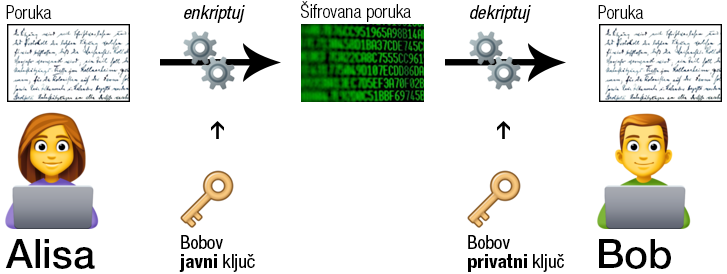
\includegraphics[width=1.0\textwidth]{material/bob_alice_enc}
    \caption{Tajna komunikacija unutar javnog kriptosistema}
    \label{fig:alice_bob_enc}
\end{figure}

\paragraph*{}
Kriptografija javnog ključa također se naziva i \textit{asimetričnom kriptografijom}, ona ne osigurava samo tajnost komunikacije kao u opisanom slučaju, nego se može koristiti i za potvrdu autentičnosti. Za takav scenario dovoljno je da Bob svojim privatnim ključem \textit{potpiše} željenu poruku ili datotetu i Alisa će biti u mogućnosti da provjeri da je ta poruka autentično kreirana od strane Boba, za tu namjenu potrebno je da Alisa posjeduje Bobov javni ključ od ranije ili da ga dobavi iz nekog povjerljivog izvora jer mora biti sigurna da neko lažno ne podmetne svoj ključ kao Bobov, više o ovoj namjeni asimetričnih kriptosistema biti će dato u zasebnom poglavlju u nastavku, no za sada je bitno imati je na umu. Spomenuti proces potpisivanja sastoji se od par kriptografskih operacija, vrlo sličnih kriptovanju poruke, no kako u ovom slučaju nije potrebno prenijeti kompletan sadržaj nego samo omogućiti verifikaciju, proces je moguće učiniti efikasnijim tako što će se poruka prije obrade privatnim ključem prethodno provući kroz neku od hash funkcija, koja će ga znatno smanjiti i ubrzati sam proces.

\subsection{Sigurnosni ciljevi}
Sigurnosni ciljevi kriptografije javnog ključa pored povjerljivosti, kao primarne funkcije, kako je već i pomenuto, uključuju i mogućnosti za provjeru integriteta i autentičnosti poruke, autentifikacija entiteta, te osiguravanje neporecivosti izvršene akcije\cite{buchmann2013introduction}, ovakav jedinstven i širok skup funkcionalnosti kriptografiji javnog ključa daje fundamentalni značaj u modernim digitalnim komunikacijama i internet poslovanju, stoga su osnovne karakteristike svakog od navedenih ciljeva ukratko opisane u nastavku.

\subsubsection*{Povjerljivost i privatnost}
Povjerljivost je osnovni sigurnosni cilj kriptografije i odnosi se na osobinu da tajni podaci neće biti dostupni neautorizovanim osobama. Povjerljivost omogućava privatnost i međusobno su usko povezane. Privatnost označava sposobnost očuvanja vlastitih podataka tajnim za sve one koji nisu eksplicitno autorizovani za njihov pregled i predstavlja osnovno ljudsko pravo garantovano članom 12 Univerzalne deklaracije o ljudskim pravima\cite{assembly1948universal}:

\begin{quote}
\textit{"Niko ne smije biti podvrgnut samovoljnom miješanju u njegovu privatnost, obitelj, dom ili dopisivanje, niti napadima na njegovu čast i ugled. Svako ima pravo na zakonsku zaštitu protiv takvog miješanja ili napada."}
\end{quote}

\paragraph*{}
Mnoštvo je primjera važnosti povjerljivosti i privatnosti u savremenoj eri opšteprisutne digitalizacije i internet poslovanja, nažalost narušavanje ovih temeljnih vrijednosti postalo je gotovo normalna i svakodnevna pojava bilo da se radi o krađi osjetljivih podataka i digitalnih dobara od strane malicioznih agenata ili prisluškivanju od strane korporativnih i vladinih agencija koje vrše masovno špijuniranje na globalnom nivout prikupljanjem privatnih podataka putem raznorodnih programa\cite{wleaks}.

\subsubsection*{Autentifikacija entiteta}
Autentifikacija se odnosi na proces utvrđivanja stvarnog identiteta, navedeni identitet može se odnositi na osobu, kompaniju ili bilo koji drugi koncept koji se od drugog razlikuje po sebi svojstvenim osobinama. Za isti proces može se približno precizno koristiti i termin identifikacija. Poznavanje identiteta u okviru digitalnog okruženje često je neophodno za ispravno funkcionisanje programskog rješenja i pravilnu raspodjelu autorizacija, kao i za relacije povjerenja između različitih kategorija korisnika. Često se za ovu namjenu koriste korisnička imena i lozinke kao najprostiji vid implementacije, no mnogo su pouzdaniji namjenski izrađeni repozitoriji identiteta u vidu specifičnih rješenja ili infrastrukture javnih ključeva (\textit{PKI - public key infrastructure}), koji omogućavaju mnogo sigurniju autentifikaciju, bolje provođenje dobrih sigurnosnih praksi, širi spektar primjene i bolju integraciju. Aplikacija izrađena u okviru ovog rada sadrži namjenski izrađen pokazni repozitorij identiteta i javnih ključeva u vidu Logit API implementacije.

\subsubsection*{Integritet i autentičnost poruke}
Integritet se odnosi na garanciju da podaci nisu mijenjani nakon što ih je izvorni autor sačinio, mnoštvo je bitnih aktivnosti gdje je upravo ovakva garancija od iznimne važnosti. Koncept integriteta dodatno se proširuje kroz pojam autentičnosti poruke, gdje se zahtjeva i mogućnost utvrđivanja njenog izvorišta, te njegova autentifikacija. Ove aktivnosti izvode se putem digitalnog potpisivanja i vjerodostojnih repozitorija koji sadrže provjerene identitete entiteta koji se autoriziraju, najčešće u vidu već opisanih PKI.

\paragraph*{}
Kao primjer možemo uzeti svakodnevno poznate korisničke scenarije, svaki računarski program ili nadogradnja kada se distribuira krajnjim korisnicima može biti naknadno izmjenjen u cilju izvršavanja određenih zlonamjernih aktivnosti koje mogu naštetiti korisniku, da bi se ovo izbjeglo većina savremenih operativnih sistema podržava određeni način provjere integriteta softvera prilikom instalacije na korisničkom računaru i autentičnost identiteta njenog izvorišta, ovakve provjere posebno su bitne u sigurnosno osjetljivim okruženjima i djalatnostima gdje bi pokretanje zlonamjernog koda moglo ugroziti živote ili uzrokovati veliku materijalnu štetu, primjeri takvih sistema su računari u zdravstvu i kontrolni sistemi javnih infrastruktura, poput aerodroma, električne ili vodovodne mreže, no nikako ne treba zanemariti i kućne korisnike koji su itekako izloženi raznim vrstama sigurnosnih prijetnji. Za namjene utvrđivanja integriteta i autentifikacije izvorišta programskih rješenja održavaju se repozitoriji sa identitetima softverskih razvojnih kuća i njihovim ključevima.

\paragraph*{}
Dodatno utvrđivanje integriteta poruke i autentifikacija učesnika se koristi u okviru aplikacije za bilježenje prisustva studenata predložene u okviru ovog rada na način da se potpisano vrijeme i lokacija svih studentskih uređaja potpisuje predavačkim ključevima unutar jedinstvene sesije (npr. nastavnog časa) koju po zaključenju nije moguće naknadno mijenjati bez narušavanja integriteta navedene sesije. Identitet svih učesnika i autentičnost njihovih potpisa provjerava se korištenjem namjenskog repozitorija na Logit API.

\subsubsection*{Neporecivost}
Neporecivost je osobina podataka koja sprječava poduzimača određene aktivnosti da istu porekne nakon njenog okončanja, npr. slanje poruke, novčana transakcija ili prisustvo predavanju. Kod primjera prisustva, radi se o nemogućnosti studenta da nakon što digitalno prijavi svoje prisustvo na predavanju unutar predložene Logit NFC aplikacije naknadno to prisustvo porekne jer postoji jedinstveni digitalno potpisan trag koji to dokazuje, za čvrst dokaz neophodno je osigurati i jaku povezanost korisnika i nosioca identiteta, u ovom slučaju mobilnog uređaja, za ovakve namjene posebno su pogodne višefaktore metode identifikacije koje uključuju i biometrijske osobine.

\section{RSA kriptosistem}
Rivest, Shamir i Adelman\cite{rivest1978method} predložili su kriptosistem koji može osigurati osobine privatnosti i potpisivanja poruka ekvivalentne ili bolje od onih kakve posjeduje papirna pošta. Njihov sistem baziran je na konceptu sistema javnog ključa kakav su ranije predložili Diffie i Hellman\cite{diffie1976new}. Sveukupna procedura sastoji se od procesa enkripcije \textit{E}, procesa dekripcije \textit{D} i poruke \textit{M}, te za takav sistem vrijedi:

\begin{enumerate}
  \item dešifrovanje kriptovane forme poruke \textit{M} daje \textit{M}, \[D(E(M)) = M\]
  \item i \textit{E} i \textit{D} su jednostavne za izračun,
  \item javno obznanjujući \textit{E} korisnik ne otkriva jednostavan način za izračun \textit{D}. Praktično ovo znači da samo on može dekriptovati poruke kriptovane pomoću \textit{E}
  \item ukoliko je poruka \textit{M} prvo dešifrovana a onda šifrovana, rezultat je \textit{M}, \[E(D(M)) = M\]
\end{enumerate}

\paragraph*{}
Enkripcijska (ili dekripcijska) procedura se sastoji od \textit{opšte metode} i \textit{enkripcijskog ključa}. Opšta metoda, pod kontrolom ključa, šifruje poruku \textit{M} i rezultira šifrovanom porukom \textit{C (en. ciphertext)}. Svako može koristiti istu opštu metodu, sigurnost date procedure počiva na sigurnosti ključa. Otkrivanje enkripcijskog algoritma tada znači i otkrivanje (\textit{javnog}) ključa.

\paragraph*{}
Kada korisnik otkrije \textit{E}, on otkriva vrlo neefikasan način izračuna \textit{D(C)} testiranjem svih mogućih poruka \textit{M} sve dok se ne nađe ona koja zadovoljava \(E(M) = C\). Ukoliko je osobina (3) zadovoljena broj takvih poruka nije praktičan za izračun.

\paragraph*{}
Funkcija \textit{E} ukoliko zadovoljava osobine (1)-(3) predstavlja tzv. \textit{"jednosmjernu funkciju sa stupicom"}, a ukoliko zadovoljava i (4) onda je \textit{"jednosmjerna permutacija sa stupicom"}. Diffie i Hellman\cite{diffie1976new} uveli su koncepte jednosmjernih funkcija sa stupicom ali nisu dali implementaciju. Ove funkcije nazivaju se jednosmjernim jer ih je jednostavno izračunati u jednom smijeru ali bi trebalo biti vrlo teško u suprotnom, dok su "sa stupicom" jer su njihovi inverzi jednostavni za izračun ukoliko je poznata određena informacija, u slučaju šifrovanja je to privatni ključ. Ovakva funkcija koja također zadovoljava i (4) mora biti permutacija: svaka poruka je ciphertekst neke druge poruke i svaki ciphertekst je dozvoljena poruka. Zadovoljenje osobine (4) neophodno je za implementaciju potpisivanja.

\subsection{Ključevi i komunikacija} \label{subs:keygen}
Da bi kreirali vlastite privatne i javne ključeve učesnici moraju svaki za sebe i nasumično odabrati dva velika prosta broja \textit{p} i \textit{q} takva da nije vjerovatno da računar može izvršiti cjelobrojnu faktorizaciju \(n = p * q\), danas se minimalno preporučuju brojevi slične veličine koji daju proizvod reda 2048 bita kao sigurni do 2030. godine\cite{kaliski2003twirl}. Proizvod \textit{n} postaje dijelom javnog ključa, dok se pojedinačni faktori moraju čuvati u tajnosti zbog njihovog korištenja u derivaciji privatnog ključa.

\paragraph*{}
Korisnici također moraju izabrati i cjelobrojnu vrijednost \textit{e} takvu da, \[1 < e < \phi(n) = (p - 1)(q - 1) \wedge \gcd(e, (p - 1)(q - 1) = 1.\] Obratite pažnju da je e uvijek neparno jer je \((p - 1)(q - 1)\) parno. Dalje korisnik računa cjelobrojnu vrijednost \textit{d}, \[1 < d < (p - 1)(q - 1) \wedge de \equiv 1\bmod(p - 1)(q - 1).\] Korisnikov javni ključ sada je par \textit{(n, e)}, dok je njegov privatni ključ \textit{d}. Broj n naziva se \textit{RSA modulus}, \textit{e} je \textit{enkripcijski eksponent}, a \textit{d - dekripcijski eksponent}\cite{buchmann2013introduction}.

\paragraph*{}
Ponovno se može poslužiti primjerom Boba i Alise opisanim ranije, sada se može reči da kada je Bob korištenjem opisane procedure generisao neophodne vrijednosti ključeva i poslao Alisi svoj javni ključ, tj. vrijednosti \textit{(n, e)}, koje će ona iskoristiti za šifrovanje proizvoljne poruke \textit{m}, što tada možemo izraziti kao \[c = m^e\bmod n.\] Kada Bob primi Alisinu šifrovanu poruku \textit{c} iskoristiti će tajnu vrijednost \textit{d} i dešifrovati poruku \[m = c^d\bmod n.\]

\subsection{Digitalni potpis}
Digitalni potpis osigurava mehanizam provjere integriteta i u kombinaciji sa adekvantnom infrastrukturom - autentičnost izvorišta poruke. Ukoliko Bob želi potpisati određeni dokument, on korištenjem svog privatnog ključa izračunava jedinstveni niz bita, koji Alisi garantuje da će korištenjem Bobovog prethodno dobavljenog javnog ključa moći verifikovati da navedeni dokument nije izmjenjen u putu do nje, kao i da je Bob originalni potpisnik dokumenta, navedena interakcija prikazana je na slici \ref{fig:alice_bob_sig}, dodatno Bob u budućnosti ne može poreči da je potpisao navedeni dokument, što osigurava još jednu vrlo bitnu funkcionalnost cjelokupnog sigurnosnog sistema. Ovakav sistem predstavlja temelj na kojem je izgrađen siguran internet i digitalna ekonomija te je duboko utkan u osnovne protokole poput TLS, SSH, PGP etc.

\begin{figure}[H]
    \centering
    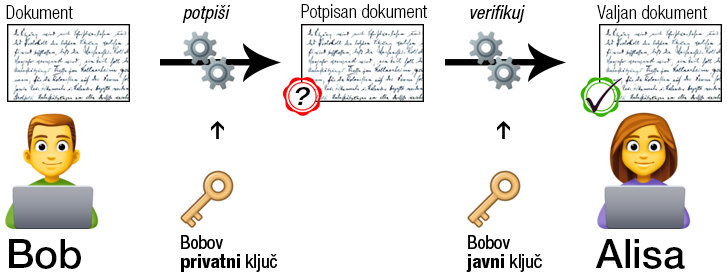
\includegraphics[width=1.0\textwidth]{material/bob_alice_sig}
    \caption{Verifikacija integriteta i autentičnosti uz garancija neporecivosti u okviru javnog kriptosistema}
    \label{fig:alice_bob_sig}
\end{figure}

\paragraph*{}
RSA šema najčešće je korišten algoritam digitalnog potpisivanja. Generacija ključeva funkcionira na istom principu kao i u primjeru šifrovanja poruke opisanom u poglavlj \ref{subs:keygen}. Svaki digitalni potpis zavisan je od poruke kao i od potpisnika, u protivnom bilo bi moguće da isti potpisnik koristi jedan potpis za više dokumenata, što ovdje nije slučaj. Da bi se uspješno implementiralo digitalno potpisivanje, kriptosistem mora zadovoljavati osobine spomenute jednosmjerne permutacije sa stupicom, budući da će dekripcijski algoritam biti primjenjivan na izvorni - nešifrovan dokument.

\paragraph*{}
Opisani primjer razmjene potpisanog dokumenta ili poruke \textit{M} između Alise i Boba može se unutar RSA kriptosistema preciznije prikazati kao: \[S = D_{B}(M),\] gdje je \textit{S} digitalno potpisana poruka a \(D_{B}\) Bobova funkcija za dešifrovanje korištenjem privatnog ključa. Kako je već napomenuto primjena funkcije za dešifrovanje na nešifrovanu poruku ima smisla u slučaju da kriptosistem zadovoljava potrebne uvjete. Ukoliko je dodatno potrebno osigurati i tajnost potpisane poruke Bob je može naknadno šifrirati Alisivnim javnim ključem, u tom slučaju Alisa po prijemu prvo vrši dešifrovanje svojim privatnim ključem da bi dobila Bobovu izvornu potpisanu poruku \textit{S}, korištenjem Bobovog javnog ključa Alisa sada "šifruje" potpisanu poruku \[M = E_{B}(S)\] time dolazeći u posjed uređenog para \textit{(M, S)} sa osobinama sličnim onima koje ima originalni fizički potpisan dokument.

\paragraph*{}
Sama praktična implementacija potpisivanja razlikuje se međutim od opisane procedure u tome da se u praksi ne vrši potpisivanje cjelokupne izvorn poruke, nego se nad njom prvobitno korištenjem hash funkcije otporne na kolizije izračunava jedinstvena hash vrijednost, pa Bob tako umjesto poruke potpisuje dobijenu hash vrijednost svojim privatnim ključem, dok na drugom kraju Alisa ponavlja proces izračunavanja hash vrijednosti koristeći Bobovu izvornu poruku, njegov javni ključ i istu hash funkciju, te dobijeni hash poredi sa Bobovim hashom, u slučaju poklapanja vrijednosti Alisa može biti sigurna u valjanost digitalnog potpisa. Jedina funkcionalna razlika ovakvog pristupa je da se koncept poruke ili dokumenta, odvaja od samog digitalnog potpisa, što olakšava rad i osigurava dodatne sigurnosne i upotrebne prednosti.

\paragraph*{}
Praktična implementacija može se formalno opisati kao primjena hash funkcije \textit{h} tako da potpis \textit{s} niza karaktera poruke \(m \in \lbrace 0,1\rbrace ^n\) glasi \[s = h(m)^d\bmod n.\] \textit{d} je u prikazanom slučaju Bobov \textit{dekripcijski eksponent}. Da bi Alisa verifikovala zaprimljeni potpis \textit{s} koristi Bobov javni ključ \textit{(n, e)} i izračunavanjem hash vrijednost \textit{h(m)} poruke \textit{m} i vrši provjeru \[h(m) = s^e\bmod n.\] Potpis je valjan ako i samo ako važi data jednakost. Za potrebe Logit sistema korištena je SHA-256 hash funkcija u kombinaciji sa RSA potpisom.

\pagebreak[4]

\section{PKI - infrastruktura javnog ključa}
Iako kriptografija javnog ključa ne zahtjeva razmjenu tajnih ključeva da bi se ostvarila povjerljiva komunikacij, vrlo je bitan aspek upravljanja ključevima, kako javnim tako i privatnim. Namjena infrastrukture javnog ključa \textit{en. PKI - private key infrastructure} je upravo to, efikasno i sigurno upravljanje javnim i privatnim ključevima tokom njihovog životnog ciklusa.

\subsection{Životni ciklus ključeva}
Životni ciklus počinje od samog generisanja, koje je opisano u poglavlju \ref{subs:keygen}, nakon čega slijedi upotrebni vijek tokom kojeg se privatni ključevi koriste za potpisivanje ili dešifrovanje primljenih poruka. Korisnici također imaju pristup javnim ključevima drugih korisnika, te ključeve koriste za šifrovanje ili verifikaciju potpisanih dokumenata. U završnoj fazi ključevi izlaze iz upotrebe bilo kroz proces zastarjevanja ili neki drugi događaj. Svaki od navedenih faza u životnom ciklusu para ključeva mora imati određene procedure da bi se osiguralo provođenje dobrih praksi u njihovom upravljanju.

\subsubsection{Generisanje i pohrana}
Prvi korak je osiguravanje pouzdanog okruženja za generisanje sigurnog para ključeva, najbolje je da tu aktivnost izvode sami korisnici, jer u tom slučaju privatni ključ ne bi trebao biti dostupan nijednoj trećoj strani, no to često nije slučaj, budući da korisničko okruženje može biti kompromitovano ili na neki drugi način neadekvatno za tu namjenu, stoga se mora pribjeći generisanju ključeva u okruženju neke povjerljive treće strane za koju se može biti sigurno da ključeve neće zloupotrijebiti. Pored navedenog i samo skladištenje ključeva, pogotovo privatnih, pruža mnoge sigurnosne izazove. Uzimajući u obzir nabrojano jasno je da navedenim problemima treba pristupiti planski i krajnje ozbiljno jer u protivnom sigurnost kompletnog sistema može biti kompromitovana od samog početka. Logit aplikacija privatne ključeve pohranjuje isključivo unutar Android repozitorija ključeva na korisničkom uređaju, za koji postoje garancije da nije moguće ostvariti pristup korištenjem bilo koje druge aplikacije.

\subsubsection{Upotrebni vijek}
Tokom upotrebne faze životnog vijeka osnovna funkcionalnost je obezbjediti siguran pristup korisničkim javnim ključevima. Pored toga da bi se mogle pružiti adekvatne garancije autentifikacije i potvrde autentičnosti neophodno je utvrditi i provesti jasne procedure koje će osigurati jasnu povezanost entiteta/osoba sa ključevima, u protivnom može doći do krađe identiteta i lažnog predstavljanja. Logit API vršit funkciju repozitorija javnih ključeva za korisnike sistema i povezuje korisnike sa njihovim ključevima, osigurana je osnovna provjera identiteta putem korisničke prijave na fakultetski ZAMGER sistem.

\subsubsection{Kraj životnog ciklusa}
Dodatno potrebno je utvrditi jasne procedure za kraj životnog vijeka i pohranu starih ključeva, kod Logit API repozitorija ne postoji vremenski ograničen vijek trajanja para ključeva, no pri svakoj novoj instalaciji aplikacije ili zamjeni uređaja, stari par ključeva se arhivira a novogenerisani ključevi se koriste kao sigurnosno relevantni. Pored navedenih funkcionalnosti Logit API se koristi i kao repozitorij potpisanih dokumenata, u ovom slučaju, prisutava predavanjima, no to izlazi iz okvira domena PKI i može se smatrati dodatno funkcionalnošću.

\subsection{Hijerarhija povjerenja}
Za praktičnu upotrebu kriptografije javnog ključa neophodno je da korisnici vjeruju u autentičnost dostupnih javnih ključeva. Stoga su pored prostog direktnog modela povjerenja sa dva učesnika koji razmjenjuju sopstvene javne ključeve uspostavljene raznovrsne hijerarhije povjerljivih učesnika koje omogućavaju formiranje složene mreže koja i sama kao svoju osnovu koristi digitalni potpis i dostupne kriptografske metode.

\begin{figure}[H]
    \centering
    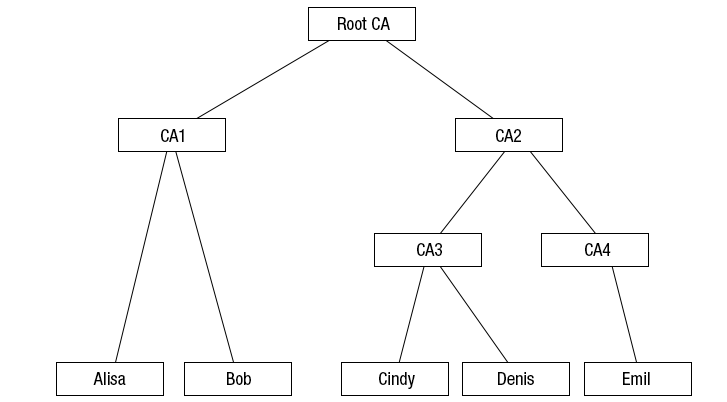
\includegraphics[width=1.0\textwidth]{material/pki}
    \caption{Primjer hijerarhijske infrastrukture javnog ključa}
    \label{fig:pki}
\end{figure}

\paragraph*{}
Primjer jedne složene hijerarhije povjerenja prikazan je na slici \ref{fig:pki}, u ovakvom modelu javne ključeve svih nižih učesnika potvrđuje CA \textit{(en. certification authority)}, koji ujedno na adekvatan način vrši i verifikaciju autentičnosti. Većina ovakvih hijerarhijskih PKI arhitektura uređena je u skladu sa standardom X.509. U ovakvom okruženju može da učestvuje više nivoa posrednih CA \textit{(en. intermediate CA)} i obično je uređeno u strukturu drveta sa listovima, gdje se u korjenu nalazi CA \textit{(en. root CA)} kojeg svi posredni CA uzimaju kao pouzdanog i koji sam potpisuje svoj certifikat. Na dnu strukture drveta nalaze se krajnji korisnici kriptosistema. Da bi se ostvarila relacija povjerenja između dva korisnika, nije neophodno da oni dijele isti posredni CA, dovoljan uslov je da se može napraviti veza prema jednom CA u kojeg oba korisnika imaju povjerenje da bi pomenuta relacija bila zadovoljena.

\paragraph*{}
Primjer jedne relacije povjerenja iz priložene hijerarhije može se formirati između korisnika Alisa i Emil, gdje se da jasno utvrditi \textit{certifikacijska putanja} koja za oba korisnika seže do korjenskog Root CA, ilustrativno za Alisu i Emila važi: \[Alisa \to CA1 \to Root CA\] \[Emil \to CA4 \to CA2 \to Root CA\] dubina certifikacijske putanje također može da igra ulogu u zavisnosti od različitih zahtjeva, u nekim slučajevima duže putanje, poput Emilove se mogu smatrati nepouzdanim za određene namjene, u svakom slučaju poželjno je korištenje što bližih međusovnih putanja.

\paragraph*{}
Logit API posjeduje svoj set ključeva kojim potpisuje sve zaprimljene korisničke sesije prisustva. Da bi se upotpunio model povjerenja neophodno je da se LAPI ceritikat potvrdi od strane institucije koja implementira navedeni sistem, u ovom slučaju Elektrotehničkog fakulteta, koja je dalja poveznica na vanjski korjenski CA i omogućava izgradnju šireg sistema povjerenja gdje više institucija koje koriste isti sistem može ostvariti posredne relacije povjerenja. Važno je istaknuti također da korisnici registracijom bivaju uključeni u LAPI repozitorij, što se može smatrati ekvivalentom certifikata, dodatno korisnici međusobno potvrđuju prisustvo a samim tim ostvaruju vezu međusobnog povjerenja, jer aktivnost prikupljanja potpisa inherentno utvrđuje međusobnu identifikaciju korisnika. Prikaz takvog modela dat je na slici \ref{fig:logit_pki}.

\begin{figure}[H]
    \centering
    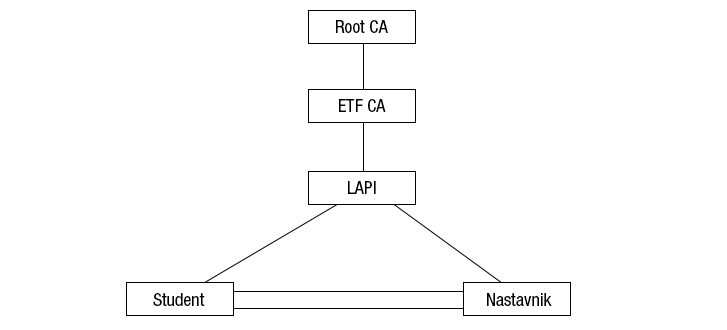
\includegraphics[width=1.0\textwidth]{material/logit_pki}
    \caption{Prikaz Logit PKI hijerarhije}
    \label{fig:logit_pki}
\end{figure}

\subsection{Certifikati}
Bitan aspekt PKI je obezbjeđivanje potvrde autentičnosti za javne ključeve, jedan od načina da se to ostvari su svakako certifikati, tj. strukture koje povezuju javne ključeve sa entitetima ili osobama, najčešće su pohranjeni na PKI koji se brinu da osiguravaju što jaču garanciju relacije između entiteta i javnog ključa. U cilju iskoristivosti neophodno je da certifikati obezbjede određeni nivo tehničkih i domenski relevantnih podataka, u većini slučajeva to su:

\begin{itemize}
    \item ime ili naziv entiteta za čiji javni ključ je vezan
    \item javni ključ entiteta
    \item korišteni kriptografski algoritam
    \item serijski broj
    \item period važenja
    \item naziv izdavača certifikata, koji je ujedno i potpisnik
    \item namjena i ograničenja korištenja javnog ključa
\end{itemize}

\paragraph*{}
Sam sadržaj certifikata u većini slučajeva je standardiziran, danas najčešće standardom X.509, gdje se i izdati certifikat naziva prema standardu X.509 certifikat, primjer jednog takvog certifikata dat je na slici \ref{img:etf_cert_gen}, navedene su osnovne informacije o certifikatu i opšte informacije pobrojane iznad, dodatno na slici \ref{img:etf_cert_tree} prikazana je certifikacijska putanja datog certifikata. Pored navedenih informacija certifikat obično sadrži mnoštvo i drugih informacija, budući da standard dopušta proširivanje da bi obuhvatio širok domen primjene. Bitno je još napomenuti da zbog vrlo široke primjene u različitim programskim rješenjima postoji mnoštvo različitih formata zapisivanja i razmjene samih certifikata, te je često neophodno konvertovati certifikate u jedan od odgovarajućih formata.

\paragraph*{}
X.509 certifikati koriste ASN.1 \textit{(en. abstract syntax notation version 1)} kao jezik za izvornu specifikaciju osobina certifikata, pomoću navedenog jezika moguće je izraziti mnoštvo kompleksnih struktura za opis osobina certifikata, jedan od mnoštva načina da se navedena specifikacija zapiše je DER \textit{(en. distinguished encoding rules)}, koja je dalje bazirana na BER pravilima za zapisivanje \textit{(en. basic encoding rules)}, navedene strukture predstavljaju svojevrsnu hijerarhiju deskriptivnih jezika i meta-jezika sličnu relaciji SGML, HTML.

\begin{figure}[H]
    \centering
    \begin{subfigure}{.5\textwidth}
        \centering
        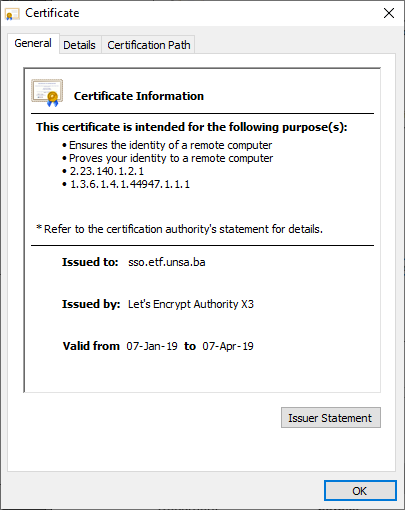
\includegraphics[width=1\textwidth]{material/etf_cert_gen}
        \caption{opšte karakteristike}
        \label{img:etf_cert_gen}
    \end{subfigure}%
    \begin{subfigure}{.5\textwidth}
        \centering
        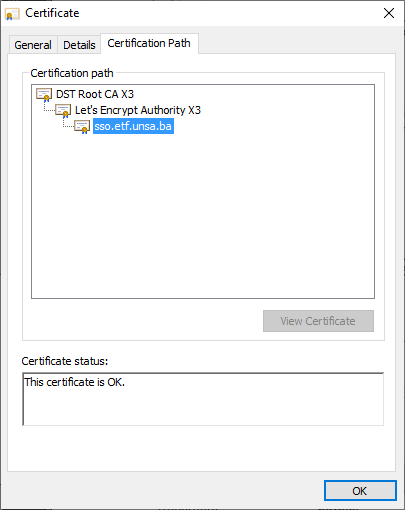
\includegraphics[width=1\textwidth]{material/etf_cert_tree}
        \caption{lanac povjerenja}
        \label{img:etf_cert_tree}
    \end{subfigure}
    \caption{Osobine certifikata}%
    \label{img:etf_cert}
\end{figure}

\paragraph*{}
Logit aplikacija interno koristi namjenski i nestandardni format certifikata, no sve LAPI i korisničke certifikate moguće je pretvoriti u bilo koji od standardnih formata i tako ostvariti interakciju sa ostalim sistemima ukoliko se za to ukaže potreba. Dovoljno je na Logit API strani implementirati novu URI lokaciju koja bi vraćala certifikate u standardizovanom formatu.
	\chapter{Prijedlog rješenja}
U skladu sa datim zahtjevima predložena je izrada aplikacijske platforme pod nazivom Logit (
\gls{LAPP}), opisane u nastavku, sa detaljnim tehničkim detaljima u narednim poglavljima. Uzimajući u obzir data ograničenja, te funkcionalne i nefunkcionalne zahtjeve određeno je da se korisnička aplikacija izradi na Android platformi sa podrškom za Android API nivo počevši od nivoa 19 (4.4 KitKat), to je najniži nivo koji omogućava korištenja naprednih NFC i kriptografskih funkcionalnosti te osigurava dobru pokrivenost potencijalne korisničke baze sa ukupnom adopcijom od preko 90\% za navedenu ili višu verziju\cite{droidstats}. Za uspješan rad aplikacije neophodno je da korisnički uređaj podržava i NFC funkcionalnosti, prema prognozama analitičke kuće IHS Technology, do 2020. godine svaki treći uređaj imati će podršku za NFC.\cite{nfcforecast}

\section{Logički model rješenja}
Priloženi dijagrami interakcije osnovnih funkcionalnosti Logit platforme i pripadajući opis imaju za cilj stvoriti opštu sliku sistema, te tako olakšati praćenje tehničkog modela rješenja datog u nastavku. Tehnički model opisuje dosta detaljniju sliku funkcioniranja sistema i može služiti kao svojevrstan uvod u kod platforme.

\subsection*{Registracija korisnika}
\begin{figure}[H]
    \centering
    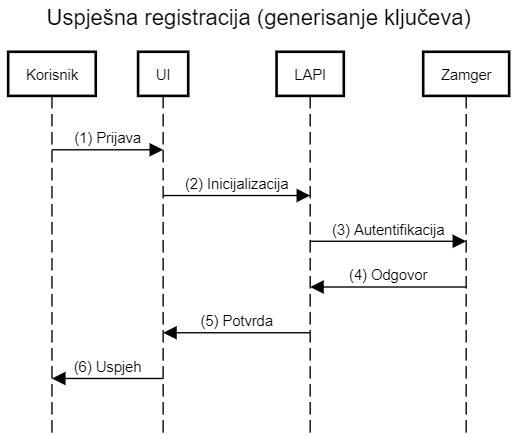
\includegraphics[width=0.7\textwidth]{material/dia/01_registracija}
    \caption{Dijagram interakcije - uspješna registracija i generisanje ključeva}
\end{figure}
\paragraph*{}
Nakon uspješne instalacije aplikacije na korisnički Android uređaj (DEVICE) potrebno je obaviti proces registracije koji se izvršava u dva bitna koraka. Prvi korak sastoji se od unosa već postojećih autentifikacijskih podataka za ZAMGER sistem Elektrotehničkog fakulteta, korisnik se korištenjem datih podataka posredstvom LAPI servisa autentificira na ZAMGER sistemu, bitno je napomenuti da Logit platforma ne sprema korisničku lozinku ZAMGER sistema, navedeni podaci se koriste isključivo za povezivanje postojećeg identiteta i novogenerisanog para korisničkih RSA ključeva (KEYS), što je ujedno i drugi korak u procesu registracije na Logit platformu.

\paragraph*{}
U slučaju uspješnje autentifikacije, korisnika se obavještava o završenoj registraciji te se preusmjerava na glavni ekran za bilježenje prisustva. Generisani javni ključ (CERT) i identifikacioni podaci korisnika spremaju se u LAPI direktorij korisničkih certifikata.

\subsection*{Bilježenje prisustva studenta}
Bilježenje prisustva studenata od strane predmetnog nastavnika izvodi se u Master (M) modu funkcionisanja aplikacije, aplikacija se pri samom pokretanju i nakon uspješno obavljene registracija automatski stavlja u takav mod operacije i u njemu ostaje sve dok je upaljen ekran korisničkog uređaja (DEVICE) i Logit aplikacija (UI) se izvršava u prednjem planu \textit{(en. foreground)}, navedene zahtjeve diktira sama Android platforma.

\begin{figure}[H]
    \centering
    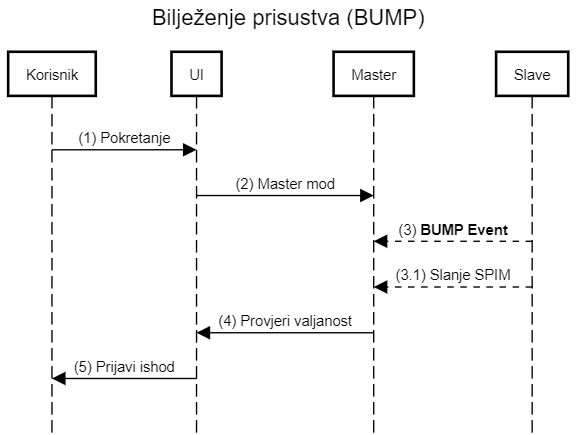
\includegraphics[width=0.7\textwidth]{material/dia/02_bump}
    \caption{Dijagram interakcije - bilježenje prisustva studenata (Master BUMP)}
\end{figure}
\paragraph*{}
Ukoliko su ispunjeni prethodno pobrojani zahtjevi, dovoljno je da student sa podešenom Logit aplikacijom na svom uređaju prinese slave (S) uređaj master (M) uređaju i da njegovo prisustvo bude zabilježeno i prikazano na ekranu M uređaja. Samu interakciju (BUMP) inicira studentski S uređaj. Prilikom ovog BUMP događaja dolazi do razmjene kriptografski potpisanih podataka o vremenu i lokaciji (SPIM) sa S na M, gdje M vrši validaciju primljenih podataka poredeći studentsko vrijeme i lokaciju sa vremenom i lokacijom na M uređaju, gdje se prisustvo odbija ukoliko se ustanovi pokušaj lažiranja podataka.

\subsection*{Prijava prisustva}
\begin{figure}[H]
    \centering
    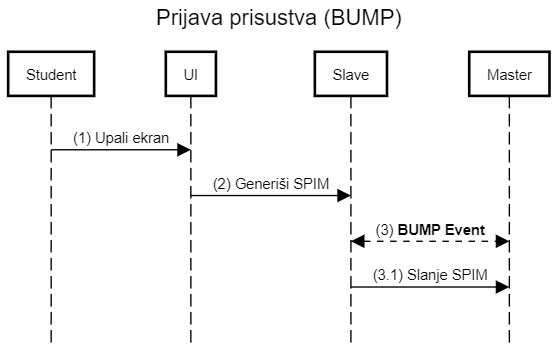
\includegraphics[width=0.7\textwidth]{material/dia/03_prijava}
    \caption{Dijagram interakcije - prijava prisustva studenta (Slave BUMP)}
\end{figure}

\paragraph*{}
Studentski S uređaj i M uređaj nastavnog osoblja podešavaju se na isti način opisan iznad, jedina praktična razlika javlja se prilikom korištenja, gdje je za S uređaj čije se prisustvo bilježi dovoljno upaliti ekran uređaja da bi se mogla ostvariti BUMP interakcija prislanjanjem S na M. Ovo je moguće jer se NFC HCE emulator Logit aplikacije izvršava u pozadini Android sistema.

\subsection*{Pohranjivanje potpisa sesije na LAPI}
Svako bilježenje prisustva unutar Logit Android UI odvija se unutar sesije (SESS) koja se automatski započinje prilikom prvog uspješno zabilježenog prisustva i traje sve dok korisnik ne izvrši pohranu navedene sesije na LAPI servis. Klikom na SYNC dugme prikupljeni podaci šalju se LAPI servisu, provjeravaju se jedinstveni potpisi studenata te potpis ukupne sesije od strane M uređaja, ukoliko se ne pronađu nepravilnosti navedeni podaci se pohranjuju u LAPI repozitorij potpisa, takvi podaci kriptografski su osigurani od naknadne izmjene.

\begin{figure}[H]
    \centering
    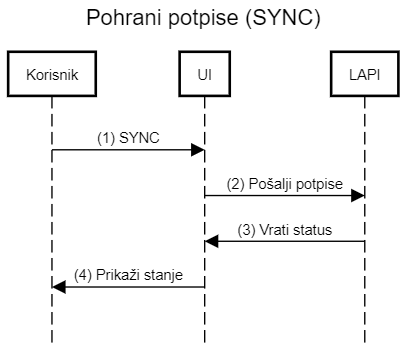
\includegraphics[width=0.6\textwidth]{material/dia/04_sync}
    \caption{Dijagram interakcije - pohranjivanje potpisa na LAPI (SYNC)}
\end{figure}
\paragraph*{}
Potpisi pohranjeni u LAPI repozitoriju mogu dalje biti korišteni u integrisanim aplikacijskim rješenjima koja zahtijevaju ovakvu vrstu podataka pomoću ponuđenog LAPI REST interfejsa, te se mogu smatrati relevantnim i sigurnim dokazom prisustva.

\section{Tehnički model rješenja}
Uvodi se dodatno pojam lokacijskog dokaza\cite{locproof} koji u širem smislu u kontekstu podređenog korisnika (en. slave), obuhvata kriptografski potpisan korisnički identitet, korisnički uređaj, vrijeme i GPS lokacijske podatke korisničkog uređaja. Za svrhu osiguranja jedinstvenosti identiteta i vjerodostojnosti potvrde lokacijskih dokaza odabrano je korištenje RSA asimetrične enkripcije, gdje se pri uspješnoj autentifikaciji generiše jedinstveni set ključeva za korisnički uređaj, privatnom dijelu ključa nije moguće pristupiti izvan aplikacije (SEC1), niti je moguće eksportovati ključ (SEC2), a u određenom vremenskom period može postojati samo jedan valjan set ključeva za jednog korisnika jer se raniji ključevi ne uzimaju u obzir ukoliko postoji noviji set (SEC3), sprječavajući tako replikaciju identiteta na više uređaja.

\paragraph*{}
Pored Android komponente aplikacije (UI) izrađena je i serverska aplikacija u programskom jeziku Python (LAPI), čija je namjena posredovanje u komunikaciji sa autentifikacijskim agentom (ZAMGER), te pohranjivanja i održavanje javnih korisničkih kriptografskih ključeva (CERT) i njihovo povezivanje sa autentifikacijskim podacima korisnika, pored toga služi i kao repozitorij za potpisana prisustva (ATTN). Na ovu komponentu se može gledati kao na integrisani namjenski repozitorij korisničkih certifikata i domenski repozitorij neporecivih i neizmjenjivih lokacijskih dokaza (SPIM).

\paragraph*{}
Budući da na Elektrotehničkom fakultetu u Sarajevu postoji SSO (en. Single-Sign On) politika autentifikacije, u serverskoj komponenti (LAPI) je implementiran autentifikacijski posrednik koji prilikom prvog pokretanja aplikacije prijavljuje korisnika koristeći postojeće pristupne podatke, tom prilikom u slučaju uspješne prijave generiše se i jedinstveni set RSA ključeva dužine 2048 bita (KEYS), koji se pohranjuju na korisničkom uređaju (DEVICE), a javni dio, tj. certifikat (CERT) se pohranjuje i u repozitorij ključeva (LAPI) sa poveznicom na korisnički identitet, kasnije se ti certifikati koriste za provjeru valjanosti potpisa lokacijskih dokaza (SPIM).

\paragraph*{}
Da bi se osigurala jednostavnost korištenja aplikacije odabrana je implementacija HCE emulacijskog načina rada NFC komunikatora koji omogućava korisniku da izvrši komunikaciju sa drugim uređajem bez potrebe da pokreće aplikacijski prozor na svom uređaju, dovoljno je da upali ekran svoj uređaja i prinese ga master (M) uređaju koji prikuplja potpise, u ovom slučaju drugoj instanci Logit aplikacije na kojoj je pokrenuta aktivnost za prikupljanje potpisa (LAPP).

\paragraph*{}
Približavanjem mobilnih uređaja (BUMP) otvara se jednosmjerni komunikacijski kanal u smijeru od slave (S) prema master (M) uređaju korištenjem ISO/IEC 14443 Tip A komunikacijskog protokola pri čemu se emulira NFC Forum Tag tipa 4 i putem NDEF Aplikacije prenosi jedna NDEF poruka (NDEFMSG) koja sadrži vremensko-lokacijski dokaz potpisan od strane korisnika, nadalje u tekstu označen kao SPIM (en. spime)\cite{bruces}.

\paragraph*{}
Po primitku poruke nadređeni uređaj (en. master) koji osluškuje da mu se pridruže podređeni uređaji (en. slave) i ima pokrenutu Logit aplikaciju, tu poruku sprema u lokalni repozitorij potpisa ukoliko ona zadovolja uslove da očitana slave GPS lokacija nije udaljena više od 50 metara od očitane master GPS lokacije (VK1 - validacijski kriterij \#1), te da podešena razlika satova master i slave uređaja nije veća od 300 sekundi (VK2), bez da nad SPIM objektom vrši ikakve izmjene, ukoliko SPIM objekat ne zadovoljava date validacijske kriterije odbija se i ispisuje se odgovarajuća poruka na master ekranu. Moguće je naknadno klikom na validacijsko dugme (ACTVAL) u korisničkom interfejsu izvršiti provjeru svih prikupljenih potpisa tokom jedne sesije (SESS), tom prilikom se, ukoliko postoji mrežna veza; svi potpisi pošalju Logit serveru (LAPI) na provjeru i vraća se stanje valjanosti potpisa za sve proslijeđene SPIM objekte.

\paragraph*{}
Ukoliko master (M) želi da pohrani SPIM objekte iz jedne sesije (SESS) na Logit server (LAPI), klikom na sinhronizacijsko dugme u interfejsu (ACTSYNC), on vrši dodatno potpisivanje svakog SPIM objekta svojom komponentom privatnog ključa (MPRK), tako što potpiše hash (SHA256) vrijednost SPIM objekta (AID) sa dodatim svojim jedinstvenim master korisničkim imenom (MUSER) i jedinstvenim identifikatorom sesije (SID) i dodatno generiše SHA256 vrijednosti tih potvrda (CID), nakon čega objedinjuje sve CID vrijednosti i dodatno ih potpisuje svojim MPRK, sve te vrijednosti šalje Logit server (LAPI) na pohranjivanje, ovakvom procedurom se obezbjeđuje neporecivost i neizmjenjivost SPIM i SESS objekata, jer onemogućava izmjene pojedinačnih SPIM objekata, te brisanje ili dodavanje objekata u finaliziranoj sesiju (SESS) od strane malicioznih aktera bez da naruši integritet SHA256 vrijednosti.

\paragraph*{}
Uzmimajući u obzir bitnost rješenja i visoku vjerovatnoću svakodnevne primjene kod ciljane korisničke grupe, te izazove koje takav slučaj korištenja predstvalja omogućena je i direktna e-mail komunikacija za prijavu grešaka ili slanje prijedloga sa glavnog korisničkog interfejsa (ACTBUG). Kako se radi o slojevitom i kompleksnom softverskom rješenju za više detalja referirati se na izvorni kod priložen u dodatku.

\begin{figure}[H]
    \centering
    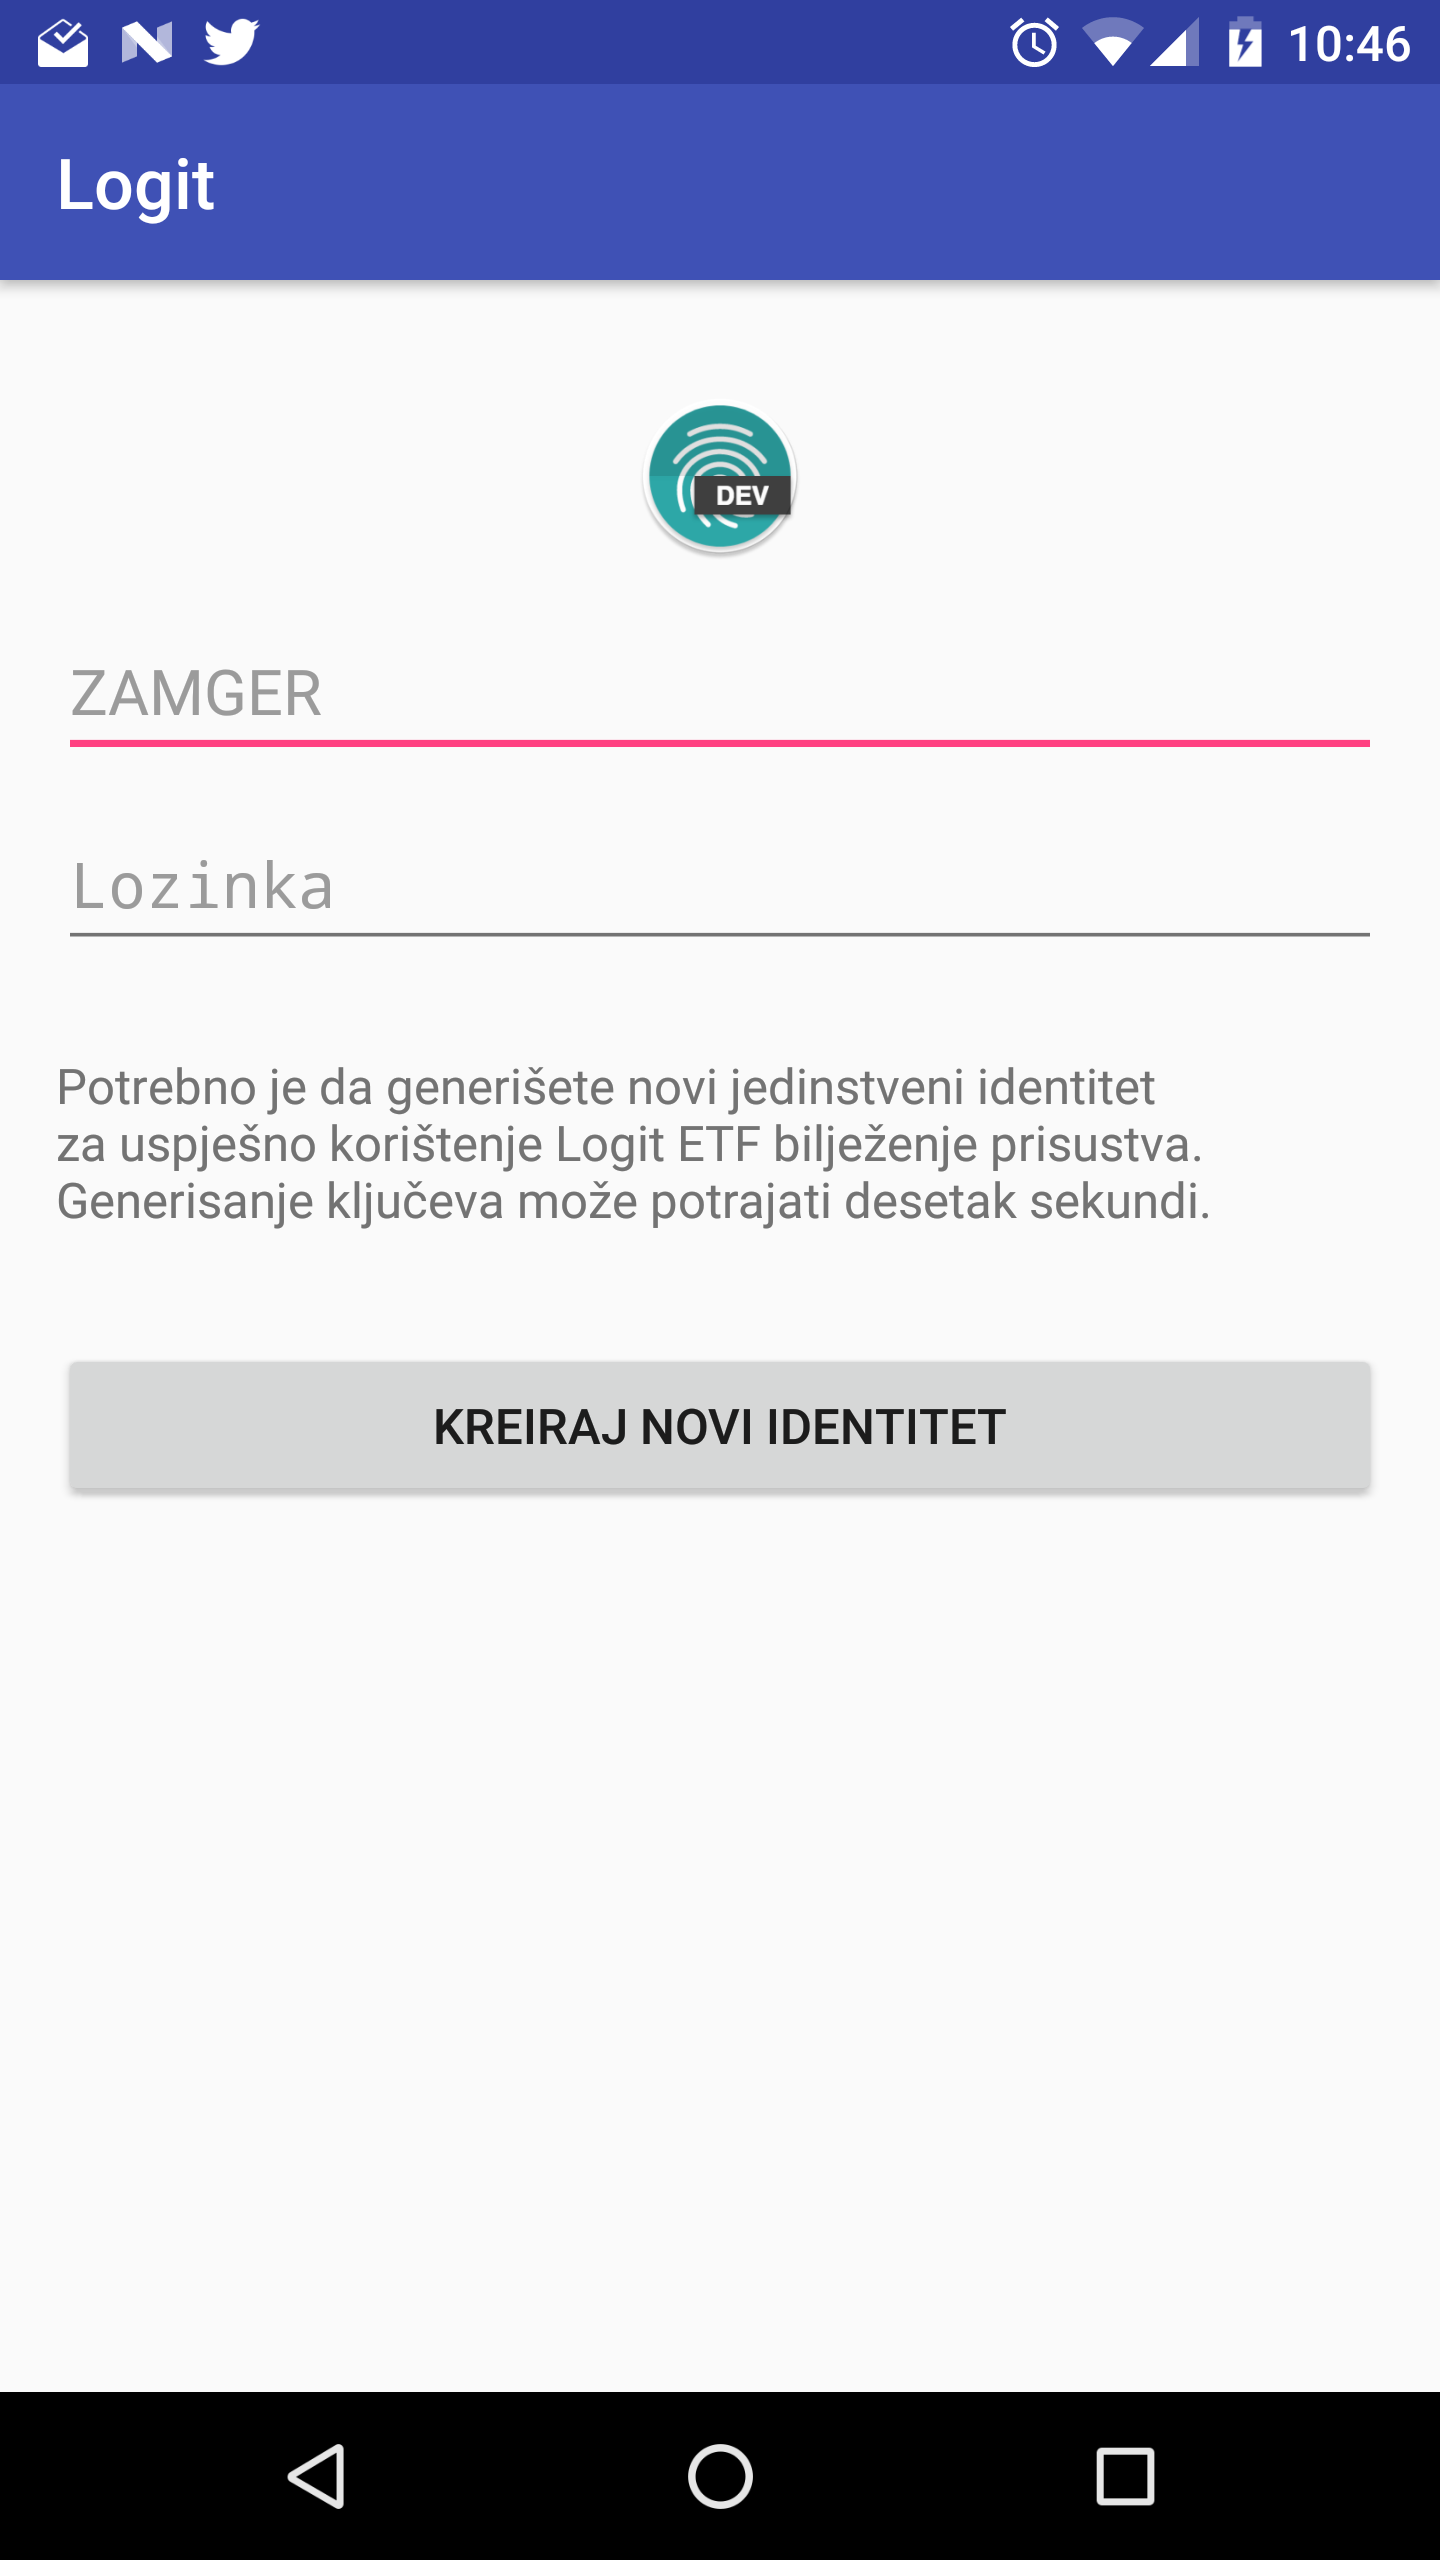
\includegraphics[width=0.45\textwidth]{material/00-login}
    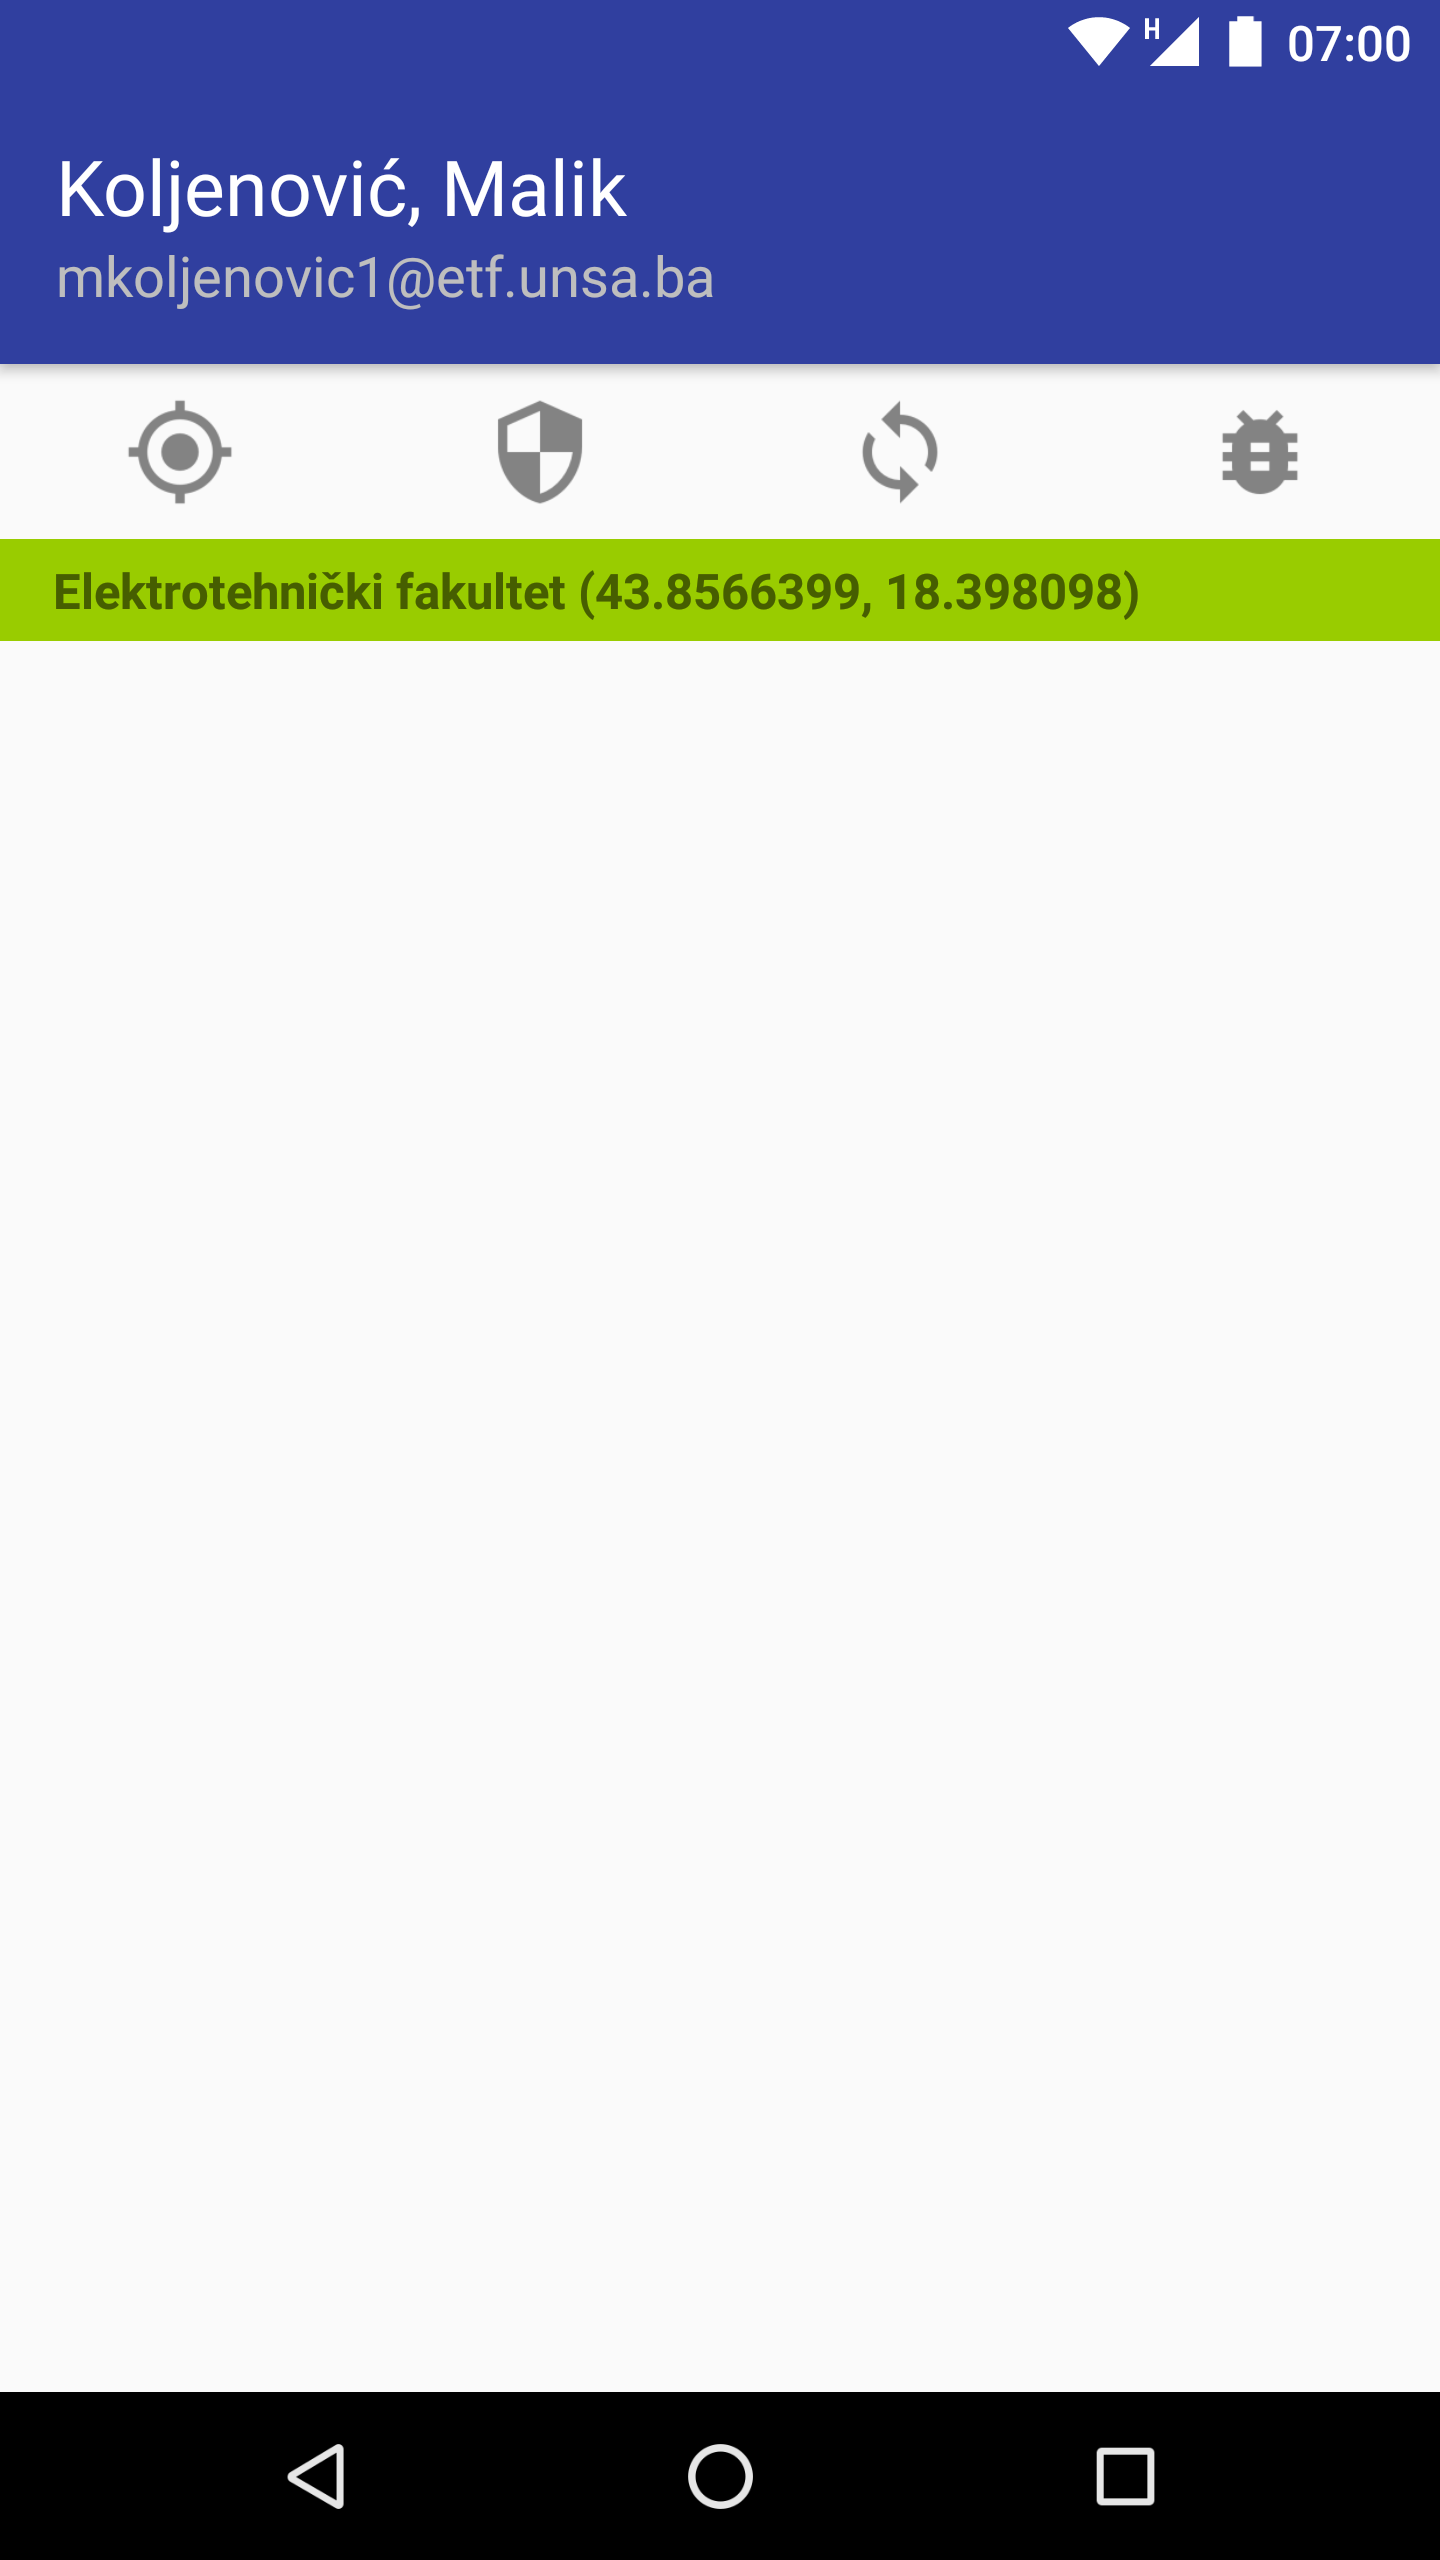
\includegraphics[width=0.45\textwidth]{material/01-attendance}
    \caption{Logit UI Android prikaz korisničkog interfejsa}
\end{figure}
	\chapter{Pregled korištenih tehnologija} \label{chapter:tech}

\section{NFC \textit{(en. near-field communication)}}
NFC skup protokola omogućava uspostavu komunikacijskog kanala između dva uređaja koji se nalaze u neposrednoj blizini jedan drugog (1-4 cm) i razmjenu podataka između njih\cite{NFCProtocol}. Komunikacija se odvija na način da MASTER uređaj osluškuje signal na prijemniku i u slučaju detektovanje SLAVE signala uređaja pošiljaoca, propisanog istim standardom zaprima podatke i vrši obradu nad njima, komunikacija se u većini slučajeva odvija jednosmjerno kratkim standardiziranim porukama (NDEF), no moguće je ostvariti i half-duplex komunikaciju između uređaja, kao i razmjenu nestandardnih poruka, u kojem slučaju se sam korisnik mora pobrinuti za implementaciju kompletnog komunikacijskog protokola. Potpuni detalji implementacija dati su u referencama relevantnih standarda u nastavku tehničkog pregleda, odličnu sintezu detalja i implementacije daju Igoe, Coleman i Jepson\cite{Igoe2014}.
\subsection{NXP NTAG216}
U cilju zadovoljenja postavljenih funkcionalnih zahtjeva bilo je neophodno odabrati NFC Tag platformu koja će odrediti relevantne standarde pohrane binarnih podataka na uređajima kao i pripadajuće komunikacijske protokole, također dodatno su postavljeni zahtjevi ekonomičnosti implementacije i kompatibilnosti sa postojećim čitačima. Uzimajući u obzir nabrojane kriterije odabrana je platforma NTAG216 proizvođača NXP Semiconductors\cite{NTAG216} bazirana na NFC Forum Tag tipu 2 i ISO/IEC14443 Tip A specifikaciji\cite{NFCTag2}\cite{ISO14443}. 

\paragraph*{}
Mogućnosti navedene platforme dostatne su za ispunjenje navedenih funkcionalnih uslova, a pružaju i neke dodatne sigurnosne mehanizme - poput neizmjenjivog jedinstvenog serijskog broja svakog taga (Tag UID) potpisanog kriptografskim ključem proizvođača, navedena funkcionalnost nije implementirana u predstavljenom rješenju jer se bazira na zaštićenoj NXP tehnologiji i nije kompatibilna sa HCE emulacijom, no umnogome može doprinijeti ukupnoj sigurnosti fizičkih Tag čipova u slučaju produkcijske implementacije rješenja. U nastavku je data proizvođačka lista izdvojenih funkcionalnosti NTAG216:

\begin{itemize}[noitemsep]
    \item 7-bajtni UID programiran od strane proizvođača za svaki tag
    \item mogućnost jednokratnog programiranja i zaključavanja taga za dalje izmjene
    \item mogućnost read-only zaključavanja taga
    \item potpis originalnosti baziran na kriptografiji eliptičnih krivih
    \item zaštita memorijskih operacija 32-bitnom lozinkom
\end{itemize}

\paragraph*{}
Proces emulacije taga svodi se na što vjerniju reprezentaciju memorijskog prostora fizičkog uređaja u skadu sa relevantnim standardima, a opcionalno i dodatnih nestandardnih funkcionalnosti u vidu komunikacijskog protokola za korištenje naprednih funkcionalnosti date platforme. Kao minimum neophodan za standardnu komunikaciju NDEF porukama potrebno je emulirati generičko zaglavlje u obliku \textit{CC - capability container} i potpun zapis same NDEF poruke unutar korisničkog memorijskog prostora, potpun prikaz organizacije memorije NTAG216 platforme dat je na slici \ref{fig:ntag_mem}\cite{NTAG216}. Za emulaciju nestandardnih dijelova, poput zaštite čitanja korisničkog memorijskog prostora lozinkom ili emulaciju serijskog broja, za svaku različitu platformu neophodno je implementirati komunikacijski protokol u skladu sa proizvođačkom specifikacijom.

\begin{figure}[H]
    \centering
    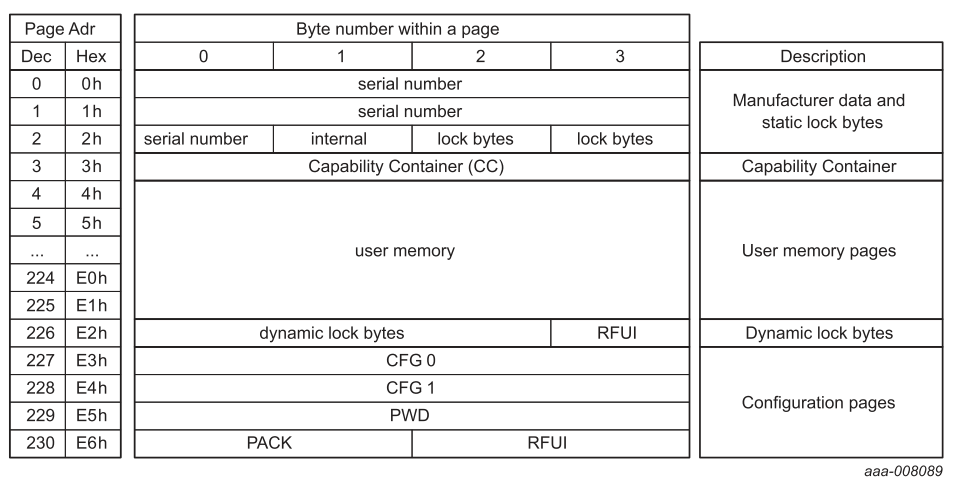
\includegraphics[width=1\textwidth]{material/ntag216-memory}
    \caption{NTAG216 organizacija memorije}
    \label{fig:ntag_mem}
\end{figure}

\subsection{NDEF \textit{(en. NFC Data Exchange Format)}}
NDEF specifikacija definiše \textbf{format enkapsulacije poruke} za razmjenu informacija između dva NFC uređaja. NDEF je lagan binarni format poruke i može se koristiti za enkapsulaciju jednog ili više aplikacijski-definisanih tereta \textit{(en. payload)} raznih vrsta i veličina unutar jedne NDEF poruke. Svaki teret opisan je od strane tipa, dužine i opcionalnog identifikatora. Identifikatori tipa mogu biti URI, MIME media tipovi, ili NFC-specifični tipovi. NDEF je striktno \textbf{format} poruke i ne poznaje pojam konekcije ili logičkog kola.\cite{NDEF}

\paragraph*{}
Neki od ciljeva koje NDEF nastoji da ispuni:
\begin{itemize}[noitemsep]
    \item enkapsulacija dokumenata i binarnih objekata, slika etc.
    \item enkapsulacija podataka nepoznate dužine, npr. stream-a podataka
    \item agregacija srodnih sadržaja unutar jedne poruke
    \item kompaktna enkapsulacija malih datagrama
\end{itemize}

\subsection{HCE \textit{(en. Host card emulation)}}
HCE je metod emuliranja virtuelnog identifikacijskog modula korisnika, u osnovi to je način zaobilaska hardverskih ograničenja (\textit{en. hack, workaround}) koja onemogućavaju direktan pristup SIM (\textit{en. Subscriber Identification Module}) modulu kod mobilnih telefonskih uređaja\cite{elenkov_2012}, ovakvo rješenje vuče korijene iz ekonomske realnosti sektora mobilnih komunikacija i kartičnog plaćanja, koja se najpreciznije može okarakterisati kao oligopol, naime Google je nastojao integrisati SIM karticu unutar Android operativnog sistema u vidu eSE (\textit{en. embedded Secure Element}) korištenjem već postojeće SIM kartice operatera a u svrhu razvoja Google Wallet rješenja, no to nije odgovaralo operaterima i odbili su suradnju, nakon toga Google iznalazi alternativne načine rješenja problema poput HCE\cite{randomoracle_2014}.

\paragraph*{}
HCE na Android OS radi, kako i naziv govori u CE (\textit{en. Card Emulation}) SLAVE modu, gdje se na svaki BUMP sa NFC čitačem odašilju pripremljeni podaci. Podaci koji se pri tome šalju moraju pratiti standard kartice koju žele emulirati i najčešće se vrši prijenos dokumenta ili datagrama unutar jednog ili više NDEF paketa. Logit koristi pristup prijenosa JSON formatiranog SPIM objekta \texttt{plain/text} unutar jednog NDEF paketa. Radi se o konceptu sa mnoštvom implementacijskih detalja, više detalja dostupno je u službenoj dokumentaciji\cite{androidhce_2018}, dok su izvrstan logički prikaz sa primjerima dali Coskun, Oz, Ozdenizci\cite{coskunAndroid}\cite{coskunNFC}, kao i Elenkov\cite{Elenkov2015} u znatno ažurnijem izdanju.

\section{Ostalo}
Dodatno koristi se Android arhitektura za dobavljanje geolokacije\cite{geoa} uz reverzno geokodiranje od strane OpenStreetMap Nominatim projekta\cite{nominatim}. Za potpisivanje i enkripciju korisničkih podataka koristi se RSA\cite{rivest1978method} kriptografija sa 2048 bit ključem. LAPI je Python flask API, kompletan listing koda dostupan je na GitHub u repozitorijima \texttt{koljenovic/logit} i \texttt{koljenovic/logit-node}.
	\chapter{Izdvojeni detalji implementacije}
Detalji izdvojeni u ovom poglavlju ključni su za razumijevanje sigurnosnog modela aplikacije, sa tog aspekta posebno su zanimljiva dva objekta, \texttt{Attendance} i \texttt{Session}, koji u osnovi predstavljaju proširene kriptografski potpisane SPIM i SESS objekte.

\section{Podatkovni i kriptografski primitivi}
\subsection{SPIM paket}
Spim u širem smislu predstavlja vremensko-lokacijski objekat (\textit{en. SPace-tIMe}), koji korištenjem kriptografske obrade poprima karakteristike lokacijskog dokaza. Izvor za formiranje SPIM objekta sastoji se iz korisničkog imena studenta, geografske širine, geografske dužine i trenutnog vremena na studentovom mobilnom uređaju. Ovako komponovan objekat predstavlja implementaciju lokacijskog dokaza u užem smislu i koristi se dalje kao osnovni podatkovni primitiv za dalju kriptografsku obradu.

\inputminted{text}{material/logit_tag.txt}

\paragraph*{}
Navedene vrijednosti stringova korisničkog imena studenta, geografske širine, geografske dužine i trenutnog vremena se lančaju u jedan string izloženim redoslijedom i takav string se potpisuje korištenjem RSA kriptografije, tako potpisan paket u obliku JSON objekta (prikazan u listingu iznad) šalje se na profesorski master uređaj, gdje se dodaju podaci sesije, u vidu jedinstvenog identifikatora sesije (SID), te se potpisano studentsko prisustvo obilježava jedinstvenim heksadecimalnim identifikatorom AID izvedenim iz potpisa prisustva putem SHA256 hash funkcije, navedene vrijednosti, SID i AID se lančaju u jedan binarni string i potpisuju od strane profesora (CONFSIG), naknadno se na iz SHA256 hash vrijednosti CONFSIG profesorskog potpisa formira finalni identifikator potvrde prisustva CID, time se završava kriptografsko osiguravanje valjanosti prisustva u smislu SPIM objekta.

\begin{figure}[H]
    \centering
    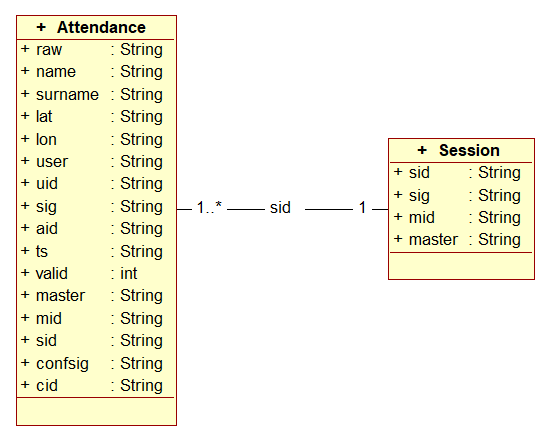
\includegraphics[width=0.6\textwidth]{material/classmodel}
    \caption{Dijagram klasa SPIM i SESS objekata}
\end{figure}
\begin{description}[align=right,labelwidth=2cm,noitemsep]
    \item [raw] serijalizirana string JSON verzija objekta
    \item [name] ime studenta
    \item [surname] prezime studenta
    \item [lat] geografska širina student
    \item [lon] geografska dužina student
    \item [user] ZAMGER korisničko ime studenta
    \item [uid] User ID - SHA2 hex hash javnog ključa studenta
    \item [sig] hex potpis SPIM-a (user:lat:lot:ts)
    \item [aid] Attendance ID - hex SHA2 hash \texttt{sig} potpisa
    \item [ts] vrijeme na studentovom uređaju
    \item [valid] validation cache
    \item [master] ZAMGER korisničko ime profesora
    \item [mid] Master ID - SHA2 hex hash javnog ključa profesora
    \item [sid] Session ID - identifikator profesorove sesije
    \item [confsig] Master Conf. profesorov hex potpis (sid:aid)
    \item [cid] Confirmation ID - SHA2 hex hash confsig-a
\end{description}

\paragraph*{}
Fizički predstavljen opisani SPIM objekat manji je od 1 KB te je pored brzog NFC isl. elektronskog transfera moguće izvršiti prenos alternativnim metodama, kao posebno pogodna čini se QR kod reprezentacija\cite{soon2008qr} i prenos, koja može biti vrlo korisna u slučaju da nijedan od uređaja ne posjeduje NFC modem. Navedeni modus nije implementiran u aplikaciji i dat je kao sugestija zaobilaženja hardverskih ograničenja, primjer QR oblika ranije datog SPIM objekta prikazan je na slici \ref{img:qr}.

\paragraph*{}
Dati QR prikaz je čitljiv ali je vidno uočljiva gustina zapisa koja može predstavljati problem u slučaju lošije kvalitete medija prikaza, u tom slučaju, kompletan SPIM paket moguće je značajno smanjiti zamjenom korištenog RSA kriptosistema za kriptosistem baziran na eliptičnim krivim, budući da su ključevi korišteni u tom slučajnu znatno kraći\cite{atmelecc}, dužina navedenog potpisa bila bi smanjena sa 512 na minimalno 71 bajt\cite{cheneau2009ecc} navedeni pristup nije prihvaćen u okviru ovog rada zbog povećanja kompleksnosti pokaznog sistema, no praktična implementacija moguća je bez većih programskih izmjena.

\begin{figure}[H]
    \centering
    \begin{subfigure}{.5\textwidth}
        \centering
        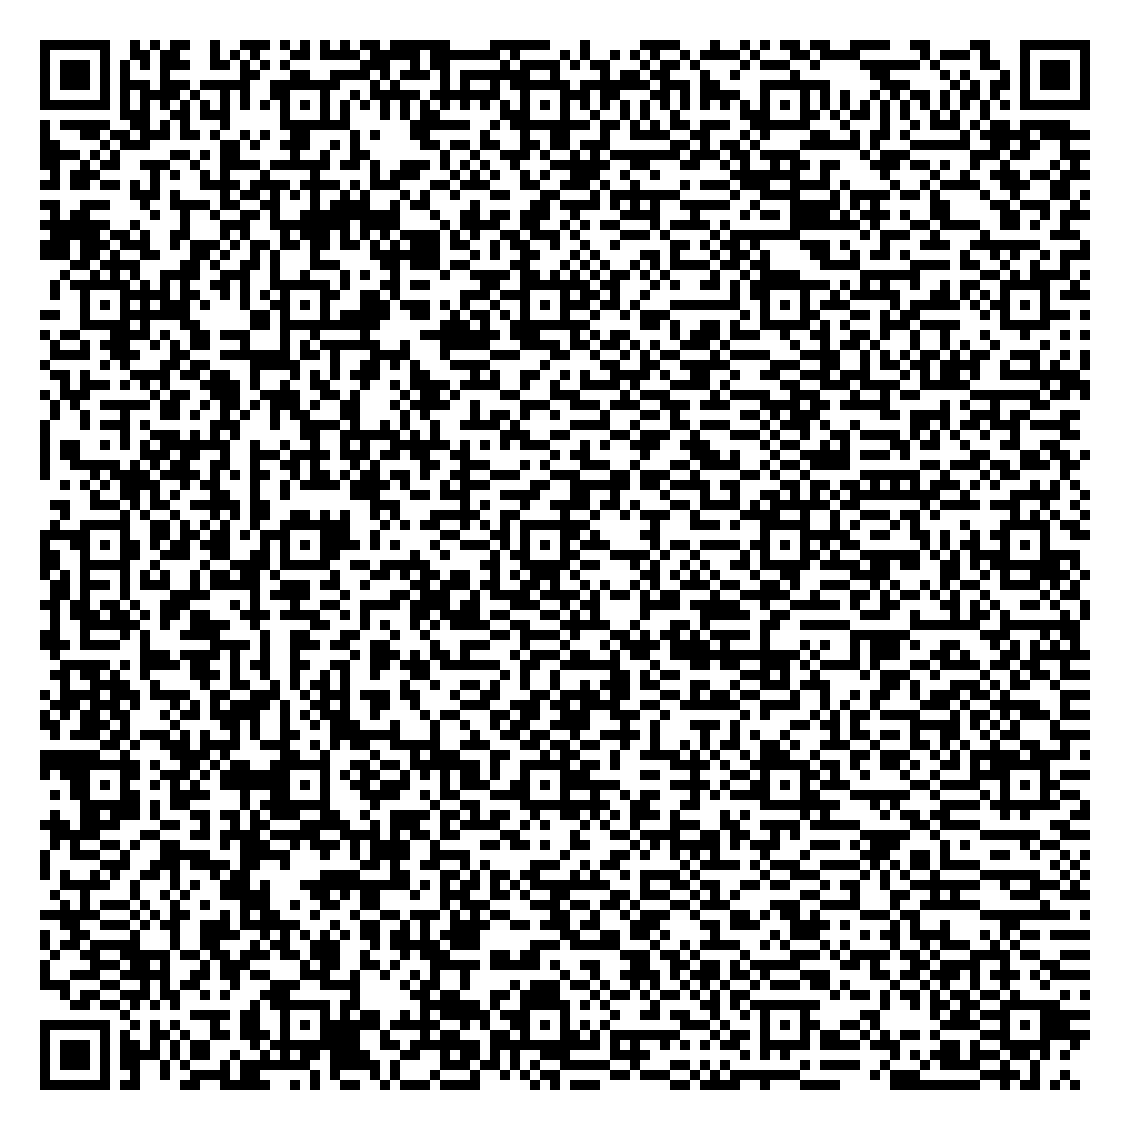
\includegraphics[width=.8\textwidth]{material/logit_qr}
        \caption{oblik korištenjem RSA potpisa}
        \label{img:qr_rsa}
    \end{subfigure}%
    \begin{subfigure}{.5\textwidth}
        \centering
        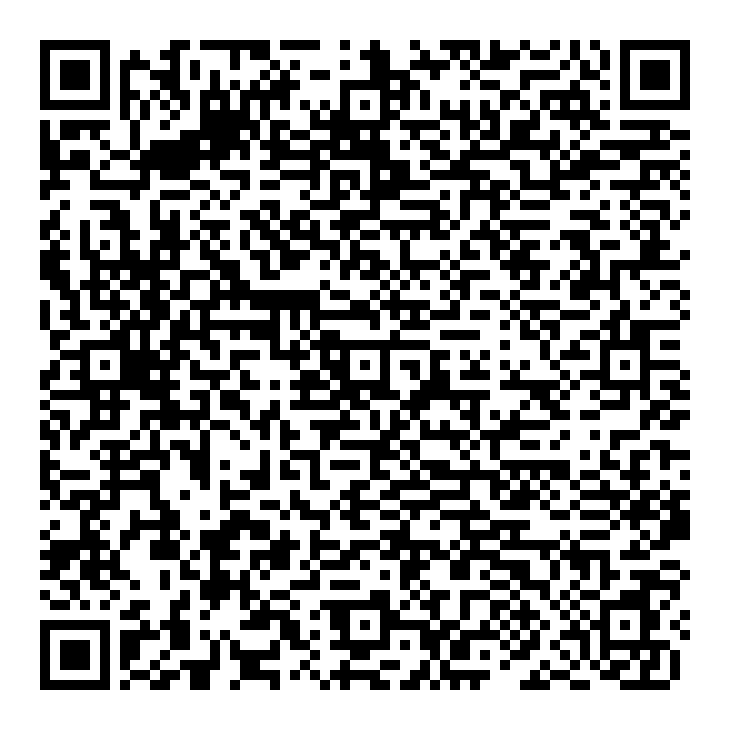
\includegraphics[width=.8\textwidth]{material/logit_qr_ec}
        \caption{oblik korištenjem ECC potpisa}
        \label{img:qr_ecc}
    \end{subfigure}
    \caption{QR oblik SPIM objekta}%
    \label{img:qr}
\end{figure}

\subsection{SESS paket}
Dodatno se za SESS objekat prilikom finaliziranja sesije na LAPI serveru vrši prikupljanje svih CID potpisa koji pripadaju datoj sesiji, te se CID vrijednosti ulančane hronološkim redoslijedom potpisuju LAPI ključem koji se nalazi samo na LAPI hardverskom uređaju, stoga je sigurnost LAPI servera od ključne važnosti za sigurnost ukupnog sistema. Ovako potvrđena sesija ne može biti naknadno mijenjana, lažirana ili porečena izvan LAPI izvršnog okruženja.

\cleardoublepage
\section{Pregled implementacije}
\subsection{MainActivity}
Nakon prvobitnog pokretanja aplikacije a za daljnje uspješno korištenje neophodno je izvršiti autentifikaciju korisnika putem nekog već postoječeg korisničkog repozitorija, te generisati pripadajući virtualizirani sigurni element. Navedene aktivnosti izvršavaju se unutar \texttt{MainActivity} glavnog početnog prozora Logit aplikacije, prikaz relevantnog dijela koda za generisanje virtualiziranog sigurnog elementa dat je u listingu ispod.

\begin{minted}{python}
    KeyPairGenerator kpg = KeyPairGenerator.getInstance(
            "RSA", "AndroidKeyStore");
    Calendar start = Calendar.getInstance();
    Calendar end = Calendar.getInstance();
    end.add(Calendar.YEAR, 1);

    KeyPairGeneratorSpec spec =
            new KeyPairGeneratorSpec.Builder(this).setAlias("etf_logit_" + ts)
                    .setKeySize(2048)
                    .setSubject(new X500Principal("CN=users.etf.ba"))
                    .setSerialNumber(BigInteger.valueOf(tsLong))
                    .setStartDate(start.getTime()).setEndDate(end.getTime()).build();

    kpg.initialize(spec);

    KeyPair kp = kpg.generateKeyPair();

    KeyStore ks = KeyStore.getInstance("AndroidKeyStore");
    ks.load(null);
\end{minted}

\paragraph*{}
Sigurnosni element generisan kao u primjeru iznad dalje se pohranjuje na korisničkom uređaju, gdje privatni dio nikada ne napušta uređaj i dostupan je isključivo Logit aplikaciji putem Android KeyStore providera. Javni dio se koristi kao dio identifikatora korisnika, te se dodatno pohranjuje i na Logit API korisnički repozitorij za potrebe identifikacije i verifikacije potpisa lokacijskog paketa.

\subsection{LogitAPDUService}
Ekstenzija Androidovog native interfejsa \texttt{HostApduService} koji za instaliranu aplikaciju sa \texttt{android.permission.BIND\_NFC\_SERVICE} permisijom vrši pokretanje HCE emulatora prilikom svakog starta operativnog sistema, emulator se u ovom slučaju ponaša kao generički NFC NTAG sa korisnički programiranom memorijom u obliku NDEF poruke koja prenosi jedinstveni potpisan studentski lokacijski dokaz. Navedena servisna komponenta aplikacije aktivna je svaki put dok je i ekran uređaja aktivan ili dok korisnik sam ne zaustavi pripadajući servis. Navedene funkcionalnosti postižu se uključivanjem dijela koda datog u nastavku unutar \texttt{<application>} direktive manifest fajla.

\begin{minted}{python}
    <service
        android:name=".LogitApduService"
        android:permission="android.permission.BIND_NFC_SERVICE">
        <intent-filter>
            <action android:name="android.nfc.cardemulation.action.HOST_APDU_SERVICE" />

            <category android:name="android.intent.category.DEFAULT" />
        </intent-filter>

        <meta-data
            android:name="android.nfc.cardemulation.host_apdu_service"
            android:resource="@xml/apduservice" />
    </service>
\end{minted}

\paragraph*{}
Nadalje \texttt{LogitAPDUService} sadrži logiku za ispravno konstruisanje i formatiranje NDEF paketa\cite{tindef} lokacijskog dokaza i njegovo potpisivanje, te ostalu neophodnu kriptografsku obradu. U nastavku će biti dat prikaz kompletnog servisa sa komentarima relevantnih dijelova.

\begin{minted}{python}
    final static int APDU_INS = 1;
    final static int APDU_P1 = 2;
    final static int APDU_P2 = 3;
    final static int APDU_SELECT_LC = 4;
    final static int APDU_READ_LE = 4;
    final static int FILEID_CC = 0xe103;
    final static int FILEID_NDEF = 0xe104;
    final static byte INS_SELECT = (byte) 0xa4;
    final static byte INS_READ = (byte) 0xb0;
    final static byte INS_UPDATE = (byte) 0xd6;
    final static byte P1_SELECT_BY_NAME = (byte) 0x04;
    final static byte P1_SELECT_BY_ID = (byte) 0x00;
    final static int DATA_OFFSET = 5;

    final static byte[] DATA_SELECT_NDEF = {(byte) 0xd2, (byte) 0x76, (byte) 0x00, (byte) 0x00, (byte) 0x85, (byte) 0x01, (byte) 0x01};
    final static byte[] RET_COMPLETE = {(byte) 0x90, (byte) 0x00};
    final static byte[] RET_NONDEF = {(byte) 0x6a, (byte) 0x82};
    final static byte[] FILE_CC = {
            (byte) 0x00, (byte) 0x0f,       // CCLEN - CC container size
            (byte) 0x20,                    // Mapping version
            (byte) 0x04, (byte) 0xff,       // MLe - max. read size
            (byte) 0x08, (byte) 0xff,       // MLc - max. update size

            // TLV Block (NDEF File Control)
            (byte) 0x04,                    // Tag - Block type
            (byte) 0x06,                    // Length
            (byte) 0xe1, (byte) 0x04,       // File identifier
            (byte) 0x04, (byte) 0xff,       // Max. NDEF file size
            (byte) 0x00,                    // R permission
            (byte) 0x00,                    // W permission
    };
\end{minted}

\paragraph*{}
Deklariše konstantne vrijednosti brojnih dijelova neophodnih za kontrukciju standardne NDEF poruke, između ostalog capability fajl koji predstavlja svojevrsno zaglavlje NDEF paketa.

\paragraph*{}
Metoda generateSignature instancira lokacijske servise i vrši konstukciju paketa lokacijskog dokaza kao i kriptografskih primitiva neophodnih za potpisivanje istog. Za konstrukciju lokacijskog dokaza neophodno je pribaviti trenutno vrijeme uređaja, to je prikazano u narednom dijelu koda.

\begin{minted}{python}
    Long tsLong = System.currentTimeMillis() / 1000;
    String ts = tsLong.toString();
    byte[] signature;
\end{minted}

\paragraph*{}
Nakon toga vršti se instanciranje i učitavanja Android KeyStore objekta koji sadrži korisnički par ključeva neophodnih za potpisivanje lokacijskog paketa.

\begin{minted}{python}
    KeyStore ks = KeyStore.getInstance("AndroidKeyStore");
    ks.load(null);
    KeyStore.ProtectionParameter pp = new KeyStore.PasswordProtection(null);
\end{minted}

\paragraph*{}
Nadalje iz \texttt{KeyStore} objekta učitava se najažurniji virtualizirani sigurnosni element.

\begin{minted}{python}
    Enumeration<String> aliases = ks.aliases();
    String alias = aliases.nextElement();
    Entry entry = ks.getEntry(alias, pp);
\end{minted}

\paragraph*{}
Zbog potrebe za što kompaktnijim prenosom podataka za sve vrijednosti gdje je to moguće generišu se hash preslikavanja koja se kasnije koriste za verifikaciju i pohranjivanje. Za potrebe generisanja hash vrijednosti instancirase SHA-256 \texttt{MessageDigest} objekat.

\begin{minted}{python}
    MessageDigest md = MessageDigest.getInstance("SHA-256");
\end{minted}

\paragraph*{}
Iz virtualiziranog sigurnog elementa dalje učitavamo korisnički certifikat sa javnim ključem, te za potrebe verifikacije identiteta heksadecimalnu reprezentaciju njegove hash vrijednosti pripremamo za uključenje u paket lokacijskog dokaza.

\begin{minted}{python}
    Certificate c = ks.getCertificate(alias);
    byte [] pubKey = c.getPublicKey().getEncoded();
    md.update(pubKey, 0, pubKey.length);
    byte [] pubKeyHash = md.digest();
    String pubKeyHashString = LogitApplication.toHext(pubKeyHash);
\end{minted}

\paragraph*{}
Zatim iz virtualiziranog sigurnog elementa korištenjem korisničkog privatnog ključa pripremamo objekat koji vrši potpisivanje lokacijskog paketa.

\begin{minted}{python}
    Signature s = Signature.getInstance("SHA256withRSA");
    s.initSign(((PrivateKeyEntry) entry).getPrivateKey());
    SharedPreferences userData = getSharedPreferences("UserData", 0);
\end{minted}

\paragraph*{}
Dio lokacijskog paketa koji je pokriven korisničkim digitalnim potpisom sadrži korisničko ime, lokacijske parametre geografske dužine i širine, te vrijeme uređaja u trenutku kreiranja digitalnog potpisa.

\begin{minted}{python}
    String sigPkg = userData.getString("user", "unknown") +
            ":" + location.getLatitude() +
            ":" + location.getLongitude() +
            ":" + ts;
\end{minted}

\paragraph*{}
Takav paket se potpisuje i bilježi se njegova SHA-256 preslikana vrijednost za potrebe verifikacije.

\begin{minted}{python}
    s.update(sigPkg.getBytes("UTF-8"));
    signature = s.sign();
\end{minted}

\paragraph*{}
Osnovni potpisani lokacijski paket se proširuje vrijednostima generisanih SHA-256 preslikavanja i osnovnim korisničkim podacima, te se prosljeđuje metodi createMessage koja formira standardizovan NDEF paket, takav spreman NDEF paket stavlja se na raspolaganje komponenti za prenos putem NFC protokola.

\begin{minted}{python}
    msg = "{\"lat\":\"" + location.getLatitude() +
            "\", \"lon\":\"" + location.getLongitude() +
            "\", \"ts\":\"" + ts +
            "\", \"sig\":\"" + LogitApplication.toHext(signature) +
            "\", \"uid\":\"" + pubKeyHashString +
            "\", \"name\":\"" + LogitApplication.toHext(userData.getString("name", "unknown").getBytes("UTF-8")) +
            "\", \"surname\":\"" + LogitApplication.toHext(userData.getString("surname", "unknown").getBytes("UTF-8")) +
            "\", \"user\":\"" + userData.getString("user", "unknown") + "\"}";

    NdefMessage ndef = createMessage(msg.getBytes("UTF-8"));
    byte[] ndefarray = ndef.toByteArray();

    mNdefFile = new byte[ndefarray.length + 2];

    mNdefFile[0] = (byte) ((ndefarray.length & 0xff00) >> 8);
    mNdefFile[1] = (byte) (ndefarray.length & 0x00ff);

    System.arraycopy(ndefarray, 0, mNdefFile, 2, ndefarray.length);

    logitApp.setMessage(mNdefFile);
\end{minted}

\subsection{processCommandApdu}
Budući da se u prikazanom slučaju vrši emulacija pasivnog NTAG uređaja, APDU servis se izvršava u slave modu i zaprima instukcije od strane master uređaja, neophodno je implementirati parser petlju i logiku za komunikaciju sa master uređajem, unutar koje se vrši prepoznavanje zadatih instrukcija i priprema adekvatan odgovor, navedena logika implementirana je unutar \texttt{processCommandApdu} metode. Kompletna logika emulacije tag uređaja svodi se na prosljeđivanje adekvatnog zaglavlja taga i READ FROM TO binarnog protokola za čitanje memorije koju šalje master, stoga glavninu navedene metode čini jedna switch petlja koja u skladu sa zadatom komandom vraća zaglavlje ili raspon bita emuliranog taga, u ovom slučaju sadržaj koji se emulira je prošireni lokacijski paket iznad. Detalje opisane metode možete pogledati u prilogu koda u dodatku.

\subsection{AttendanceActivity}
Za ostvarivanje pune funkcionalnosti aplikacije neophodna je bila implementacija master moda za prikupljanje i obradu NDEF paketa, u ovom slučaju korisničkih potpisa, enkapsuliranih u obliku potpisanog lokacijskog paketa. \texttt{AttendanceActivity} vrši navedenu funkcionalnost te dodatno vrši provjeru valjanosti potpisa i podataka korisničkih lokacijskih paketa. Verifikacija korisničkih lokacijskih paketa vrši se tako što se korisnički slave podaci o vremenu i lokaciji porede sa podacima o vremenu i lokaciji master uređaja, time se osigurava zaštita od napada lažiranja podataka, te bi za takvu vrstu prevare bila neophodna koluzija dva aktera suprostavljenih interesa, što znatno umanjuje vjerovatnoću takvih napada. Moguće je podesiti vrijednosti dozvoljenih odstupanja verifikacijskih parametara izmjenom koda za tu namjenu datog u nastavku.

\begin{minted}{python}
    final long timediff = System.currentTimeMillis() / 1000 - Long.parseLong(tmpAttn.getTs());
    final Location userLocation = new Location("MOCK");
    userLocation.setLatitude(Double.valueOf(tmpAttn.getLat()));
    userLocation.setLongitude(Double.valueOf(tmpAttn.getLon()));
    if (Build.VERSION.SDK_INT >= 23
            && ContextCompat.checkSelfPermission(that, android.Manifest.permission.ACCESS_FINE_LOCATION ) == PackageManager.PERMISSION_GRANTED
            && ContextCompat.checkSelfPermission(that, android.Manifest.permission.ACCESS_COARSE_LOCATION) == PackageManager.PERMISSION_GRANTED
            || Build.VERSION.SDK_INT < 23) {
        FusedLocationProviderClient mFusedLocatiionClient = LocationServices.getFusedLocationProviderClient(that);
        mFusedLocatiionClient.getLastLocation().addOnSuccessListener(new OnSuccessListener<Location>() {
            @Override
            public void onSuccess(Location location) {
                Float locdiff = userLocation.distanceTo(location);
                if (Math.abs(timediff) < 300) {
                    if (locdiff < 100) {
                        // Lokacija i vrijeme SLAVE uređaja su VALIDNI
                    } else {
                        Toast.makeText(that, "Greška: lokacije udaljene " + locdiff.intValue() + " metara.", Toast.LENGTH_LONG).show();
                    }
                } else {
                    Toast.makeText(that, "Greška: vrijeme nije tačno ili je TAG zastario.", Toast.LENGTH_LONG).show();
                }
\end{minted}

\paragraph*{}
Da bi se izbjegla obaveza reimplementiranja NDEF protokola za podatke primljene putem NFC podatkovnog interfejsa Android nudi predefinisani intent filter za direktnu manipulaciju NDEF poruka, te je za njegovo korištenje potrebno dodati ispod prikazani kod unutar manifest fajla Android aplikacije. Korištenjem ovog filtera programer kao rezultat uspješnog NFC prenosa dobija standardizovanu NDEF poruku spremnu za obradu. Ovaj interfejs se koristi unutar \texttt{AttendanceActivity}.

\begin{minted}{python}
<intent-filter>
    <action android:name="android.nfc.action.NDEF_DISCOVERED" />

    <category android:name="android.intent.category.DEFAULT" />

    <data android:mimeType="application/octet-stream" />
</intent-filter>
\end{minted}

\paragraph*{}
Ostatak koda unutar \texttt{AttendanceActivity} klase koristi se za prikaz i obradu elemenata korisničkog interfejsa master moda za prikupljanje korisničkih potpisa.
	\chapter{Funkcionalni opis Logit rješenja} \label{ch:man}
\begin{enumerate}
    \item \textbf{Uspostavite internet konekciju} prema uputama vašeg nastavnika.
    \begin{enumerate}
        \item potrebno je da na mreži bude dostupna Logit serverska aplikacija i certifikacijski repozitorij za uspješnu prijavu i korištenje, dostupnost možete provjeriti posjetom na \url{https://logit.mine.nu:5000}
    \end{enumerate}
    \item \textbf{Uključite lokacijske usluge} vašeg Android mobilnog uređaja.
    \begin{enumerate}
        \item detaljno uputstvo možete pronaći na \url{https://support.google.com/accounts/answer/3467281?hl=hr}
    \end{enumerate}
    \item \textbf{Omogućite NFC komunikaciju} na vašem Android mobilnom uređaju i \textbf{isključite Android Beam} uslugu za optimalan rad aplikacije.
    \begin{enumerate}
        \item \texttt{Settings > NFC > Enable}
        \item \texttt{Settings > NFC > Android Beam > Disable}
        \item više detalja za navedene postavke pročitajte na \url{https://support.google.com/nexus/answer/2781895?hl=hr}
    \end{enumerate}
    \item Ukoliko niste, \textbf{omogućite sigurnosnu funkcionalnost zaključavanja vašeg ekrana}
    \begin{enumerate}
        \item Android OS nudi usluge integrisane sigurnosti mobilnih uređaja, te je Keystore funkcionalnost sigurnog pohranjivanja privatnih ključeva usko vezana za ostale sigurnostne postavke, stoga omogućite zaključavanje ekrana slijedeći uputstvo na \url{https://support.google.com/nexus/answer/2819522?hl=hr}
    \end{enumerate}
    \item Prihvatite poziv za alpha testiranje posjetom na \url{https://play.google.com/apps/testing/ba.unsa.etf.logit} i nastavite na Play Store te \textbf{instalirajte aplikaciju}
    \begin{enumerate}
        \item ukoliko vaš mobilni uređaj nije izlistan kao podržan obratite se vašem nastavniku i biti će vam izdat jedinstveni NFC Certifikat, koji ćete koristiti za bilježenje prisustva
    \end{enumerate}
    \item \textbf{Pokrenite Logit aplikaciju}
    \item \textbf{Unesite vaše ZAMGER korisničke podatke}, ovi podatci koriste se jednokratno za provjeru valjanosti identiteta prije generisanja vašeg para ključeva, vaša lozinka ne ostaje pohranjena na Logit sistem i prenosi se https kanalom prema ZAMGER servisu
    \item Aplikacija je spremna za korištenje i ne mora biti pokrenuta u prednjem planu za prijavu prisustva, \textbf{za optimalne rezultate} dovoljno je da upalite ekran vašeg Android uređaja na “lock screen” i prislonite na Android uređaj nastavnika.
    \item \textbf{Ukoliko želite koristiti aplikaciju u nastavničkom modu} i prikupljati prisustvo, dovoljno je da pokrenete Logit aplikaciju u prednjem planu te prislonite vaš uređaju studentskom uređaju u skladu sa korakom 8.
\end{enumerate}

%\pagebreak[4]
\section{Nastavnički način rada}
\paragraph*{}
Pokretanjem glavnog prozora Logit aplikacije ulazite u mod za prikupljanje studentskih potpisa prisustva. Ovaj zaslon podijeljen je na četiri komponente, opisi kako slijedi u nastavku.

\begin{figure}[H]
    \centering
    
\includegraphics[width=0.6\textwidth]{material/manual/01-head}
    \caption{Zaglavlje aplikacije prikazuje aktivnog korisnika}
\end{figure}

\begin{figure}[H]
    \centering
    
\includegraphics[width=0.6\textwidth]{material/manual/02-menu}
    \caption{Glavni izbornik, opisi funkcionalnosti u nastavku}
\end{figure}

\begin{description}[noitemsep,align=right,labelwidth=2cm]
    \item [Dugme 1] služi za ručno osvježavanje trenutne lokacije
    \item [Dugme 2] koristite za provjeru valjanosti ključeva korištenih pri potpisu
    \item [Dugme 3] sinhronizacija trenutne sesije na Logit server, svi potpisi se pohranjuju u jednu sesijsku cjelinu i brišu sa mobilnog uređaja (kreira se nova sesija)
    \item [Dugme 4] otvara e-mail klijent po izboru korisnika u cilju lakše prijave grešaka
\end{description}

\begin{figure}[H]
    \centering
    
\includegraphics[width=0.6\textwidth]{material/manual/03-geobar}
    \caption{Trenutno zabilježena lokacija korisničkog uređaja}
\end{figure}

\begin{figure}[H]
    \centering
    
\includegraphics[width=0.6\textwidth]{material/manual/04-attns}
    \caption{Ordinalno numerisan spisak prisutnih studenata}
\end{figure}
	\chapter{Sigurnosna analiza} \label{chapter:sec}
Sa aspekta teorije igara\cite{davis2012game} u okruženju dva igrača unutar kooperativne igre\cite{nash1953two} pronalazak optimalne strategije je uvijek prost u slučaju da međusobna saradnja maksimizira profit oba igrača, stoga ukoliko se prikupljanje obostrano korisnih dokaza u vidu prisustva predavanju svede u navedene okvire tada se radi o kolaborativnoj igri studenta i predavača te ne bi trebao da se javlja problem međusobnog povjerenja, dovoljan uvjet za sigurnost takvog sistema je ispravna tehnička implementacija kriptografskih rješenja koja sprječavaju napade jednostranim falsifikovanjem dokaza. Aplikacija izrađena u okviru ovog rada zadovoljava preduvjete kolaborativne igre \textbf{dva igrača}, budući da je prisustvo studenata dokaz prisustva profesora i obratno, njihov odnos je kriptografski osiguran strukturom nalik na hijerarhiju uređenog hash skupa, takva struktura osigurava osobine neizmjenjivosti i neporecivosti.

\paragraph*{}
Sa tehničkog aspekta jedan vektor napada predstavlja lažiranje lokacije ili vremena na korisničkim uređajima, stim što je preduvjet za uspješnost takvog napada koluzija predavača i studenta da priskrbe korist na štetu treće strane, tj. institucije korisnice sistema i neučesnika u koluziji. Moguće je otežati izvodivost i osigurati detekciju ovog napada programskim mjerama zabrane i bilježenja korištenja ručno podešene (\textit{en. mock}) lokacije uređaja i provjerom vremenskih podataka potpisa na LAPI strani koja osigurava pouzdane vremenske podatke. Dodatno treba napomenuti da cijena opisanog napada raste proporcionalno broju studenata učesnika jer svi studenti koji žele priskrbiti neostvarenu korist moraju učestvovati u koluziji, također svi neučesnici imaju štetu (npr. predavanje nije održano u predviđenom terminu zbog odsustva predavača, naknadno falsifikovan dokaz o održavanju u koluziji sa dva studenta, svi ostali studenti gube bodove za prisustvo), stoga i direktu korist od razotkrivanja napada.

\paragraph*{}
Sigurnost izloženog rješenja polazi i počiva na pretpostavci povjerljivosti i jedinstvenosti \textbf{korisničkog privatnog ključa} koji nikada ne napušta okruženje emuliranog sigurnosnog elementa korisničkog Android uređaja, ukoliko se naruši data pretpostavka ne postoje garancije sigurnosti sistema. Postoji jedan-na-jedan asocijacija između korisnika i sigurnosnog uređaja, gdje se zbog prirode problema i niskog nivoa prijetnje kao dovoljan uvjet asocijacije uzima posjedovanje uređaja, no takav uvjet ne može se smatrati dovoljnim za čvrst dokaz identiteta te se za namjene gdje je to neophodno preporučuje implementacija dodatnog faktora biometrijske identifikacije unutar pouzdanog okruženja (ne na korisničkom uređaju).
	\chapter{Zaključak}
Aplikacija izrađena u okviru ovog rada zadovoljava zahtjeve navedene u postavci zadatka i pripadajućem opisu. Korištene su savremene kriptografske metode za implementaciju sigurnosno osjetljivih funkcionalnosti i osigurano je stabilno okruženje za neometano funkcionisanje aplikacije, dodatno je prema zahtjevima uspješno realiziran NFC komunikacijski interfejs između studentskih i instruktorskih mobilnih uređaja. U cilju lakšeg skaliranja težilo se je što više koristiti standardizovane tehnologije, posebno kada je u pitanju NFC, gdje je dodatno implementirana emulacija NTAG vrste taga kao NDEF medija, time je omogućeno da se sistem u budućnosti prilagodi stacionarnim NFC čitačima i korištenju samostalnih NFC tagova.

\paragraph*{}
Pokušana je pilot primjena sistema u saradnji sa nastavnim osobljem na predmetu "Tehnologije sigurnosti" u školskoj godini 2017/18. kojom prilikom je sačinjen spisak studenata i izvršene pripreme sistema. Navedena pilot primjena okončana je neuspješno zbog otvorenih sigurnosnih pitanja u integraciji sa postojećim sistemima, nedostatka resursa i nepostojanja pokusnog sistema pogodnog za projekte u ranoj fazi testiranja, stoga u cilju povećanja inovativnosti i razvoja novih usluga preporučuje se izrada pokusnih \textit{(en. staging)} sistema odvojenih od produkcijskog u okviru Elektrotehničkog fakulteta u Sarajevu.

\paragraph*{}
Tokom pripreme pilot primjene identifikovano je da značajan broj studenata ne posjeduje NFC omogućene mobilne uređaje, te su za njihove potrebe izrađene NTAG216 NFC token naljepnice, no primjena navedenih tokena uvjetovana je dodatnim istraživanjem i doradom Logit sistema za rad sa NTAG216 da bi osigurao isti ili viši nivo sigurnosnih garancija od onog koje pruža Android izvršno okruženje. Kao dodatna smjernica u istraživanju dat je prijedlog korištenja QR kodova za namjenu supstitucije u slučajevima nepostojanja tehničkih predispozicija za upotrebu sistema na strani korisnika, navedena tehnologija može dati dobre rezultate u praktičnoj primjeni i zavređuje dalji istraživački tretman.

\paragraph*{}
Krajnja težnja Logit rješenja je obuhvatanje cjelokupnog sistema autentifikacije i modeliranje relacija povjerenja u materijalnopravnom okruženju, kroz izradu proširive bazne platforme koja može obuhvatiti digitalizaciju mnoštva svakodnevnih administrativnih zadataka jedne institucije, sa tim ciljem daljnje istraživačke napore zavređuje usmjeriti ka razvoju stabilne PKI infrastrukture, kao i digitalizaciji vjerodostojnih institucionalnih registara poput registra ispita sa ciljem digitalizacije studentskog indeksa i srodnih dokumenata.
%	\begin{appendices}
%		\chapter{Izvorni kod}
\section{LAPI izvorni kod}
{\small Repo: \url{https://github.com/koljenovic/logit-node/}}
\begin{minted}{text}
.
├── Logit
│   ├── Logit
│   │   ├── __init__.py
│   │   ├── logit.db
│   │   └── static
│   └── logit.wsgi
├── README.md
└── README.md~
\end{minted}
\subsection{\small \url{__init__.py}}
\inputminted{python}{../logit-node/Logit/Logit/__init__.py}

\section{Android izvorni kod}
{\small Repo: \url{https://github.com/koljenovic/logit/tree/master/android/app/src/main}}
\begin{minted}{text}
.
├── AndroidManifest.xml
├── ic_launcher-web.png
├── java
│   └── ba
│       └── unsa
│           └── etf
│               └── logit
│                   ├── api
│                   │   └── LogitService.java
│                   ├── AttendanceActivity.java
│                   ├── AttendanceAdapter.java
│                   ├── LogitApduService.java
│                   ├── LogitApplication.java
│                   ├── MainActivity.java
│                   └── model
│                       ├── Attendance.java
│                       ├── Place.java
│                       ├── Session.java
│                       └── User.java
└── res
    ├── ---
    │ 
\end{minted}

\pagebreak[4]
\subsection{\small \url{AndroidManifest.xml}}
\inputminted{xml}{../logit/android/app/src/main/AndroidManifest.xml}

\subsection{\small \url{model/Attendance.java}}
\inputminted{java}{../logit/android/app/src/main/java/ba/unsa/etf/logit/model/Attendance.java}

\subsection{\small \url{model/Place.java}}
\inputminted{java}{../logit/android/app/src/main/java/ba/unsa/etf/logit/model/Place.java}

\subsection{\small \url{model/Session.java}}
\inputminted{java}{../logit/android/app/src/main/java/ba/unsa/etf/logit/model/Session.java}

\subsection{\small \url{model/User.java}}
\inputminted{java}{../logit/android/app/src/main/java/ba/unsa/etf/logit/model/User.java}

\subsection{\small \url{api/LogitService.java}}
\inputminted{java}{../logit/android/app/src/main/java/ba/unsa/etf/logit/api/LogitService.java}

\subsection{\small \url{AttendanceActivity.java}}
\inputminted{java}{../logit/android/app/src/main/java/ba/unsa/etf/logit/AttendanceActivity.java}

\subsection{\small \url{AttendanceAdapter.java}}
\inputminted{java}{../logit/android/app/src/main/java/ba/unsa/etf/logit/AttendanceAdapter.java}

\subsection{\small \url{LogitApduService.java}}
\inputminted{java}{../logit/android/app/src/main/java/ba/unsa/etf/logit/LogitApduService.java}

\subsection{\small \url{LogitApplication.java}}
\inputminted{java}{../logit/android/app/src/main/java/ba/unsa/etf/logit/LogitApplication.java}

\subsection{\small \url{MainActivity.java}}
\inputminted{java}{../logit/android/app/src/main/java/ba/unsa/etf/logit/MainActivity.java}
%	\end{appendices}
	\backmatter
	\bibliographystyle{IEEEtranETF}
	\bibliography{main}
\end{document}